\documentclass[11pt]{article}
\usepackage[margin=1in]{geometry}
\usepackage{amsmath,amssymb,amsthm,mathtools,bm}
\usepackage{booktabs,array,tabularx}
\usepackage{graphicx}
\usepackage{tikz}
\usetikzlibrary{arrows.meta,decorations.markings,calc,positioning}
\usepackage[dvipsnames]{xcolor}
\usepackage{tcolorbox}
\usepackage{enumitem}
\usepackage{dsfont}
\usepackage[numbers,sort&compress]{natbib}
\usepackage[colorlinks=true,linkcolor=RoyalBlue,citecolor=ForestGreen,urlcolor=RoyalBlue]{hyperref}
\usepackage[capitalise]{cleveref}

% ---------- macros (same as keldysh_mori_zwanzig_v2.tex, plus a few) ----------
\newcommand{\Tr}{\operatorname{Tr}}
\newcommand{\Lc}{\mathcal{L}}
\newcommand{\Pc}{\mathcal{P}}
\newcommand{\Qc}{\mathcal{Q}}
\newcommand{\Kc}{\mathcal{K}}
\newcommand{\Gc}{\mathcal{G}}
\newcommand{\Dc}{\mathcal{D}}
\newcommand{\ee}{\mathrm{e}}
\newcommand{\dd}{\mathrm{d}}
\newcommand{\cl}{\mathrm{c}}
\newcommand{\qu}{\mathrm{q}}
\newcommand{\rhoS}{\rho_{S}}
\newcommand{\rhoB}{\rho_{B}}
\newcommand{\ket}[1]{|#1\rangle}
\newcommand{\bra}[1]{\langle#1|}
\newcommand{\kket}[1]{|#1\rangle\!\rangle}
\newcommand{\bbra}[1]{\langle\!\langle#1|}
\newcommand{\avg}[1]{\langle#1\rangle}
\newcommand{\acomm}[2]{\{#1,#2\}}
\newcommand{\comm}[2]{[#1,#2]}
\newcommand{\sx}{\sigma_x}
\newcommand{\sy}{\sigma_y}
\newcommand{\sz}{\sigma_z}
\newcommand{\Id}{\mathds{1}}
\renewcommand{\Re}{\operatorname{Re}}
\renewcommand{\Im}{\operatorname{Im}}
\DeclareMathOperator{\sgn}{sgn}

\newtcolorbox{keybox}[1][]{colback=RoyalBlue!4,colframe=RoyalBlue!60,
  fonttitle=\bfseries,title={#1},boxrule=0.6pt,arc=2pt,left=4pt,right=4pt,top=3pt,bottom=3pt,breakable}
\newtcolorbox{exbox}[1][]{colback=ForestGreen!4,colframe=ForestGreen!60,
  fonttitle=\bfseries,title={#1},boxrule=0.6pt,arc=2pt,left=4pt,right=4pt,top=3pt,bottom=3pt,breakable}
\newtcolorbox{warnbox}{colback=Orange!6,colframe=Orange!70,boxrule=0.6pt,arc=2pt,
  left=4pt,right=4pt,top=3pt,bottom=3pt,breakable}
\tcbuselibrary{breakable}

\theoremstyle{definition}
\newtheorem{exercise}{Exercise}[section]
\newtheorem{definition}{Definition}[section]
\theoremstyle{plain}
\newtheorem{proposition}{Proposition}[section]
\newtheorem{lemma}[proposition]{Lemma}
\newtheorem{theorem}[proposition]{Theorem}
\theoremstyle{remark}
\newtheorem*{remark}{Remark}

\title{\textbf{A Qubit in a Bosonic Bath}\\[4pt]
\large Keldysh, Nakajima--Zwanzig and Mori:\\ ten lectures on one open quantum system\\[6pt]
\normalsize Self-contained lecture notes with worked examples, numerics and exercises}
\author{Notes prepared with Claude for J.~O.~Sofo}
\date{19 October 2026}

\begin{document}
\maketitle

\begin{abstract}
\noindent These notes develop, from scratch and in one consistent notation, the three
standard languages for the dynamics of a small quantum system coupled to a large
environment: the Keldysh (closed-time-path) formalism, the Nakajima--Zwanzig and
time-convolutionless projection-operator master equations, and Mori's projection onto
operators. The thread that ties them together is a single model, a two-level system
(qubit) coupled linearly to a bath of harmonic oscillators through a general coupling
operator $S=\cos\theta\,\sz+\sin\theta\,\sx$, which interpolates between pure dephasing
($\theta=0$) and the dissipative two-level system of Leggett \emph{et al.} Every formal
construction is followed immediately by its evaluation for this model, and a committed
Python script produces the figures, so that each approximation can be compared with an
exact reference. The last lecture turns the machinery toward quantum sensing. References
to the original literature are given throughout.
\end{abstract}

\begin{warnbox}
\small\textbf{How to use these notes.} Each lecture is meant for one sitting of two to three
hours with pen and paper. Boxes labelled \emph{Example} carry the running model; boxes
labelled \emph{Key point} are the statements you should be able to reproduce from memory.
Exercises at the end of each lecture have solutions or detailed hints in
\cref{sec:solutions}. The numerical figures are generated by
\texttt{figures/spin\_boson\_numerics.py}; running it takes about a minute and every
parameter is listed in \cref{sec:numerics}. These notes are self-contained but build on the
shorter working note \texttt{keldysh\_mori\_zwanzig\_v2} in the same folder, whose notation
they share.\\[3pt]
\textbf{About the references.} Entries carried over from \texttt{refs.bib} were checked
against publisher records on 30~September~2026. Entries added for these notes are marked
in the \texttt{.bib} file; their bibliographic data were written from memory of the
literature and should be verified before being quoted in a publication. All equations were
derived independently and the central ones are checked numerically in \cref{sec:numerics}.
\end{warnbox}

\tableofcontents
\clearpage

%=====================================================================
\section*{Lecture 0: The map of the course}
\addcontentsline{toc}{section}{Lecture 0: The map of the course}
\label{sec:overview}

\paragraph{The problem.}
A small quantum system $S$ (here: a qubit) is coupled to a large environment $B$ (here: a bath of harmonic oscillators).
The full dynamics is unitary, but we only ever look at the system, so what we want is the \emph{reduced} dynamics: either the reduced density matrix $\rhoS(t)=\Tr_B\rho(t)$, or the expectation values and correlation functions of system operators.
Three formalisms were invented, by different communities and for different purposes, to do exactly this:
\begin{itemize}[itemsep=1pt]
\item \textbf{Keldysh} (Schwinger~\cite{Schwinger1961}, Keldysh~\cite{Keldysh1964}): write expectation values as a path integral or a diagrammatic series on a closed time contour that runs forward with $U$ and backward with $U^\dagger$.
  Natural for many-body systems, Green's functions and field theory.
\item \textbf{Nakajima--Zwanzig} (Nakajima~\cite{Nakajima1958}, Zwanzig~\cite{Zwanzig1960}) and its time-convolutionless (TCL) variant~\cite{Shibata1977,Chaturvedi1979}: project the full density matrix onto the ``relevant'' part $\rhoS\otimes\rhoB$ and derive a closed, exact integro-differential equation for $\rhoS(t)$.
  Natural for small systems and for questions about positivity, memory and master equations.
\item \textbf{Mori} (Mori~\cite{Mori1965}, Zwanzig~\cite[Ch.~8]{ZwanzigBook}): project \emph{operators} (Heisenberg picture) onto a chosen set of slow variables and derive a generalized Langevin equation.
  Natural for hydrodynamics, response functions and continued-fraction approximations.
\end{itemize}

\paragraph{The thesis.}
The three formalisms are not three theories; they are three bookkeeping schemes for the same perturbation series.
The precise statements, proved in the course, are:
\begin{keybox}[The three bridges]
\begin{enumerate}[itemsep=1pt]
\item Ordering superoperators along the real time axis \emph{is} Keldysh contour ordering (\cref{sec:lec3}).
  The ``classical/quantum'' Keldysh rotation is the pair of superoperators $A^\cl=\tfrac12\{A,\cdot\}$, $A^\qu=[A,\cdot]$.
\item The Nakajima--Zwanzig (NZ) memory kernel is the sum of \emph{irreducible} real-time diagrams of the reduced propagator, and the NZ equation is its Dyson equation (\cref{sec:lec5}).
  TCL is the same Dyson equation solved for a time-local generator (\cref{sec:lec6}).
\item Mori's memory function is the \emph{retarded self-energy} of the projected operator; for the full operator basis with the Heisenberg-adjoint inner product it is the adjoint of the NZ kernel (\cref{sec:lec8}).
\end{enumerate}
In all three, a Gaussian bath enters only through two kernels: the symmetrized noise $S(t)$ (Keldysh component $D^K$) and the response $\chi(t)$ (retarded component $D^R$).
\end{keybox}

\paragraph{The running example.}
Everything is worked out for
\begin{equation}
  H=\frac{\omega_0}{2}\sz+\sum_k\omega_kb_k^\dagger b_k
  +\big(\cos\theta\,\sz+\sin\theta\,\sx\big)\otimes\sum_kg_k\big(b_k+b_k^\dagger\big),
  \label{eq:model-intro}
\end{equation}
the spin-boson model with a general linear coupling.
The mixing angle $\theta$ lets us switch between the two textbook limits without changing the formalism: $\theta=0$ is pure dephasing (exactly solvable, the sensor's workhorse) and $\theta=\pi/2$ is transverse coupling (relaxation, the damped qubit).
Intermediate $\theta$ is unitarily equivalent to the biased dissipative two-level system of Leggett \emph{et al.}~\cite{Leggett1987}, as we show in \cref{sec:lec2}.
A Lorentzian spectral density makes the model numerically exact through the pseudomode mapping~\cite{Garraway1997,Tamascelli2018}, so each approximation in the course can be compared with the truth (\cref{sec:numerics}).

\paragraph{The route.}
\Cref{sec:lec1,sec:lec2} set up the language (Liouville space; the model and its bath).
\Cref{sec:lec3,sec:lec4} derive the Keldysh structure and the diagram rules from the von Neumann equation.
\Cref{sec:lec5,sec:lec6} derive NZ and TCL and identify them with the Dyson equation.
\Cref{sec:lec7} goes to the path integral: Feynman--Vernon, the polaron frame and the noninteracting-blip approximation.
\Cref{sec:lec8} does Mori and connects it to the other two.
\Cref{sec:lec9} rewrites the qubit problem as a Keldysh field theory, so the reader can recognize the structures in the many-body literature.
\Cref{sec:lec10} turns the machinery to quantum sensing: which protocol measures which bath kernel, and why non-Markovian memory changes precision scaling.

\paragraph{Prerequisites.}
Quantum mechanics at the level of second quantization for bosons, the interaction picture and the Dyson series; a first exposure to density matrices.
No prior knowledge of Keldysh, projection operators or path integrals is assumed.
Units: $\hbar=k_B=1$.

\clearpage

%=====================================================================
\section{Lecture 1: Liouville space, superoperators and the qubit}
\label{sec:lec1}

Open-system theory is linear algebra on the space of operators. This lecture makes that
space concrete for a qubit, so that in later lectures every abstract superoperator can be
written as a $4\times4$ matrix and checked by hand.

\subsection{Operators as vectors}

Let $\mathcal H$ be a $d$-dimensional Hilbert space. The linear operators on $\mathcal H$
form a $d^2$-dimensional vector space, \emph{Liouville space}, with the
Hilbert--Schmidt inner product
\begin{equation}
  (A,B)\equiv\Tr\big(A^\dagger B\big).
  \label{eq:HS}
\end{equation}
We write $\kket{A}$ for an operator regarded as a vector and $\bbra{A}B\rangle\!\rangle=(A,B)$.
For a qubit ($d=2$) an orthonormal basis is
\begin{equation}
  \kket{e_0}=\tfrac{1}{\sqrt2}\Id,\quad \kket{e_1}=\tfrac{1}{\sqrt2}\sx,\quad
  \kket{e_2}=\tfrac{1}{\sqrt2}\sy,\quad \kket{e_3}=\tfrac{1}{\sqrt2}\sz ,
\end{equation}
since $\Tr(\sigma_i\sigma_j)=2\delta_{ij}$. Any operator is $X=\tfrac12(x_0\Id+\bm x\cdot\bm\sigma)$ with
$x_\mu=\Tr(\sigma_\mu X)$, and a density matrix is
\begin{equation}
  \rho=\tfrac12\big(\Id+\bm r\cdot\bm\sigma\big),\qquad \bm r=\avg{\bm\sigma},\qquad |\bm r|\le1 ,
  \label{eq:bloch}
\end{equation}
the Bloch vector~\cite{Bloch1946}. Throughout the notes we use the \emph{coefficient
convention}: a superoperator $\mathcal M$ is represented by the $4\times4$ matrix $M_{\mu\nu}$
defined by $\mathcal M\sigma_\nu=\sum_\mu M_{\mu\nu}\sigma_\mu$, i.e.\
$M_{\mu\nu}=\tfrac12\Tr(\sigma_\mu\,\mathcal M\sigma_\nu)$, which is also the matrix in the
orthonormal basis $\kket{e_\mu}$. It acts on the coefficient vector $(x_0,x_x,x_y,x_z)$.

A second, equivalent representation is \emph{vectorization}: stack the columns of the
$d\times d$ matrix $X$ into a $d^2$-vector $\mathrm{vec}(X)$. The identity
\begin{equation}
  \mathrm{vec}(AXB)=\big(B^{T}\otimes A\big)\,\mathrm{vec}(X)
  \label{eq:vec}
\end{equation}
turns every ``sandwich'' into a matrix. This is what the numerical script uses
(\cref{sec:numerics}); the coefficient convention is what we use on paper. They are
related by the unitary change of basis from $\{\ket i\bra j\}$ to $\{\sigma_\mu/\sqrt2\}$.

\subsection{Superoperators}

A \emph{superoperator} is a linear map on Liouville space. The two elementary ones are
left and right multiplication by a fixed operator $A$,
\begin{equation}
  A^{+}X\equiv AX,\qquad A^{-}X\equiv XA .
  \label{eq:leftright}
\end{equation}
The superscripts anticipate \cref{sec:lec3}: $A^+$ acts on the ket side of $\rho$ (the
forward branch of the Keldysh contour), $A^-$ on the bra side (the backward branch).
Left and right multiplications by different operators always commute,
$A^+B^-=B^-A^+$, because $(AX)B=A(XB)$. In vectorized form,
$A^+=\Id\otimes A$ and $A^-=A^T\otimes\Id$ by \cref{eq:vec}.

\paragraph{Products of operators.}
What is the superoperator of a product $AB$? On the left side the order is preserved,
on the right side it is reversed:
\begin{equation}
  (AB)^{+}X=ABX=A^{+}B^{+}X,\qquad
  (AB)^{-}X=XAB=(XA)B=B^{-}A^{-}X,
\end{equation}
so that
\begin{equation}
  \boxed{\;(AB)^{+}=A^{+}B^{+},\qquad (AB)^{-}=B^{-}A^{-}.\;}
  \label{eq:product-rule}
\end{equation}
The map $A\mapsto A^+$ is an algebra homomorphism, the map $A\mapsto A^-$ is an
\emph{anti}-homomorphism (in vectorized form this is just $(AB)^T=B^TA^T$). This
innocent-looking reversal is the entire origin of the Keldysh contour: a string of
operators acting on the bra side of $\rho$ is applied in the opposite order, which is why
the backward branch is anti-time-ordered (\cref{sec:lec3}). Two consequences follow
immediately: $(A^n)^\pm=(A^\pm)^n$ for powers of a single operator, and the commutators
\begin{equation}
  [A^{+},B^{+}]=\big([A,B]\big)^{+},\qquad [A^{-},B^{-}]=-\big([A,B]\big)^{-},\qquad [A^{+},B^{-}]=0 ,
  \label{eq:super-commutators}
\end{equation}
the minus sign in the second being the anti-homomorphism again. The Hermitian conjugates
with respect to \cref{eq:HS} are $(A^{+})^\dagger=(A^\dagger)^{+}$ and $(A^{-})^\dagger=(A^\dagger)^{-}$,
since $\Tr[Y^\dagger AX]=\Tr[(A^\dagger Y)^\dagger X]$ and $\Tr[Y^\dagger XA]=\Tr[(YA^\dagger)^\dagger X]$.

From these we build the two combinations that organize everything that follows:
\begin{equation}
  \boxed{\;A^{\cl}\equiv\tfrac12\big(A^{+}+A^{-}\big),\quad A^{\cl}X=\tfrac12\{A,X\};\qquad
  A^{\qu}\equiv A^{+}-A^{-},\quad A^{\qu}X=[A,X].\;}
  \label{eq:clqu}
\end{equation}
Inversely $A^\pm=A^\cl\pm\tfrac12A^\qu$. For Hermitian $A$ both $A^\cl$ and $A^\qu$ map Hermitian
operators to Hermitian operators (the anticommutator and $i\times$commutator of Hermitian
operators are Hermitian; note $A^\qu X$ is anti-Hermitian for Hermitian $X$ and the $i$ is
supplied by the Liouvillian).

\begin{keybox}[Three properties used constantly]
For any operator $A$ on $\mathcal H$ and any $X$:
\begin{enumerate}[itemsep=1pt]
\item $\Tr(A^\qu X)=\Tr[A,X]=0$: the quantum superoperator maps into the traceless subspace.
\item $\Tr(A^\cl X)=\Tr(AX)$: the classical superoperator ``measures'' $A$.
\item $[A^\cl,A^\qu]=0$ and $A^\cl A^\qu X=\tfrac12\big(A^2X-XA^2\big)=\tfrac12(A^2)^\qu X$.
\end{enumerate}
The first two are the cyclicity of the trace. The third follows from $A^+A^-=A^-A^+$.
\end{keybox}

\paragraph{Products in the rotated variables.}
The product rule \cref{eq:product-rule} translates into the $\cl/\qu$ language as
\begin{equation}
\begin{aligned}
  (AB)^{\cl}&=\tfrac12\{A^{\cl},B^{\cl}\}+\tfrac18\{A^{\qu},B^{\qu}\}+\tfrac14\big([A^{\cl},B^{\qu}]+[A^{\qu},B^{\cl}]\big),\\
  (AB)^{\qu}&=\tfrac12\{A^{\cl},B^{\qu}\}+\tfrac12\{A^{\qu},B^{\cl}\}+[A^{\cl},B^{\cl}]+\tfrac14[A^{\qu},B^{\qu}],
\end{aligned}
  \label{eq:product-clqu}
\end{equation}
obtained by inserting $A^\pm=A^\cl\pm\tfrac12A^\qu$ into $(AB)^\cl=\tfrac12(A^+B^++B^-A^-)$ and
$(AB)^\qu=A^+B^+-B^-A^-$ (\cref{ex:1-5}). When the superoperators of $A$ and $B$ commute,
which is the case whenever $A$ and $B$ act on different tensor factors (system and bath)
or more generally whenever $[A,B]=0$, the commutator terms drop and the rule collapses to
the familiar Keldysh rule for composite fields,
\begin{equation}
  (AB)^{\cl}=A^{\cl}B^{\cl}+\tfrac14A^{\qu}B^{\qu},\qquad (AB)^{\qu}=A^{\cl}B^{\qu}+A^{\qu}B^{\cl}\qquad([A,B]=0),
  \label{eq:product-clqu-commuting}
\end{equation}
which is exactly how the interaction vertex $\Lc_I=-i(S\otimes B)^\qu$ will acquire its
``one classical, one quantum leg'' structure in \cref{sec:lec3}. For a single operator,
$A=B$, \cref{eq:product-clqu-commuting} gives $(A^2)^\cl=(A^\cl)^2+\tfrac14(A^\qu)^2$ and
$(A^2)^\qu=2A^\cl A^\qu$, which is property~3 of the key box above.

\paragraph{The Liouvillian.}
The von Neumann equation $\dot\rho=-i[H,\rho]$ reads $\dot\rho=\Lc\rho$ with
\begin{equation}
  \Lc=-i\big(H^{+}-H^{-}\big)=-iH^\qu ,\qquad \rho(t)=\ee^{\Lc t}\rho(0)=\ee^{-iHt}\rho(0)\ee^{iHt}.
\end{equation}
Its adjoint with respect to \cref{eq:HS}, defined by $(A,\Lc X)=(\Lc^\dagger A,X)$, is
$\Lc^\dagger A=+i[H,A]$, the Heisenberg-picture generator: $\avg{A}_t=(A,\rho(t))=(\ee^{\Lc^\dagger t}A,\rho(0))$.
This duality, state picture versus operator picture, is exactly the duality between the
Nakajima--Zwanzig projection (\cref{sec:lec5}) and the Mori projection (\cref{sec:lec8}).

\begin{exbox}[Example 1.1: the free qubit in Bloch form]
Take $H_S=\frac{\omega_0}{2}\sz$. Using $[\sz,\sx]=2i\sy$, $[\sz,\sy]=-2i\sx$,
\begin{equation}
  \Lc_S\sx=-i\tfrac{\omega_0}{2}[\sz,\sx]=\omega_0\sy,\qquad
  \Lc_S\sy=-\omega_0\sx,\qquad \Lc_S\Id=\Lc_S\sz=0 .
\end{equation}
In the coefficient convention, with rows and columns ordered $(\Id,\sx,\sy,\sz)$,
\begin{equation}
  \Lc_S=\begin{pmatrix}0&0&0&0\\0&0&-\omega_0&0\\0&\omega_0&0&0\\0&0&0&0\end{pmatrix},
  \qquad
  \ee^{\Lc_St}:\ \begin{cases}x_x\mapsto\cos(\omega_0t)\,x_x-\sin(\omega_0t)\,x_y,\\ x_y\mapsto\sin(\omega_0t)\,x_x+\cos(\omega_0t)\,x_y,\end{cases}
  \label{eq:LS-bloch}
\end{equation}
so $\dot r_x=-\omega_0r_y$, $\dot r_y=\omega_0r_x$: the Bloch vector precesses
counter-clockwise about $\hat z$ at $\omega_0$. The eigenvalues of $\Lc_S$ are
$0,0,\pm i\omega_0$, with eigenvectors $\Id,\sz$ (populations) and
$\sigma_\mp=\tfrac12(\sx\mp i\sy)$ (coherences): $\Lc_S\sigma_-=-i\omega_0\sigma_-$. In the
basis $\{\ket0\bra0,\ket0\bra1,\ket1\bra0,\ket1\bra1\}$ the matrix is
$\operatorname{diag}(0,-i\omega_0,+i\omega_0,0)$, which is the ``vectorized'' form.
\end{exbox}

\begin{exbox}[Example 1.2: $\cl$ and $\qu$ superoperators of the coupling operator]
The running model couples the bath to $S=\cos\theta\,\sz+\sin\theta\,\sx$. We need
$S^\cl$ and $S^\qu$ as $4\times4$ matrices. First the building blocks:
\begin{align}
  \sz^\cl:&\ \Id\mapsto\sz,\ \sz\mapsto\Id,\ \sx\mapsto0,\ \sy\mapsto0; &
  \sz^\qu:&\ \sx\mapsto2i\sy,\ \sy\mapsto-2i\sx,\ \Id\mapsto0,\ \sz\mapsto0;\notag\\
  \sx^\cl:&\ \Id\mapsto\sx,\ \sx\mapsto\Id,\ \sy\mapsto0,\ \sz\mapsto0; &
  \sx^\qu:&\ \sy\mapsto2i\sz,\ \sz\mapsto-2i\sy,\ \Id\mapsto0,\ \sx\mapsto0 .
\end{align}
(The $\cl$ map of a Pauli matrix swaps it with the identity; the $\qu$ map rotates the
other two Pauli matrices into each other with a factor $\pm2i$.) In matrix form, rows and
columns ordered $(\Id,\sx,\sy,\sz)$,
\begin{equation}
  S^\cl=\begin{pmatrix}0&\sin\theta&0&\cos\theta\\ \sin\theta&0&0&0\\ 0&0&0&0\\ \cos\theta&0&0&0\end{pmatrix},\qquad
  S^\qu=2i\begin{pmatrix}0&0&0&0\\ 0&0&-\cos\theta&0\\ 0&\cos\theta&0&-\sin\theta\\ 0&0&\sin\theta&0\end{pmatrix}.
  \label{eq:SclSqu}
\end{equation}
Read off the three properties: the first row of $S^\qu$ vanishes (traceless-valued), the
first row of $S^\cl$ is $(0,\sin\theta,0,\cos\theta)=\tfrac12\Tr(S\sigma_\nu)$ (it measures $S$),
and $S^\qu$ is $2i$ times the generator of rotations about the axis
$\hat n=(\sin\theta,0,\cos\theta)$ on the Bloch vector, which is what $[S,\cdot]$ should be.
Note also $S^\qu$ annihilates $S$ itself (the vector $(0,\sin\theta,0,\cos\theta)$) and the
identity. For $\theta=0$ the matrices reduce to the pure-dephasing case
$\sz^\cl=\text{``swap }\Id\leftrightarrow\sz\text{''}$, $\sz^\qu=2i\,(\sx\!\to\!\sy\!\to\!-\sx)$.
\end{exbox}

\subsection{Dynamical maps}

For a factorized initial state $\rho(0)=\rhoS(0)\otimes\rhoB$, the reduced state at time $t$
is a linear function of the initial reduced state,
\begin{equation}
  \rhoS(t)=\Pi(t)\rhoS(0),\qquad \Pi(t)X\equiv\Tr_B\!\big[\ee^{\Lc t}\big(X\otimes\rhoB\big)\big].
  \label{eq:map}
\end{equation}
$\Pi(t)$ is the \emph{dynamical map}; in Liouville space it is a $d^2\times d^2$ matrix
with $\Pi(0)=1$. Three properties follow directly from \cref{eq:map}:
\emph{trace preservation}, $\Tr_S\Pi(t)X=\Tr X$ (first row of the Bloch matrix is
$(1,0,0,0)$); \emph{Hermiticity preservation}; and \emph{complete positivity}, since
$\Pi(t)$ is a partial trace of a unitary conjugation~\cite[Sec.~8.2.3]{Nielsen2010}.
Complete positivity is equivalent to the existence of a Kraus form
$\Pi X=\sum_kM_kXM_k^\dagger$~\cite{Choi1975}. Maps obtained from \cref{eq:map} with a
\emph{correlated} initial state need not be completely positive, or even
linear in $\rhoS(0)$~\cite{Pechukas1994}; we stay with factorized initial states except
where noted.

What $\Pi(t)$ is \emph{not}, in general, is a semigroup: $\Pi(t+s)\ne\Pi(t)\Pi(s)$. The
bath remembers. The whole subject of these notes is how to write equations of motion for
$\rhoS(t)$ when the map is not a semigroup, and the two standard answers are: a
time-nonlocal (Nakajima--Zwanzig) equation $\dot\rhoS=\Lc_S\rhoS+\int_0^tK(t-s)\rhoS(s)\dd s$, and a
time-local (TCL) equation $\dot\rhoS=\Gc(t)\rhoS(t)$. When $\Gc(t)$ happens to be constant
and of Gorini--Kossakowski--Sudarshan--Lindblad form~\cite{GKS1976,Lindblad1976},
\begin{equation}
  \Gc X=-i[H',X]+\sum_j\gamma_j\Big(L_jXL_j^\dagger-\tfrac12\{L_j^\dagger L_j,X\}\Big),\qquad\gamma_j\ge0,
  \label{eq:GKSL}
\end{equation}
the map is a completely positive semigroup; this is the Markovian limit.

\begin{exbox}[Example 1.3: the pure-dephasing map in Bloch form]
Suppose the only effect of the bath is to multiply the coherence by a real factor:
$\rho_{01}(t)=\rho_{01}(0)\,\ee^{-i\omega_0t-\Gamma(t)}$ with $\Gamma(t)\ge0$ (we will derive this for
$\theta=0$ in \cref{sec:lec4}). Then $r_z$ is constant and $(r_x,r_y)$ rotates and shrinks:
\begin{equation}
  \Pi(t)=\begin{pmatrix}1&0&0&0\\ 0&\ee^{-\Gamma}\cos\omega_0t&-\ee^{-\Gamma}\sin\omega_0t&0\\
  0&\ee^{-\Gamma}\sin\omega_0t&\ee^{-\Gamma}\cos\omega_0t&0\\ 0&0&0&1\end{pmatrix}.
\end{equation}
Its Kraus form has two operators, $M_0=\sqrt{\tfrac{1+\ee^{-\Gamma}}2}\,\ee^{-i\omega_0t\sz/2}$ and
$M_1=\sqrt{\tfrac{1-\ee^{-\Gamma}}2}\,\sz\ee^{-i\omega_0t\sz/2}$, so it is completely positive for
every $\Gamma\ge0$. The TCL generator is $\Gc(t)=\dot\Pi\Pi^{-1}=\Lc_S-\dot\Gamma(t)\,\tfrac14(\sz^\qu)^2$,
where $-\tfrac14(\sz^\qu)^2X=-\tfrac14[\sz,[\sz,X]]=\tfrac12(\sz X\sz-X)$ is the dephasing
dissipator (check with \cref{eq:SclSqu}: $(\sz^\qu)^2\sx=\sz^\qu(2i\sy)=4\sx$, so
$-\tfrac14(\sz^\qu)^2\sx=-\sx$, as it should, while $\Id$ and $\sz$ are annihilated). The generator is of GKSL form with rate $\gamma(t)=\dot\Gamma(t)$, which can be
negative at times when $\Gamma$ decreases: a time-local generator of a completely positive
map need not have positive rates. This is the simplest example of ``non-Markovian but
time-local''.
\end{exbox}

\subsection{Exercises}

\begin{exercise}\label{ex:1-1}
Verify the three properties in the key box above directly from the definitions, and
show that for Hermitian $A$, $(A^\cl)^\dagger=A^\cl$ and $(A^\qu)^\dagger=-A^\qu$ with respect to
the Hilbert--Schmidt product. Conclude that $i A^\qu$ is Hermitian as a superoperator.
\end{exercise}

\begin{exercise}\label{ex:1-2}
Write $\Lc_S$ for $H_S=\frac{\omega_0}{2}\sz$ in the vectorized basis
$\{\ket0\bra0,\ket0\bra1,\ket1\bra0,\ket1\bra1\}$ using \cref{eq:vec}, and find the unitary
$4\times4$ matrix that maps it to \cref{eq:LS-bloch}.
\end{exercise}

\begin{exercise}\label{ex:1-3}
Show that the matrix of $\Pi(t)$ in the coefficient convention has the block form
$\begin{psmallmatrix}1&0\\ \bm c(t)&T(t)\end{psmallmatrix}$ with a $3\times3$ matrix $T$ and a
vector $\bm c$ (the affine Bloch form $\bm r\mapsto T\bm r+\bm c$). Show that positivity
requires $|T\bm r+\bm c|\le1$ for all $|\bm r|\le1$ and that for a unital map ($\bm c=0$) complete
positivity is a stronger condition than this (give the standard counterexample: the
transposition $T=\operatorname{diag}(1,-1,1)$).
\end{exercise}

\begin{exercise}\label{ex:1-4}
Compute $(S^\cl)^2$ and $(S^\qu)^2$ from \cref{eq:SclSqu} and interpret them with property~3
of the key box (use $S^2=\Id$).
\end{exercise}

\begin{exercise}\label{ex:1-5}
Derive \cref{eq:super-commutators} and \cref{eq:product-clqu}, and check the latter on
$A=\sx$, $B=\sy$ (so $AB=i\sz$) using the matrices of Example~1.2 with $\theta=0$ and
$\theta=\pi/2$: verify that $(i\sz)^\cl=i\sz^\cl$ comes out of the right-hand side, including
the commutator terms, which do not vanish here because $[\sx,\sy]\ne0$.
\end{exercise}

\clearpage

%=====================================================================
\section{Lecture 2: The model, its bath, and the two kernels}
\label{sec:lec2}

\subsection{The Hamiltonian and its two faces}

The running model is
\begin{equation}
\begin{aligned}
  H&=H_S+H_B+H_I,\qquad
  H_S=\frac{\omega_0}{2}\sz,\qquad
  H_B=\sum_k\omega_kb_k^\dagger b_k,\\
  H_I&=S\otimes B,\qquad
  S=\cos\theta\,\sz+\sin\theta\,\sx,\qquad
  B=\sum_kg_k\big(b_k+b_k^\dagger\big).
\end{aligned}
  \label{eq:model}
\end{equation}
The qubit has energy splitting $\omega_0$; the bath is a collection of harmonic
oscillators (phonons, photons, the electromagnetic modes of a cavity or a transmission
line, the Gaussian part of a spin bath, etc.); the coupling is linear in the bath
coordinates and couples to a fixed Hermitian qubit operator $S$ with $S^2=\Id$. The angle
$\theta$ is the only new parameter compared with the textbook cases.

\paragraph{Pure dephasing, $\theta=0$.} $H_I=\sz\otimes B$ commutes with $H_S$. Populations
are frozen, coherences decay. This is the model of ``$T_2$'' processes, of the filter-function
formalism in quantum sensing, and of Ramsey and echo experiments~\cite{Ramsey1950,Hahn1950}.
It is exactly solvable for any Gaussian bath (\cref{sec:lec4,sec:lec7}).

\paragraph{Transverse coupling, $\theta=\pi/2$.} $H_I=\sx\otimes B$ flips the qubit. This is
the model of ``$T_1$'' processes: spontaneous and stimulated emission, absorption, and the
associated Lamb shift. In the rotating-wave approximation it becomes the damped
Jaynes--Cummings model, which is again exactly solvable for a single excitation.

\paragraph{The dissipative two-level system.}
For general $\theta$, rotate the qubit about $\hat y$ so that $S$ becomes the new $\sz$:
define $\sz'\equiv S=\cos\theta\sz+\sin\theta\sx$ and $\sx'\equiv\cos\theta\sx-\sin\theta\sz$,
which satisfy the Pauli algebra with $\sy'=\sy$. Then
$\sz=\cos\theta\,\sz'-\sin\theta\,\sx'$ and
\begin{equation}
  H=\frac{\varepsilon}{2}\sz'-\frac{\Delta}{2}\sx'+\sz'\otimes B+H_B,\qquad
  \varepsilon=\omega_0\cos\theta,\quad \Delta=\omega_0\sin\theta .
  \label{eq:leggett-form}
\end{equation}
This is the spin-boson model in the form of Leggett \emph{et al.}~\cite[Sec.~II]{Leggett1987}
and Weiss~\cite[Ch.~3]{Weiss2012}: a particle tunnelling with amplitude $\Delta$ between two
wells with bias $\varepsilon$, whose \emph{position} $\sz'$ is coupled to the bath. Our
$\theta$ is the angle between the energy eigenbasis and the bath's pointer basis. Keep both
pictures in mind: \cref{eq:model} is natural for perturbation theory in the coupling
$g_k$ (the energy eigenstates are a good starting point), while \cref{eq:leggett-form} is
natural for perturbation theory in $\Delta$ after a polaron transformation (the pointer
states are a good starting point). We will use both, in \cref{sec:lec5} and
\cref{sec:lec7} respectively. The two expansions have different domains of validity, and
seeing the same kernel emerge in both is one of the pleasures of the subject.

\begin{warnbox}
\small\textbf{Normalization of the coupling.} Leggett \emph{et al.} write the coupling as
$\tfrac12\sz'\sum_kc_kx_k$ with oscillator coordinates $x_k=(b_k+b_k^\dagger)/\sqrt{2m_k\omega_k}$,
and define $J_{\rm L}(\omega)=\tfrac{\pi}2\sum_kc_k^2/(m_k\omega_k)\,\delta(\omega-\omega_k)$. With
$g_k=c_k/\sqrt{2m_k\omega_k}$ this is $J_{\rm L}(\omega)=\pi\sum_kg_k^2\delta(\omega-\omega_k)$, which coincides with our
$J(\omega)$ of \cref{eq:J} below, \emph{but} their coupling operator is $\sz'/2$ where ours is $\sz'$.
All our bath kernels therefore enter with a factor~4 relative to Leggett's formulas when
the same $J$ is used; equivalently, our $\theta=0$ model with $J$ is Leggett's with $4J$.
We flag this at each place where it matters.
\end{warnbox}

\subsection{Bath correlation function; noise and response}

In the interaction picture with respect to $H_B$, $B(t)=\sum_kg_k(b_k\ee^{-i\omega_kt}+b_k^\dagger\ee^{i\omega_kt})$.
For a thermal bath $\rhoB=\ee^{-\beta H_B}/Z_B$ with $\bar n_k=(\ee^{\beta\omega_k}-1)^{-1}$,
\begin{equation}
  C(t)\equiv\avg{B(t)B(0)}=\sum_kg_k^2\Big[(\bar n_k+1)\ee^{-i\omega_kt}+\bar n_k\ee^{i\omega_kt}\Big]
  =\int_0^\infty\!\frac{\dd\omega}{\pi}\,J(\omega)\Big[\coth\tfrac{\beta\omega}{2}\cos\omega t-i\sin\omega t\Big],
  \label{eq:C}
\end{equation}
where the \emph{spectral density}
\begin{equation}
  J(\omega)\equiv\pi\sum_kg_k^2\,\delta(\omega-\omega_k)\qquad(\omega>0)
  \label{eq:J}
\end{equation}
is the only property of the bath that the system will ever feel (for a Gaussian bath;
see below). $C(t)$ is neither real nor even: $C(-t)=C(t)^*$. Its real and imaginary parts
are the two kernels of the title:
\begin{align}
  S(t)&\equiv\tfrac12\avg{\{B(t),B(0)\}}=\Re C(t)=\int_0^\infty\!\frac{\dd\omega}{\pi}\,J(\omega)\coth\tfrac{\beta\omega}2\,\cos\omega t ,
  \label{eq:S-def}\\
  \chi(t)&\equiv i\,\theta(t)\avg{[B(t),B(0)]}=-2\theta(t)\Im C(t)=2\theta(t)\int_0^\infty\!\frac{\dd\omega}{\pi}\,J(\omega)\sin\omega t ,
  \label{eq:chi-def}
\end{align}
so that $C(t)=S(t)-\tfrac{i}{2}\chi(t)$ for $t>0$. $S$ is the symmetrized
\emph{noise} correlator: it is what a classical measuring device would record as the
fluctuations of $B$. $\chi$ is Kubo's \emph{response} function~\cite{Kubo1957}: if a force
$f(t)$ is applied through $H\to H-f(t)B$, then $\delta\avg{B(t)}=\int\dd s\,\chi(t-s)f(s)$. The
$\theta(t)$ is causality. $S$ depends on temperature through $\coth$; $\chi$ does not depend
on temperature at all for a harmonic bath.

\paragraph{Frequency domain.}
With $f(\omega)=\int_{-\infty}^\infty\dd t\,\ee^{i\omega t}f(t)$,
\begin{equation}
  \chi''(\omega)=\sgn(\omega)\,J(|\omega|),\quad
  S(\omega)=\coth\tfrac{\beta\omega}{2}\;\chi''(\omega),\quad
  C(\omega)=S(\omega)+\chi''(\omega)=2\chi''(\omega)\big[1+n(\omega)\big],
  \label{eq:FDT}
\end{equation}
with $\chi''\equiv\Im\chi$ and $n(\omega)=(\ee^{\beta\omega}-1)^{-1}$ (for $\omega<0$, $1+n(\omega)=-n(|\omega|)$ and $C(\omega)=2J(|\omega|)n(|\omega|)$).
The middle relation is the fluctuation--dissipation theorem~\cite{CallenWelton1951,Kubo1966};
the last one is the statement that $C(\omega)$ at positive frequency is the rate at which the
bath \emph{absorbs} energy $\omega$ (stimulated $1+n$) and at negative frequency the rate at
which it \emph{emits} ($n$), with detailed balance $C(-\omega)=\ee^{-\beta\omega}C(\omega)$. The real
part of the response follows from Kramers--Kronig,
$\chi'(\omega)=\tfrac1\pi\,\mathrm{P}\!\int\dd\omega'\,\chi''(\omega')/(\omega'-\omega)$. These three functions,
$S$, $\chi''$, $C$, are the same information in a thermal bath; out of equilibrium $S$ and
$\chi$ are independent, and keeping them separate is the whole point of the Keldysh
rotation. See~\cite[Sec.~II]{ClerkRMP2010} for a careful discussion of the asymmetric
spectrum $C(\omega)$ and its measurement.

\begin{exbox}[Example 2.1: two spectral densities used throughout]
\emph{Ohmic bath.} $J(\omega)=2\pi\alpha\,\omega\,\ee^{-\omega/\omega_c}$. With Leggett's coupling
normalization (see the warning box) $\alpha$ is the dimensionless Kondo parameter, with the
famous values $\alpha=\tfrac12$ (Toulouse point) and $\alpha=1$ (localization transition at
$T=0$)~\cite[Secs.~IV--V]{Leggett1987}. At $T=0$,
\begin{equation}
  S(t)=2\alpha\,\omega_c^2\,\frac{1-\omega_c^2t^2}{(1+\omega_c^2t^2)^2},\qquad
  \chi(t)=\theta(t)\,\frac{8\alpha\,\omega_c^3\,t}{(1+\omega_c^2t^2)^2},
\end{equation}
both decaying as power laws on the scale $1/\omega_c$. At temperature $T$ and for $t\gg1/\omega_c$,
$S(t)\simeq-2\alpha(\pi T)^2/\sinh^2(\pi Tt)$: the noise correlator becomes negative and
decays exponentially on the thermal time $1/(\pi T)$. The static susceptibility
$\chi(\omega{=}0)=\tfrac2\pi\int_0^\infty\dd\omega\,J(\omega)/\omega=4\alpha\omega_c$ is twice the reorganization energy.

\emph{Lorentzian bath (pseudomode).} $J(\omega)=g^2\,\dfrac{\gamma/2}{(\omega-\Omega)^2+\gamma^2/4}$, a single
broadened mode at $\Omega$ with width $\gamma$. If we allow this $J$ to extend to negative
frequencies (a good approximation when $\Omega\gg\gamma$, and exactly what the pseudomode
construction below assumes), then at $T=0$
\begin{equation}
  C(t)=g^2\,\ee^{-i\Omega t-\gamma|t|/2},\qquad
  S(t)=g^2\,\ee^{-\gamma|t|/2}\cos\Omega t,\qquad
  \chi(t)=2g^2\,\theta(t)\,\ee^{-\gamma t/2}\sin\Omega t ,
  \label{eq:lorentz-kernels}
\end{equation}
and $S(\omega)=J(\omega)+J(-\omega)$, $\chi''(\omega)=J(\omega)-J(-\omega)$, $C(\omega)=2J(\omega)$.
\Cref{fig:bath-kernels} shows these for the parameters used in all numerical figures,
$\Omega=\omega_0$, $\gamma=0.5\,\omega_0$. The limit $\gamma\to\infty$ at fixed $g^2/\gamma$ is a
Markovian (white-noise) bath; the limit $\gamma\to0$ is a single undamped mode.
\end{exbox}

\begin{figure}[t]
\centering
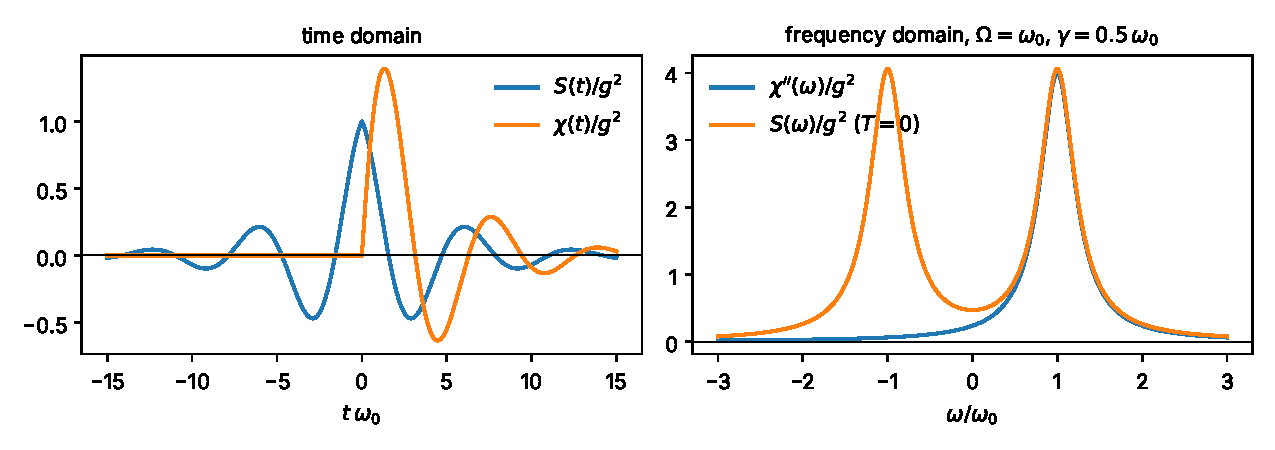
\includegraphics[width=\textwidth]{figures/fig_bath_kernels.pdf}
\caption{The Lorentzian bath used in the numerical examples. Left: noise kernel $S(t)$
(even in $t$) and response kernel $\chi(t)$ (causal, odd before the step function), from
\cref{eq:lorentz-kernels}. Right: $\chi''(\omega)$ and the zero-temperature noise spectrum
$S(\omega)=J(\omega)+J(-\omega)$. A $T_1$ measurement samples these at $\omega=\pm\omega_0$; a
dephasing measurement samples $S$ near $\omega=0$ (\cref{sec:lec10}).}
\label{fig:bath-kernels}
\end{figure}

\subsection{Why only $J(\omega)$ matters: Gaussianity and Wick's theorem}

The bath state is Gaussian (thermal state of a quadratic Hamiltonian) and $B$ is linear
in the $b_k$. Hence all higher moments of $B$ factorize into products of two-point
functions:
\begin{equation}
  \avg{T_{\mathcal C}\,B(z_1)B(z_2)\cdots B(z_{2n})}=\sum_{\text{pairings}}\ \prod_{\text{pairs }(ij)}\avg{T_{\mathcal C}\,B(z_i)B(z_j)},
  \qquad \avg{T_{\mathcal C}\,B(z_1)\cdots B(z_{2n+1})}=0 ,
  \label{eq:wick}
\end{equation}
for any ordering prescription $T_{\mathcal C}$ that is applied consistently inside each pair
(Wick's theorem; see~\cite[Sec.~2.5]{Kamenev2011} for the contour version). Since the
two-point function is built from $J(\omega)$ and $\beta$ alone, so is everything the system
can feel. This is the precise sense in which ``the bath is characterized by its spectral
density''. Non-Gaussian baths (spins, anharmonic modes, fermionic reservoirs with
interactions) need higher cumulants; the formalism of the following lectures survives
with pairings replaced by cumulants~\cite{Schoeller2009}, but we will not need this.

A useful way to say the same thing: for a Gaussian bath, a \emph{linear} coupling, and a
factorized initial state, the reduced dynamics of the system depends on the bath only
through $C(t)$. Any two baths with the same $C(t)$ produce identical $\rhoS(t)$. This is
the basis of the exact reference solution used in the numerics:

\begin{keybox}[The pseudomode mapping (Garraway~\cite{Garraway1997}; Tamascelli \emph{et al.}~\cite{Tamascelli2018})]
Consider the qubit coupled to a \emph{single} oscillator $a$ of frequency $\Omega$, which is
itself damped at rate $\gamma$ by a Markovian environment:
\begin{equation}
  \dot\rho=-i\big[H_S+\Omega a^\dagger a+g\,S\otimes(a+a^\dagger),\rho\big]
  +\gamma\big(a\rho a^\dagger-\tfrac12\{a^\dagger a,\rho\}\big),\qquad \rho(0)=\rhoS(0)\otimes\ket0\bra0 .
  \label{eq:pseudomode}
\end{equation}
The ``bath'' $B_{\rm pm}=g(a+a^\dagger)$ seen by the qubit is Gaussian with
$\avg{B_{\rm pm}(t)B_{\rm pm}(0)}=g^2\ee^{-i\Omega t-\gamma|t|/2}$, which is exactly the Lorentzian
$C(t)$ of \cref{eq:lorentz-kernels}. Therefore the qubit's reduced dynamics in
\cref{eq:pseudomode} is \emph{identical}, to all orders in $g$ and for all times, to its
dynamics in the full Lorentzian bosonic bath. The small Hilbert space (qubit $\otimes$ a
few oscillator levels) makes \cref{eq:pseudomode} trivially solvable numerically. The
price is the negative-frequency tail of $J$; the reward is an exact benchmark for every
approximation in these notes.
\end{keybox}

\subsection{Initial state and pictures}

We take $\rho(0)=\rhoS(0)\otimes\rhoB$ with $\rhoB$ thermal (so $[H_B,\rhoB]=0$ and
$\avg{B}=0$). Physically this means the coupling is switched on at $t=0$, or that the
qubit was prepared by a fast operation that does not disturb the bath. Correlated initial
states (for example the global thermal state of $H$) can be handled, at the price of an
inhomogeneous term in the master equation (\cref{sec:lec5}) or an imaginary-time branch
of the contour (\cref{sec:lec9}).

We will move freely between the Schr\"odinger picture, the interaction picture with
respect to $H_0=H_S+H_B$, and the Heisenberg picture. For the record, in the interaction
picture
\begin{equation}
  \tilde S(t)=\ee^{iH_St}S\ee^{-iH_St}=\cos\theta\,\sz+\sin\theta\big(\sx\cos\omega_0t-\sy\sin\omega_0t\big)
  =\cos\theta\,\sz+\sin\theta\big(\sigma_+\ee^{i\omega_0t}+\sigma_-\ee^{-i\omega_0t}\big),
  \label{eq:S-int}
\end{equation}
with $\sigma_\pm=\tfrac12(\sx\pm i\sy)$. Note that the Heisenberg-picture rotation of $\sx$ is
clockwise, opposite to the Schr\"odinger-picture rotation of the Bloch vector in
\cref{eq:LS-bloch}, as it must be. The $\cos\theta$ part is static, the $\sin\theta$
part oscillates at $\pm\omega_0$: this is why dephasing samples the bath at $\omega\approx0$ and
relaxation samples it at $\omega=\pm\omega_0$.

\subsection{Exercises}

\begin{exercise}\label{ex:2-1}
Derive \cref{eq:C} and check the single-mode case $J(\omega)=\pi g^2\delta(\omega-\omega_b)$ against
$S(t)=g^2(2\bar n+1)\cos\omega_bt$, $\chi(t)=2g^2\theta(t)\sin\omega_bt$. Verify \cref{eq:FDT} for this case.
\end{exercise}

\begin{exercise}\label{ex:2-2}
Prove $\chi''(\omega)=\sgn(\omega)J(|\omega|)$ from \cref{eq:chi-def} and derive the Ohmic kernels
of Example~2.1 at $T=0$. Then show that at finite $T$ and $\omega_c\to\infty$,
$S(t)\to-2\alpha(\pi T)^2/\sinh^2(\pi Tt)$ for $t\ne0$, and explain how a positive-definite
$S(\omega)$ can have a negative $S(t)$ at all $t>0$.
\end{exercise}

\begin{exercise}\label{ex:2-3}
Show that in \cref{eq:pseudomode} the oscillator's two-point function in the absence of
the qubit is $\avg{a(t)a^\dagger(0)}=\ee^{-(i\Omega+\gamma/2)t}$ for $t>0$ (use the quantum
regression theorem, or solve the adjoint equation for $a$), and that the state remains
Gaussian. This is the content of the pseudomode theorem; see~\cite{Tamascelli2018} for
the general statement.
\end{exercise}

\begin{exercise}\label{ex:2-4}
Verify the unitary equivalence \cref{eq:leggett-form}, and show that a bath coupled to
$S=\cos\theta\sz+\sin\theta\sx$ with correlation $C(t)$ is equivalent to \emph{two independent}
baths coupled to $\sz$ and $\sx$ only if the cross-correlation $\cos\theta\sin\theta\,C(t)$ is
dropped. We will see in \cref{sec:lec5} where this cross term goes.
\end{exercise}

\clearpage

%=====================================================================
\section{Lecture 3: The Keldysh contour is already in the von Neumann equation}
\label{sec:lec3}

The Keldysh formalism is usually introduced by declaring a closed time contour and then building Green's functions on it.
In this lecture we go the other way: we expand the reduced density matrix in powers of $H_I$ and watch the contour, the Keldysh rotation and the $2\times2$ matrix structure of the bath propagator appear by themselves.
Nothing is postulated.
At the end we have a set of rules (``contractions'') that \cref{sec:lec4} turns into diagrams.

\begin{figure}[t]
\centering
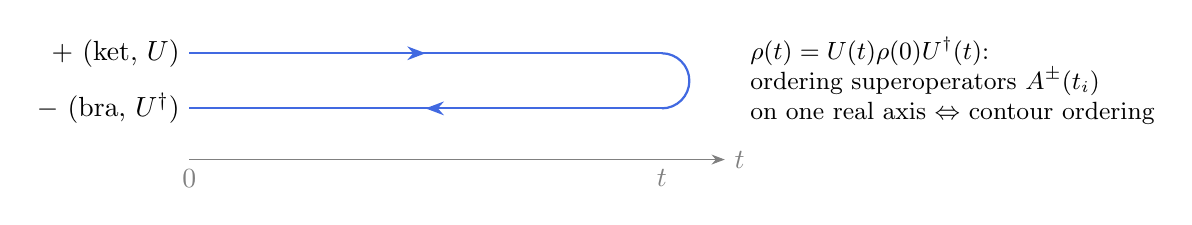
\begin{tikzpicture}[>=Stealth,scale=1.0]
  \draw[thick,RoyalBlue,postaction={decorate},decoration={markings,mark=at position 0.5 with {\arrow{>}}}]
      (0,0.35) -- (6,0.35);
  \draw[thick,RoyalBlue] (6,0.35) arc (90:-90:0.35);
  \draw[thick,RoyalBlue,postaction={decorate},decoration={markings,mark=at position 0.5 with {\arrow{>}}}]
      (6,-0.35) -- (0,-0.35);
  \node[left] at (0,0.35) {$+$ (ket, $U$)};
  \node[left] at (0,-0.35) {$-$ (bra, $U^\dagger$)};
  \draw[->,gray] (0,-1.0) -- (6.8,-1.0) node[right] {$t$};
  \node[below,gray] at (0,-1.0) {$0$};
  \node[below,gray] at (6,-1.0) {$t$};
  \node[right,align=left,font=\small] at (7.0,0.0) {$\rho(t)=U(t)\rho(0)U^\dagger(t)$:\\
  ordering superoperators $A^\pm(t_i)$\\ on one real axis $\Leftrightarrow$ contour ordering};
\end{tikzpicture}
\caption{The Keldysh contour~\cite{Schwinger1961,Keldysh1964}.
The forward branch carries the operators of $U(t)$ acting on the ket side of $\rho(0)$, the backward branch the operators of $U^\dagger(t)$ acting on the bra side.
Contour ordering means: later contour position further from $\rho(0)$.}
\label{fig:contour}
\end{figure}

\subsection{The Dyson series for \texorpdfstring{$\rho$}{rho} and the origin of the contour}
\label{sec:contour-from-vN}

Work in the interaction picture with respect to $H_0=H_S+H_B$, \cref{sec:pictures}: $\tilde\rho(t)=\ee^{iH_0t}\rho(t)\ee^{-iH_0t}$ obeys $\dot{\tilde\rho}=-i[\tilde H_I(t),\tilde\rho]$ with $\tilde H_I(t)=\ee^{iH_0t}H_I\ee^{-iH_0t}$, \cref{eq:int-picture-vN}.
Integrating, $\tilde\rho(t)=\tilde U(t)\rho(0)\tilde U^\dagger(t)$ with
\begin{equation}
  \tilde U(t)=T\exp\Big[-i\!\int_0^t\!\dd s\,\tilde H_I(s)\Big]
  =1-i\!\int_0^t\!\dd t_1\tilde H_I(t_1)-\!\int_0^t\!\dd t_1\!\int_0^{t_1}\!\dd t_2\,\tilde H_I(t_1)\tilde H_I(t_2)+\dots
\end{equation}
Its adjoint is \emph{anti}-time-ordered: in $\tilde U^\dagger$ the later operator stands to the right, $\tilde U^\dagger=1+i\int\tilde H_I-\int_{t_1>t_2}\tilde H_I(t_2)\tilde H_I(t_1)+\dots$

\begin{exbox}[Example 3.1: the second-order term, written out]
Collecting all terms of order $H_I^2$ in $\tilde U\rho(0)\tilde U^\dagger$,
\begin{align}
  \tilde\rho^{(2)}(t)=&-\int_0^t\!\dd t_1\!\int_0^{t_1}\!\dd t_2\,\tilde H_I(t_1)\tilde H_I(t_2)\,\rho(0)
   &&\text{(both on the ket side; time-ordered)}\notag\\
  &-\int_0^t\!\dd t_1\!\int_0^{t_1}\!\dd t_2\,\rho(0)\,\tilde H_I(t_2)\tilde H_I(t_1)
   &&\text{(both on the bra side; anti-time-ordered)}\notag\\
  &+\int_0^t\!\dd t_1\!\int_0^{t}\!\dd t_2\,\tilde H_I(t_1)\,\rho(0)\,\tilde H_I(t_2)
   &&\text{(one on each side; \emph{no} mutual ordering)}.
  \label{eq:rho2}
\end{align}
The third term is the one that looks unusual: $t_1$ and $t_2$ are integrated independently over $[0,t]$, so there is no time ordering between a ket-side and a bra-side operator.
All three terms become a \emph{single} ordering rule once we say that every point on the forward ($+$) branch is ``earlier'' than every point on the backward ($-$) branch, that time runs forward on $+$ and backward on $-$, and that operators are ordered with later contour positions further from $\rho(0)$.
That rule is contour ordering, \cref{fig:contour}.
\end{exbox}

The superoperator language of \cref{sec:lec1} makes the rule automatic.
With $A^{+}X=AX$ and $A^{-}X=XA$,
\begin{equation}
  \tilde\rho^{(2)}(t)=\int_0^t\!\dd t_1\!\int_0^{t_1}\!\dd t_2\,
  \tilde\Lc_I(t_1)\tilde\Lc_I(t_2)\,\rho(0),\qquad
  \tilde\Lc_I(s)=-i\big[\tilde H_I^{+}(s)-\tilde H_I^{-}(s)\big],
  \label{eq:rho2super}
\end{equation}
and multiplying out the two brackets reproduces the three terms of \cref{eq:rho2}: $H^+H^+$ gives the first, $H^-H^-$ gives the second (note $H^-(t_1)H^-(t_2)\rho=\rho H(t_2)H(t_1)$, automatically anti-ordered), and the cross terms $H^+(t_1)H^-(t_2)+H^-(t_1)H^+(t_2)$ give $H(t_1)\rho H(t_2)+H(t_2)\rho H(t_1)$ restricted to $t_1>t_2$, which is the third term with its two orderings separated.
To all orders,
\begin{equation}
  \tilde\rho(t)=T\exp\Big[\int_0^t\!\dd s\,\tilde\Lc_I(s)\Big]\rho(0)
  =\sum_n\int_{t>t_1>\dots>t_n>0}\tilde\Lc_I(t_1)\cdots\tilde\Lc_I(t_n)\,\rho(0),
  \label{eq:dyson-super}
\end{equation}
which is just the Dyson series for the superoperator equation $\dot{\tilde\rho}=\tilde\Lc_I(t)\tilde\rho$ of \cref{eq:int-picture-super}, with $\tilde\Lc_I(t)=\ee^{-\Lc_0t}\Lc_I\ee^{\Lc_0t}$; that this agrees with the operator definition $\tilde\Lc_I=-i[\tilde H_I^+-\tilde H_I^-]$ used in \cref{eq:rho2super} is Lemma~\ref{lem:int-picture}(ii).

\begin{keybox}[Key point 3.1]
Ordinary time ordering of the superoperators $\tilde\Lc_I(t_i)$ along the single real axis $[0,t]$, with a sum over the branch index $\pm$ at each vertex, \emph{is} Keldysh contour ordering.
One never has to think about the contour again: it is encoded in the sign of $\Lc_I$ and the left/right action of $H^\pm$.
Conversely, every Keldysh expression for a one-time expectation value can be read as a Liouville-space string.
\end{keybox}

\subsection{The Keldysh rotation in Liouville space}
\label{sec:rotation-liouville}

The $\pm$ basis is natural for deriving the contour but awkward for calculations, because the two branches are strongly correlated (the trace at the final time glues them together).
The rotation \cref{eq:clqu} separates ``what the two branches have in common'' ($\cl$) from ``how they differ'' ($\qu$).
Since $S$ and $B$ act on different tensor factors, $(SB)^\pm=S^\pm B^\pm$ and $S^\pm$ commutes with $B^\pm$.
Then with $A^\pm=A^\cl\pm\tfrac12A^\qu$,
\begin{align}
  S^{+}B^{+}-S^{-}B^{-}
  &=\big(S^\cl+\tfrac12S^\qu\big)\big(B^\cl+\tfrac12B^\qu\big)
   -\big(S^\cl-\tfrac12S^\qu\big)\big(B^\cl-\tfrac12B^\qu\big)
  =S^\cl B^\qu+S^\qu B^\cl ,
\end{align}
the $S^\cl B^\cl$ and $\frac14S^\qu B^\qu$ terms cancelling.
Hence
\begin{equation}
  \boxed{\;\Lc_I=-i\big(S^{\qu}B^{\cl}+S^{\cl}B^{\qu}\big).\;}
  \label{eq:LIcq}
\end{equation}
The structure ``one $\cl$, one $\qu$ per vertex'' is the same as in the Keldysh action, where the interaction term $H_+-H_-$ is odd in the quantum field and so always contains at least one $\qu$ leg~\cite[Sec.~2.7]{Kamenev2011}.

\paragraph{The two trace identities.}
For an arbitrary operator $Y$ on $\mathcal H_S\otimes\mathcal H_B$ and a bath operator $B$,
\begin{equation}
  \Tr_B\!\big(B^\qu Y\big)=\Tr_B\!\big(BY-YB\big)=0,\qquad
  \Tr_B\!\big(B^\cl Y\big)=\tfrac12\Tr_B\!\big(BY+YB\big)=\Tr_B\!\big(BY\big),
  \label{eq:trace-identities}
\end{equation}
both by cyclicity of the partial trace over the bath factor.
The first identity is the superoperator form of the Keldysh statement that a correlation function whose \emph{latest} point is on a quantum leg vanishes; it is what makes $\avg{\phi_\qu\phi_\qu}=0$ and $\avg{\phi_\cl\phi_\qu}$ retarded~\cite[Sec.~2.6]{Kamenev2011}.
The same identities hold with $S$ in place of $B$ and $\Tr_S$ in place of $\Tr_B$, and they will be used on both sides.

\begin{exbox}[Example 3.2: what $\cl$ and $\qu$ do to a qubit state]
From \cref{eq:SclSqu}, acting on $\rho=\tfrac12(\Id+\bm r\cdot\bm\sigma)$:
\begin{equation}
  S^\cl\rho=\tfrac12\big[(\hat n\cdot\bm r)\Id+\hat n\cdot\bm\sigma\big],\qquad
  S^\qu\rho=i\,(\hat n\times\bm r)\cdot\bm\sigma,\qquad \hat n=(\sin\theta,0,\cos\theta).
\end{equation}
$S^\cl$ produces a traceful object whose weight is the expectation value $\avg{S}=\hat n\cdot\bm r$; $S^\qu$ produces a traceless object proportional to the torque $\hat n\times\bm r$ that a field along $\hat n$ would exert.
A state with $\bm r\parallel\hat n$ (a pointer state of the coupling) has $S^\qu\rho=0$: it does not ``differ between the branches''.
For $\theta=0$ this is the statement that a diagonal density matrix has no quantum component with respect to $\sz$.
This is the operator version of ``the classical field is the physical configuration, the quantum field measures the difference between the two branches''.
\end{exbox}

\subsection{Bath contractions and the \texorpdfstring{$2\times2$}{2x2} Keldysh structure}
\label{sec:contractions}

The basic object is the time-ordered two-point function of bath superoperators,
\begin{equation}
  D^{ab}(t,s)\equiv\Tr_B\!\big[T_{\!\Lc}\,\tilde B^{a}(t)\tilde B^{b}(s)\,\rhoB\big],\qquad a,b\in\{+,-\}\ \text{or}\ \{\cl,\qu\},
\end{equation}
where $T_{\!\Lc}$ puts the later superoperator on the left (closer to the trace).
In the $\pm$ basis the four components are, by direct evaluation for $t>s$,
\begin{center}
\renewcommand{\arraystretch}{1.3}
\begin{tabular}{@{}llll@{}}
\toprule
component & string ($t>s$) & value & Keldysh name \\
\midrule
$D^{++}(t,s)$ & $\Tr_B[B(t)B(s)\rhoB]$ & $C(t-s)$ & time-ordered $D^T$\\
$D^{--}(t,s)$ & $\Tr_B[\rhoB B(s)B(t)]$ & $C(s-t)$ & anti-time-ordered $D^{\tilde T}$\\
$D^{+-}(t,s)$ & $\Tr_B[B(t)\rhoB B(s)]$ & $C(s-t)$ & lesser $D^{<}$\\
$D^{-+}(t,s)$ & $\Tr_B[B(s)\rhoB B(t)]$ & $C(t-s)$ & greater $D^{>}$\\
\bottomrule
\end{tabular}
\end{center}
(For $t<s$ the roles of ``later'' and ``earlier'' are exchanged in the string; the $+-$ and $-+$ entries then keep their form while $++$ and $--$ switch to $C(s-t)$ and $C(t-s)$ respectively.)
These are the four contour-ordered Green's functions of Keldysh theory up to the overall $-i$ of the usual definition, and the familiar linear relation $D^T+D^{\tilde T}=D^<+D^>$ holds entry by entry, which is why the $\pm$ basis is redundant.
Now rotate, using $B^\cl=\frac12(B^++B^-)$ and $B^\qu=B^+-B^-$ on both legs:
\begin{align}
  D^{\cl\cl}(t,s)&=\tfrac14\big(D^{++}+D^{+-}+D^{-+}+D^{--}\big)
   =\tfrac12\big[C(t-s)+C(s-t)\big]=S(t-s),\\
  D^{\cl\qu}(t,s)&=\tfrac12\big(D^{++}-D^{+-}+D^{-+}-D^{--}\big)
   =\theta(t-s)\avg{[B(t),B(s)]}=-i\chi(t-s),\\
  D^{\qu\cl}(t,s)&=\tfrac12\big(D^{++}+D^{+-}-D^{-+}-D^{--}\big)
   =-\theta(s-t)\avg{[B(t),B(s)]}=-i\chi(s-t),\\
  D^{\qu\qu}(t,s)&=D^{++}-D^{+-}-D^{-+}+D^{--}=0 .
\end{align}
(For the middle two lines evaluate separately for $t>s$ and $t<s$ using the table; the $\theta$ functions appear because the ``later'' entry of the table switches.)
In matrix form,
\begin{equation}
  \boxed{\;
  D(t,s)=\begin{pmatrix} D^{\cl\cl} & D^{\cl\qu}\\ D^{\qu\cl} & D^{\qu\qu}\end{pmatrix}
   =\begin{pmatrix} S(t-s) & -i\chi(t-s)\\ -i\chi(s-t) & 0\end{pmatrix}
   \;\leftrightarrow\;
   \begin{pmatrix} D^K & D^R\\ D^A & 0\end{pmatrix},\;}
  \label{eq:LO}
\end{equation}
the Larkin--Ovchinnikov structure~\cite{LarkinOvchinnikov1975,RammerSmith1986}. The zero
in the $\qu\qu$ slot and the retardation of the $\cl\qu$ slot are both consequences of the
first trace identity in \cref{eq:trace-identities}: whenever the \emph{later} superoperator
in the string is $B^\qu$, the trace kills the term. Restricting to $t>s$ and reading off the
entries gives the three contraction rules used from now on:
\begin{equation}
  \Tr_B[\tilde B^{\cl}(t)\tilde B^{\cl}(s)\rhoB]=S(t-s),\qquad
  \Tr_B[\tilde B^{\cl}(t)\tilde B^{\qu}(s)\rhoB]=-i\chi(t-s),\qquad
  \Tr_B[\tilde B^{\qu}(t)\,\cdot\,]=0 .
  \label{eq:contractions}
\end{equation}

\begin{exbox}[Example 3.3: the single-mode bath, and the Lorentzian]
For one mode, $C(t)=g^2[(\bar n+1)\ee^{-i\omega_bt}+\bar n\,\ee^{i\omega_bt}]$, the table gives
$D^{\cl\cl}=g^2(2\bar n+1)\cos\omega_b(t-s)$ and $D^{\cl\qu}=-2ig^2\theta(t-s)\sin\omega_b(t-s)$: the noise
line carries the occupation, the response line does not. In frequency space
$\chi''(\omega)=\pi g^2[\delta(\omega-\omega_b)-\delta(\omega+\omega_b)]$ and $S(\omega)=\coth(\beta\omega/2)\chi''(\omega)$, the FDT checked
by hand. For the Lorentzian bath, \cref{eq:lorentz-kernels} gives the same with
$\omega_b\to\Omega$, $\bar n\to0$ and an extra damping $\ee^{-\gamma|t-s|/2}$ on both lines. In
either case the Keldysh matrix \cref{eq:LO} is, in frequency space,
\begin{equation}
  D(\omega)=\begin{pmatrix} \coth\tfrac{\beta\omega}2\,\chi''(\omega) & -i\chi(\omega)\\ -i\chi(\omega)^* & 0\end{pmatrix},
\end{equation}
which is Kamenev's $D^K=\coth(\beta\omega/2)(D^R-D^A)$ with $D^R=-i\chi$~\cite[Sec.~2.6]{Kamenev2011}.
\end{exbox}

\paragraph{Wick's theorem for superoperators.}
Because the Liouville string $\Tr_B[\tilde B^{a_n}(t_n)\cdots\tilde B^{a_1}(t_1)\rhoB]$ with
$t_n>\dots>t_1$ is literally a contour-ordered expectation value (Key point 3.1), the Wick
theorem \eqref{eq:wick} holds for it unchanged, with each pair contributing
$D^{a_ia_j}(t_i,t_j)$ from \cref{eq:LO}. In particular, every pairing in which the latest
superoperator of a pair is $B^\qu$ vanishes.

\begin{warnbox}
\small\textbf{Two things that are easy to get wrong.} (1) The $\theta$ function in $\chi$ is
not an approximation; it comes from the trace identity and is the reason causality is
built in. If you ever find a $\chi(t-s)$ with $s>t$ in a system-side diagram, an index
has been swapped. (2) The $-i$ in the response line is a convention tied to
$\chi=i\theta\avg{[B,B]}$. With Kamenev's $D^R=-i\theta\avg{[\phi,\phi]}$ the line is
$+D^R$. Keep one convention and check it on the single-mode example above.
\end{warnbox}

\subsection{Exercises}

\begin{exercise}\label{ex:3-1}
Write out the third-order term of \cref{eq:dyson-super} in the $\pm$ basis and identify
the eight terms with the eight assignments of branches to three contour points. Show that
after $\Tr_B$ with a Gaussian bath all of them vanish (odd moments).
\end{exercise}

\begin{exercise}\label{ex:3-2}
Derive the middle two lines of the rotated correlator, including the $\theta$ functions,
from the $\pm$ table. Then show directly from the trace identities that $D^{\qu\qu}=0$
and that $D^{\cl\qu}(t,s)$ vanishes for $s>t$, without using the table.
\end{exercise}

\begin{exercise}\label{ex:3-3}
Show that $S^\cl$ and $S^\qu$ of \cref{eq:SclSqu} obey the same two trace identities with
$\Tr_S$, and compute $\Tr_S[\tilde S^\cl(t)\tilde S^\cl(s)\rho_S]$ and
$\Tr_S[\tilde S^\cl(t)\tilde S^\qu(s)\rho_S]$ for $\rho_S=\tfrac12(\Id+r_z\sz)$ using
\cref{eq:S-int}. Interpret the second as the qubit's own response function.
\end{exercise}

\begin{exercise}\label{ex:3-4}
Verify \cref{eq:FDT} for the Lorentzian bath directly from \cref{eq:lorentz-kernels}, and
show that $\chi(\omega)=g^2\big[(\Omega-\omega-i\gamma/2)^{-1}+(\Omega+\omega+i\gamma/2)^{-1}\big]$.
\end{exercise}

\clearpage

%=====================================================================
\section{Lecture 4: Real-time diagrams for the reduced density matrix}
\label{sec:lec4}

We now combine the Dyson series \eqref{eq:dyson-super}, the vertex \eqref{eq:LIcq} and the contractions \eqref{eq:contractions} into a diagrammatic expansion of the dynamical map $\Pi(t)$, and evaluate it for the qubit.
The second-order result is the Born kernel that every master equation uses; the fourth-order structure introduces the notion of irreducibility on which \cref{sec:lec5} rests.

\subsection{Feynman rules}
\label{sec:feynman-rules}

Insert \cref{eq:LIcq} into \cref{eq:dyson-super} and take $\Tr_B$.
Every vertex is either $S^\qu B^\cl$ or $S^\cl B^\qu$, so the bath index at a vertex is the \emph{opposite} of the system index.
Apply Wick's theorem to the bath string and translate \cref{eq:LO} to the system side:

\begin{keybox}[System-side Feynman rules for $\Pi(t)$]
A term of order $2n$ is a time-ordered string of $2n$ vertices at $t>t_1>\dots>t_{2n}>0$, with a pairing of the vertices into $n$ lines.
Reading from right (earliest) to left:
\begin{itemize}[itemsep=1pt]
\item each vertex contributes $-i\,\tilde S^\qu(t_i)$ or $-i\,\tilde S^\cl(t_i)$ (interaction picture; in the Schr\"odinger picture, replace $\tilde S^a(t_i)$ by $S^a$ and insert free propagators $\ee^{\Lc_S(t_i-t_{i+1})}$ between consecutive vertices and $\ee^{\Lc_St_{2n}}$ before the first, $\ee^{\Lc_S(t-t_1)}$ after the last);
\item a \emph{noise line} $S(t_i-t_j)$ connects $S^\qu(t_i)$ to $S^\qu(t_j)$ ($\qu$--$\qu$ on the system side is $\cl$--$\cl$ on the bath side);
\item a \emph{response line} $-i\chi(t_i-t_j)$ connects the \emph{later} $S^\qu(t_i)$ to the \emph{earlier} $S^\cl(t_j)$;
\item there is no line with both ends $\cl$, and no line whose later end is $\cl$.
\end{itemize}
Consequently the latest vertex of every diagram is $S^\qu$, which preserves $\Tr_S$ (trace preservation of $\Pi$), and the earliest vertex of every line can be either.
\end{keybox}

The last rule has a direct physical reading.
A $\cl$ vertex is where the bath \emph{acts} on the system (a force, through $\chi$); a $\qu$ vertex is where the system \emph{acts} on the bath or where noise enters.
Causality says the bath can only respond to earlier system history, hence the response line points from an earlier $\cl$ to a later $\qu$.
For fermionic baths the same rules hold with a sign for each crossing of lines; for non-Gaussian baths, $2n$-point cumulants join more than two vertices~\cite{Schoeller2009}.

\subsection{Second order: the Born kernel}

\begin{exbox}[Example 4.1: the second-order term]
From \cref{eq:rho2super} with $\Lc_I=-i(S^\qu B^\cl+S^\cl B^\qu)$,
\begin{align}
  \Tr_B\big[\tilde\Lc_I(t_1)\tilde\Lc_I(t_2)\,\rho_S\!\otimes\!\rhoB\big]
  =-\Big[&\tilde S^\qu_1\tilde S^\qu_2\,\underbrace{\Tr_B[B^\cl_1B^\cl_2\rhoB]}_{S(t_1-t_2)}
   +\tilde S^\qu_1\tilde S^\cl_2\,\underbrace{\Tr_B[B^\cl_1B^\qu_2\rhoB]}_{-i\chi(t_1-t_2)}\notag\\
   &+\tilde S^\cl_1\tilde S^\qu_2\,\underbrace{\Tr_B[B^\qu_1B^\cl_2\rhoB]}_{0}
   +\tilde S^\cl_1\tilde S^\cl_2\,\underbrace{\Tr_B[B^\qu_1B^\qu_2\rhoB]}_{0}\Big]\rho_S ,
\end{align}
with the shorthand $\tilde S^{a}_i=\tilde S^{a}(t_i)$, $B^{a}_i=\tilde B^{a}(t_i)$.
Only two of the four index combinations survive, exactly as the rules say.
In the Schr\"odinger picture the surviving bracket, with $\tau=t_1-t_2$, defines the \emph{second-order kernel}
\begin{equation}
  \boxed{\;K^{(2)}(\tau)=-S^\qu\,\ee^{\Lc_S\tau}\Big[S(\tau)\,S^\qu-i\,\chi(\tau)\,S^\cl\Big],\;}
  \label{eq:K2}
\end{equation}
and the second-order map is $\Pi^{(2)}(t)=\int_0^t\dd t_1\int_0^{t_1}\dd t_2\,\ee^{\Lc_S(t-t_1)}K^{(2)}(t_1-t_2)\,\ee^{\Lc_St_2}$.
Expanding $S^\cl$ and $S^\qu$, \cref{eq:K2} is the textbook Born kernel $K^{(2)}(\tau)X=-\big[S,\ee^{\Lc_S\tau}\big(C(\tau)SX-C(-\tau)XS\big)\big]$~\cite[Sec.~3.3.1]{BreuerPetruccione}, but the rotated form keeps the two bath inputs apart, and that is what we want.
\end{exbox}

\begin{exbox}[Example 4.2: $K^{(2)}$ for the qubit, in Bloch form]
Apply \cref{eq:K2} to the coefficient basis $(\Id,\sx,\sy,\sz)$ using the matrices \eqref{eq:SclSqu} and the rotation \eqref{eq:LS-bloch}.
Write $c=\cos\theta$, $s=\sin\theta$, $S_\tau=S(\tau)$, $\chi_\tau=\chi(\tau)$, and $\cos,\sin$ for $\cos\omega_0\tau,\sin\omega_0\tau$.
Going through the four input vectors (the computation is written out in the solution to Exercise~\ref{ex:4-2}) gives
\begin{equation}
  K^{(2)}(\tau)=\scalebox{0.82}{$\displaystyle
  \begin{pmatrix}
  0 & 0 & 0 & 0\\[2pt]
  2cs\,\chi_\tau\sin & -4c^2S_\tau\cos & 4c^2S_\tau\sin & 4cs\,S_\tau\cos\\[2pt]
  2cs\,\chi_\tau(1\!-\!\cos) & -4c^2S_\tau\sin & -4S_\tau(c^2\cos+s^2) & 4cs\,S_\tau\sin\\[2pt]
  -2s^2\chi_\tau\sin & 4cs\,S_\tau\cos & -4cs\,S_\tau\sin & -4s^2S_\tau\cos
  \end{pmatrix}$},
  \label{eq:K2-bloch}
\end{equation}
Everything one needs to know about second-order qubit relaxation is in this matrix:
\begin{itemize}[itemsep=1pt]
\item The first row vanishes: trace preservation (last vertex is $S^\qu$).
\item The first \emph{column} is the only place $\chi$ appears.
  It multiplies the input $\Id$, i.e.\ it is the inhomogeneous term that drives the Bloch vector toward a nonzero steady state.
  Noise alone ($S$) would relax the qubit to the maximally mixed state; it is the \emph{response} of the bath that knows about the sign of $\omega_0$ and produces the Boltzmann asymmetry between emission and absorption.
\item Populations ($z$) relax only through $s^2=\sin^2\theta$: the transverse part of the coupling, sampled at the qubit frequency ($S_\tau\cos\omega_0\tau$).
\item The $c^2=\cos^2\theta$ terms in the coherence block are sampled at zero frequency ($S_\tau$ alone, after the rotating-frame average): pure dephasing.
  The $s^2$ term in $K_{yy}$ is the ``$T_1$ contributes to $T_2$'' piece.
\item The $cs$ cross terms couple populations to coherences.
  In the rotating frame they oscillate at $\pm\omega_0$ and average out when $\omega_0\gg$ rates (secular approximation, \cref{sec:lec5}); at short times they are real and are the reason Exercise~\ref{ex:2-4} has no simple answer.
\end{itemize}
The matrix is real, as Hermiticity preservation requires in this basis.
\end{exbox}

\subsection{Pure dephasing to all orders; reducible and irreducible diagrams}

\begin{exbox}[Example 4.3: $\theta=0$ and the first irreducible diagram]
Take $\theta=0$, so $S=\sz$ and $S^{\cl/\qu}$ commute with $\Lc_S$.
On the coherence $X=\ket0\bra1$ we have $S^\qu X=[\sz,X]=2X$ and $S^\cl X=\tfrac12\{\sz,X\}=0$.
Every response line ends on an $S^\cl$ and therefore vanishes on $X$.
What remains is a sum over pairings of noise lines, with every vertex equal to the number $-2i$:
\begin{align}
  \tilde\rho_{01}(t)=\rho_{01}(0)\Big[1
  &-4\!\int_{t_1>t_2}\!S_{12}
  +16\!\int_{t_1>t_2>t_3>t_4}\!\big[\underbrace{S_{12}S_{34}}_{\text{reducible}}
    +\underbrace{S_{13}S_{24}}_{\text{crossed}}
    +\underbrace{S_{14}S_{23}}_{\text{nested}}\big]-\dots\Big],
  \label{eq:dephasing-4th}
\end{align}
with $S_{ij}\equiv S(t_i-t_j)$, where the sign at order $2n$ is $(-2i)^{2n}=(-4)^n$.
Because all vertices commute, the sum over pairings is $\frac1{n!}$ times the $n$-th power of the single contraction, and the series exponentiates:
\begin{equation}
  \rho_{01}(t)=\rho_{01}(0)\,\ee^{-i\omega_0t}\,\ee^{-\Gamma(t)},\qquad
  \Gamma(t)=4\!\int_0^t\!\dd t_1\!\int_0^{t_1}\!\dd t_2\,S(t_1-t_2)
  =\frac4\pi\int_0^\infty\!\dd\omega\,\frac{S(\omega)}{\omega^2}\big(1-\cos\omega t\big).
  \label{eq:dephasing-exact}
\end{equation}
(The factor 4 is the ``our $S=\sz$ versus Leggett's $\sz/2$'' factor of \cref{sec:lec2}.)
This is the exact pure-dephasing result~\cite[Sec.~4.2]{BreuerPetruccione}; we will rederive it from the influence functional in \cref{sec:lec7} and use it in \cref{sec:lec10}.

Now look at the three fourth-order pairings.
The first, $S_{12}S_{34}$, can be cut between $t_2$ and $t_3$ without cutting a line: the bath has returned to $\rhoB$ there, and the diagram is a product of two second-order pieces.
It is \emph{reducible}.
The crossed and nested pairings cannot be cut: they are \emph{irreducible}, and they are the fourth-order contributions to the memory kernel of \cref{sec:lec5}.
Summing all orders, the reducible structure is what makes the exponential; the irreducible pieces are what the exponent is made of.
The general statement is \cref{sec:nz-irreducible}.
\end{exbox}

\begin{figure}[t]
\centering
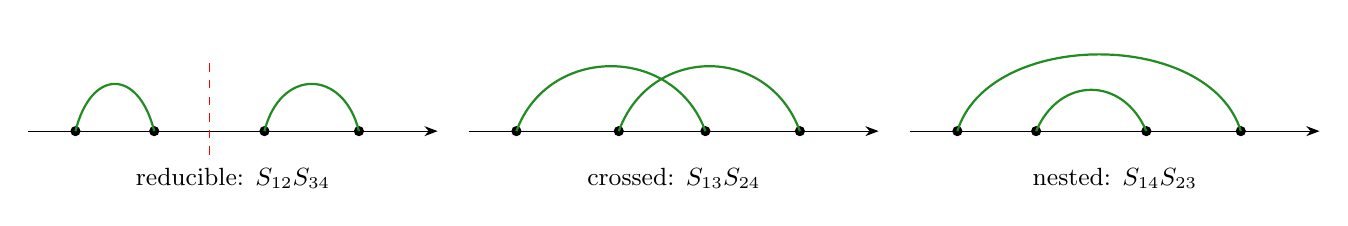
\begin{tikzpicture}[>=Stealth,scale=1.0]
  \tikzset{v/.style={circle,fill=black,inner sep=1.3pt}}
  \draw[->] (0,0)--(5.2,0);
  \foreach \x in {0.6,1.6,3.0,4.2} \node[v] at (\x,0) {};
  \draw[thick,ForestGreen] (0.6,0) .. controls (0.8,0.8) and (1.4,0.8) .. (1.6,0);
  \draw[thick,ForestGreen] (3.0,0) .. controls (3.2,0.8) and (4.0,0.8) .. (4.2,0);
  \draw[dashed,red] (2.3,-0.3)--(2.3,0.9);
  \node[below,font=\small] at (2.6,-0.35) {reducible: $S_{12}S_{34}$};
  \begin{scope}[xshift=5.6cm]
  \draw[->] (0,0)--(5.2,0);
  \foreach \x in {0.6,1.9,3.0,4.2} \node[v] at (\x,0) {};
  \draw[thick,ForestGreen] (0.6,0) .. controls (1.0,1.1) and (2.6,1.1) .. (3.0,0);
  \draw[thick,ForestGreen] (1.9,0) .. controls (2.3,1.1) and (3.8,1.1) .. (4.2,0);
  \node[below,font=\small] at (2.6,-0.35) {crossed: $S_{13}S_{24}$};
  \end{scope}
  \begin{scope}[xshift=11.2cm]
  \draw[->] (0,0)--(5.2,0);
  \foreach \x in {0.6,1.6,3.0,4.2} \node[v] at (\x,0) {};
  \draw[thick,ForestGreen] (0.6,0) .. controls (1.0,1.3) and (3.8,1.3) .. (4.2,0);
  \draw[thick,ForestGreen] (1.6,0) .. controls (1.9,0.7) and (2.7,0.7) .. (3.0,0);
  \node[below,font=\small] at (2.6,-0.35) {nested: $S_{14}S_{23}$};
  \end{scope}
\end{tikzpicture}
\caption{The three fourth-order diagrams.
Time runs to the right; vertices are system superoperators; lines are bath contractions ($S$ or $\chi$).
Only the first can be cut (red) without cutting a line.}
\label{fig:fourth-order}
\end{figure}

\subsection{What the diagrams are good for}

The series \eqref{eq:dyson-super} converges for any finite $t$ but is useless as it stands: at order $2n$ there are $(2n-1)!!$ pairings and the terms grow like $(g^2t^2)^n$.
Every practical method is a \emph{resummation}:
\begin{itemize}[itemsep=1pt]
\item \textbf{Dyson resummation} (\cref{sec:lec5,sec:lec6}): sum the reducible structure exactly and approximate the irreducible kernel.
  This is Nakajima--Zwanzig, and TCL is the same thing organized differently.
\item \textbf{Exponentiation} (\cref{sec:lec7}): when the vertices commute (or are replaced by c-number paths), the pairings exponentiate into an influence functional.
  The noninteracting-blip approximation is a controlled truncation of that exponent.
\item \textbf{Self-consistent resummation} (\cref{sec:lec9}): replace bare propagators by dressed ones inside the kernel (Kadanoff--Baym, GKBA, DMFT-like schemes).
\end{itemize}
In all three, the only input from the bath is the pair $(S,\chi)$, and the only thing that distinguishes the methods is which subset of diagrams is kept and how it is organized.

\subsection{Exercises}

\begin{exercise}\label{ex:4-1}
From the Feynman rules, show that $\Tr_S K^{(2)}(\tau)X=0$ for every $X$ and interpret it.
Show also that $K^{(2)}(\tau)\rho$ is Hermitian for Hermitian $\rho$ (use $(S^\cl)^\dagger=S^\cl$, $(S^\qu)^\dagger=-S^\qu$ and the reality of $S(\tau),\chi(\tau)$).
\end{exercise}

\begin{exercise}\label{ex:4-2}
Derive \cref{eq:K2-bloch}.
(Apply \cref{eq:K2} to each of $\Id,\sx,\sy,\sz$ in turn; the solution writes out the $\sz$ and $\Id$ columns.)
Check the $\theta=0$ and $\theta=\pi/2$ limits against your expectations for pure dephasing and for a damped qubit.
\end{exercise}

\begin{exercise}\label{ex:4-3}
List the $15$ pairings at sixth order and classify them as reducible (cuttable) or irreducible.
How many are irreducible?
(Answer: 10 of the 15 are irreducible if one counts only cuts between consecutive vertices; the reducible ones are products of lower-order irreducible blocks.)
\end{exercise}

\begin{exercise}\label{ex:4-4}
Evaluate $\Gamma(t)$ in \cref{eq:dephasing-exact} for the Lorentzian bath at $T=0$ and show that $\Gamma(t)\simeq 2g^2t^2$ for $t\ll1/\Omega$ (Gaussian decay) and $\Gamma(t)\simeq2S(\omega{=}0)\,t+\text{const}$ for $t\gg1/\gamma$ (exponential decay).
Which value of $S(\omega{=}0)$ enters?
\end{exercise}

\clearpage

%=====================================================================
\section{Lecture 5: Nakajima--Zwanzig, and why the memory kernel is a self-energy}
\label{sec:lec5}

The Nakajima--Zwanzig (NZ) equation is an exact, closed equation of motion for
$\rhoS(t)$. It is derived in five lines with a projection operator, and its memory kernel
$K$ looks at first like a formal object. The content of this lecture is that $K$ is
exactly the sum of the irreducible diagrams of \cref{sec:lec4}, so that the NZ equation is
the Dyson equation of the real-time expansion. We then evaluate $K$ at second order for
the qubit and recover the Bloch--Redfield description, with every rate and shift expressed
through $S$ and $\chi$.

\subsection{The projection and the exact equation}
\label{sec:nz-derivation}

Define the Nakajima--Zwanzig projector~\cite{Nakajima1958,Zwanzig1960}
\begin{equation}
  \Pc X=\rhoB\otimes\Tr_B X,\qquad \Qc=1-\Pc,\qquad \Pc^2=\Pc .
  \label{eq:P}
\end{equation}
$\Pc$ keeps the ``relevant'' part, the reduced state tensored with the fixed reference bath
state. Three facts follow from $[H_B,\rhoB]=0$ and $\avg{B}=0$:
\begin{equation}
  \Pc\Lc_S=\Lc_S\Pc,\qquad \Pc\Lc_B=\Lc_B\Pc=0\ \text{on the range of }\Pc,\qquad \Pc\Lc_I\Pc=0 .
  \label{eq:P-facts}
\end{equation}
(The last one: $\Pc\Lc_I\Pc X=\rhoB\otimes\Tr_B[-i(S B\otimes\rhoB X'-\dots)]\propto\avg{B}=0$.)
Split the von Neumann equation $\dot\rho=\Lc\rho$ into its $\Pc$ and $\Qc$ components:
\begin{equation}
  \partial_t\Pc\rho=\Pc\Lc\Pc\rho+\Pc\Lc\Qc\rho,\qquad
  \partial_t\Qc\rho=\Qc\Lc\Pc\rho+\Qc\Lc\Qc\rho .
\end{equation}
The second is a linear inhomogeneous equation for $\Qc\rho$ with the known source $\Qc\Lc\Pc\rho(s)$:
\begin{equation}
  \Qc\rho(t)=\ee^{\Qc\Lc t}\Qc\rho(0)+\int_0^t\!\dd s\,\ee^{\Qc\Lc(t-s)}\,\Qc\Lc\Pc\rho(s).
\end{equation}
Insert into the first and use \cref{eq:P-facts}:
\begin{equation}
  \boxed{\;\dot\rhoS(t)=\Lc_S\rhoS(t)+\int_0^t\!\dd s\,K(t-s)\,\rhoS(s)+I(t),\qquad
  K(\tau)X=\Tr_B\!\Big[\Lc_I\,\ee^{\Qc\Lc\tau}\,\Qc\Lc_I\big(X\otimes\rhoB\big)\Big],\;}
  \label{eq:NZ}
\end{equation}
with the inhomogeneity $I(t)=\Tr_B[\Lc_I\ee^{\Qc\Lc t}\Qc\rho(0)]$, which vanishes for a
factorized initial state ($\Qc\rho(0)=0$). This is the NZ
equation~\cite[Sec.~9.1]{BreuerPetruccione}. It is exact. Nothing has been assumed about
the strength of the coupling, the Gaussianity of the bath or the size of the system. The
kernel $K(\tau)$ is a superoperator on the system; it depends on $\tau$ only (stationary
bath, time-independent $H$) and it contains the full $\Lc$ inside the exponential, which
is where all the difficulty hides.

\paragraph{Laplace form.}
With $\hat f(z)=\int_0^\infty\dd t\,\ee^{-zt}f(t)$ (Re$\,z>0$), the convolution becomes a product
and \cref{eq:NZ} for the map reads
\begin{equation}
  \boxed{\;\hat\Pi(z)=\frac{1}{z-\Lc_S-\hat K(z)}
  \quad\Longleftrightarrow\quad
  \hat\Pi=\hat\Pi_0+\hat\Pi_0\,\hat K\,\hat\Pi,\qquad \hat\Pi_0=(z-\Lc_S)^{-1}.\;}
  \label{eq:Dyson}
\end{equation}
This is a Dyson equation with $\hat K$ in the role of the self-energy. The next
subsection shows that the analogy is an identity.

\subsection{The kernel is the sum of irreducible diagrams}
\label{sec:nz-irreducible}

\begin{theorem}\label{thm:irreducible}
For the projector \eqref{eq:P}, the NZ kernel is the sum of all diagrams of
\cref{sec:lec4} that cannot be cut between two consecutive vertices without cutting a
line, with the outermost vertices at $0$ and $\tau$:
\begin{equation}
  K(\tau)=\sum_{n\ge1}\;\int_{\tau>t_1>\dots>t_{2n-2}>0}\ \sum_{\text{irreducible pairings of }\{\tau,t_1,\dots,t_{2n-2},0\}}
  \big(\text{vertices}\times\text{lines}\big).
\end{equation}
\end{theorem}

\begin{proof}
Expand $\ee^{\Qc\Lc\tau}$ in powers of $\Lc_I$. Since $\Qc$ commutes with $\Lc_0=\Lc_S+\Lc_B$
(because $\Pc$ does), $\ee^{\Qc\Lc_0s}\Qc=\Qc\ee^{\Lc_0s}$, and the $m$-th order term is
\begin{equation}
  \int_{\tau>s_1>\dots>s_m>0}\Qc\,\ee^{\Lc_0(\tau-s_1)}\,\Qc\Lc_I\,\ee^{\Lc_0(s_1-s_2)}\,\Qc\Lc_I\cdots\Qc\Lc_I\,\ee^{\Lc_0s_m}\,\Qc .
\end{equation}
Sandwiched between the outer $\Tr_B[\Lc_I\cdots]$ and $\Lc_I(X\otimes\rhoB)$, this is the
free (interaction-picture) Wick string of $m+2$ vertices with a factor $\Qc=1-\Pc$ inserted
in every gap between consecutive vertices. Now expand the product of the $(1-\Pc)$'s. A
term with $\Pc$ inserted in a given set $\mathcal C$ of gaps equals, by the definition of
$\Pc$, the Wick string in which the bath is traced and reset to $\rhoB$ at each gap in
$\mathcal C$; by Wick's theorem that is exactly the sum of the pairings in which \emph{no
line crosses any gap in $\mathcal C$}. Hence
\begin{equation}
  \sum_{\mathcal C}(-1)^{|\mathcal C|}\ \#\{\text{pairings with no line across any gap in }\mathcal C\}
  =\#\{\text{pairings with a line across \emph{every} gap}\}
\end{equation}
by inclusion--exclusion, and the right-hand side is the set of irreducible pairings.
\end{proof}

Irreducibility is defined with respect to the reference state $\rhoB$ in $\Pc$: a cut is a
moment at which the bath is \emph{exactly} back in $\rhoB$. A different projector (a
correlated reference state, or Mori's operator projector of \cref{sec:lec8}) gives a
different kernel. The theorem is the real-time version of the statement that the
self-energy is one-particle irreducible; in the superoperator language it goes back to
Schoeller and Sch\"on~\cite{SchoellerSchon1994,Schoeller2000} for fermionic reservoirs and
is the basis of real-time renormalization group methods~\cite{Schoeller2009,Keil2001}; see
also~\cite{LeijnseWegewijs2008,Timm2008} for the explicit comparison with NZ at fourth
order. Two consequences:
\begin{itemize}[itemsep=1pt]
\item $K(0)=K^{(2)}(0)$ exactly: at $\tau=0$ there is no room for internal vertices.
\item $K$ is of order $g^2$ while $\Pi$ is of order $1$; perturbation theory for $K$ is
  perturbation theory for the exponent, which is why NZ at low order already
  captures long-time exponential decay that no finite-order expansion of $\Pi$ can.
\end{itemize}

\subsection{Second order: Born, Redfield, secular, Bloch}
\label{sec:born}

At order $\Lc_I^2$ we drop $\Qc$ in \cref{eq:NZ} (because $\Pc\Lc_I\Pc=0$) and replace
$\ee^{\Qc\Lc\tau}\to\ee^{\Lc_0\tau}$; the result is $K^{(2)}$ of \cref{eq:K2}, now identified as
the first term of the irreducible series. The approximations one layers on top are:
\begin{enumerate}[itemsep=1pt]
\item \textbf{Born (NZ2).} Keep $K\approx K^{(2)}$ in \cref{eq:NZ}, as a time-nonlocal equation.
\item \textbf{Redfield (time-local, nonsecular).} Replace $\rhoS(s)\to\ee^{-\Lc_S(t-s)}\rhoS(t)$
  under the integral (valid when $\rhoS$ changes little, in the interaction picture, over
  the bath correlation time) and extend the upper limit to $\infty$:
  \begin{equation}
    \dot\rhoS=\big[\Lc_S+\Gc^{(2)}_\infty\big]\rhoS,\qquad
    \Gc^{(2)}_\infty=\int_0^\infty\!\dd\tau\,K^{(2)}(\tau)\,\ee^{-\Lc_S\tau}.
    \label{eq:redfield}
  \end{equation}
  This is Redfield's equation~\cite{Redfield1957,WangsnessBloch1953,Bloch1957}; we will
  see in \cref{sec:lec6} that it is the $t\to\infty$ limit of the second-order TCL generator.
\item \textbf{Secular.} Drop the terms of $\Gc^{(2)}_\infty$ that oscillate at $\pm\omega_0$ or $\pm2\omega_0$ in
  the interaction picture. The result is of GKSL form \eqref{eq:GKSL} and generates a
  completely positive semigroup (Davies' theorem~\cite{Davies1974}; see
  \cite[Sec.~3.3.1]{BreuerPetruccione} for the general construction). Without the secular
  step, Redfield can violate positivity at short times.
\end{enumerate}

\begin{exbox}[Example 5.1: the Bloch equations for the qubit]
Apply \cref{eq:redfield} to the kernel \eqref{eq:K2-bloch}. The rotation $\ee^{-\Lc_S\tau}$ acts
on the \emph{input}: $(x_x,x_y)\mapsto(\cos\,x_x+\sin\,x_y,\,-\sin\,x_x+\cos\,x_y)$. Multiplying out
and keeping the secular terms (the $\tau$-integrals of products such as
$S_\tau\cos\omega_0\tau\cos\omega_0\tau$ contain a non-oscillating half; the $cs$ cross terms and
the $\cos^2$-type oscillating halves drop), one finds the Bloch equations
\begin{equation}
  \dot r_z=-\Gamma_1\big(r_z-r_z^{\rm eq}\big),\qquad
  \dot r_\pm=\big(\pm i\tilde\omega_0-\Gamma_2\big)r_\pm,\qquad r_\pm\equiv r_x\pm ir_y ,
  \label{eq:bloch-eqs}
\end{equation}
with
\begin{align}
  \Gamma_1&=\Gamma_\downarrow+\Gamma_\uparrow=2\sin^2\theta\,S(\omega_0),\qquad
  \Gamma_{\downarrow}=2\sin^2\theta\,J(\omega_0)\big[1+n(\omega_0)\big],\quad
  \Gamma_{\uparrow}=2\sin^2\theta\,J(\omega_0)\,n(\omega_0),
  \label{eq:rates-T1}\\
  r_z^{\rm eq}&=-\frac{\chi''(\omega_0)}{S(\omega_0)}=-\tanh\frac{\beta\omega_0}{2},
  \label{eq:rz-eq}\\
  \Gamma_2&=\tfrac12\Gamma_1+\Gamma_\varphi,\qquad \Gamma_\varphi=2\cos^2\theta\,S(\omega{=}0),
  \label{eq:rates-T2}\\
  \tilde\omega_0&=\omega_0+\delta\omega,\qquad
  \delta\omega=2\sin^2\theta\int_0^\infty\!\dd\tau\,S(\tau)\sin\omega_0\tau
  =\frac{\sin^2\theta}{\pi}\,\mathrm P\!\!\int_{-\infty}^{\infty}\!\dd\omega\,\frac{S(\omega)}{\omega_0-\omega}.
  \label{eq:lamb}
\end{align}
Each line is worth a comment.
\begin{itemize}[itemsep=1pt]
\item \Cref{eq:rates-T1}: the population column of $K^{(2)}$ gives
  $\int_0^\infty K_{zz}\dd\tau=-4\sin^2\theta\int_0^\infty S(\tau)\cos\omega_0\tau\,\dd\tau=-2\sin^2\theta S(\omega_0)$. The
  \emph{sum} of the rates is set by the noise at $\omega_0$. Using the FDT,
  $S(\omega_0)=J(\omega_0)[1+2n(\omega_0)]$, which splits into $\Gamma_\downarrow+\Gamma_\uparrow$ as written. This is
  Fermi's golden rule with the $C(\pm\omega_0)$ of \cref{eq:FDT}.
\item \Cref{eq:rz-eq}: the inhomogeneous term is
  $\int_0^\infty K_{z\Id}\dd\tau=-2\sin^2\theta\int_0^\infty\chi(\tau)\sin\omega_0\tau\,\dd\tau=-2\sin^2\theta\,\chi''(\omega_0)$. The
  \emph{difference} of the rates, $\Gamma_\downarrow-\Gamma_\uparrow=2\sin^2\theta\chi''(\omega_0)$, is set by the
  response. The ratio $\chi''/S=\tanh(\beta\omega_0/2)$ is the FDT, and it makes the steady state
  the Gibbs state of $H_S$: detailed balance is the fluctuation--dissipation theorem seen
  from the system. Out of equilibrium (a driven or nonthermal bath), $S$ and $\chi''$ are
  independent and $r_z^{\rm eq}$ defines an effective temperature.
\item \Cref{eq:rates-T2}: pure dephasing samples the noise at zero frequency and
  comes with $\cos^2\theta$; relaxation contributes half its rate to the coherence decay. For
  $S=\sz/2$ one would have $\Gamma_\varphi=\tfrac12\cos^2\theta S(0)$.
\item \Cref{eq:lamb}: the Lamb shift is the Hilbert transform of the \emph{noise} spectrum.
  At $T=0$, $S(\omega)=J(|\omega|)$ and the integral splits into the rotating-wave term
  $\mathrm P\!\int_0^\infty J(\omega)/(\omega_0-\omega)$ and the counter-rotating (Bloch--Siegert) term
  $\int_0^\infty J(\omega)/(\omega_0+\omega)$. The response $\chi'$ drops out of the shift because it is
  even in $\omega$ (\cref{ex:5-2}).
\end{itemize}
For the Lorentzian bath of \cref{sec:lec2} at $T=0$, with $\Omega=\omega_0=1$, $\gamma=0.5$,
$\theta=\pi/4$, $g=0.3$: $\Gamma_\downarrow=0.360$, $\Gamma_\uparrow=0.0055$ (from the negative-frequency
tail), $\Gamma_\varphi=0.0424$, $\Gamma_2=0.225$, $\delta\omega=g^2\sin^2\theta\,\frac{2\Omega}{4\Omega^2+\gamma^2/4}=0.022$. The
script of \cref{sec:numerics} computes $\Gc^{(2)}_\infty$ numerically and reproduces all of these
to three digits (the nonsecular generator gives a precession frequency $1.0219$ versus
$1.0222$ secular).
\end{exbox}

\begin{figure}[t]
\centering
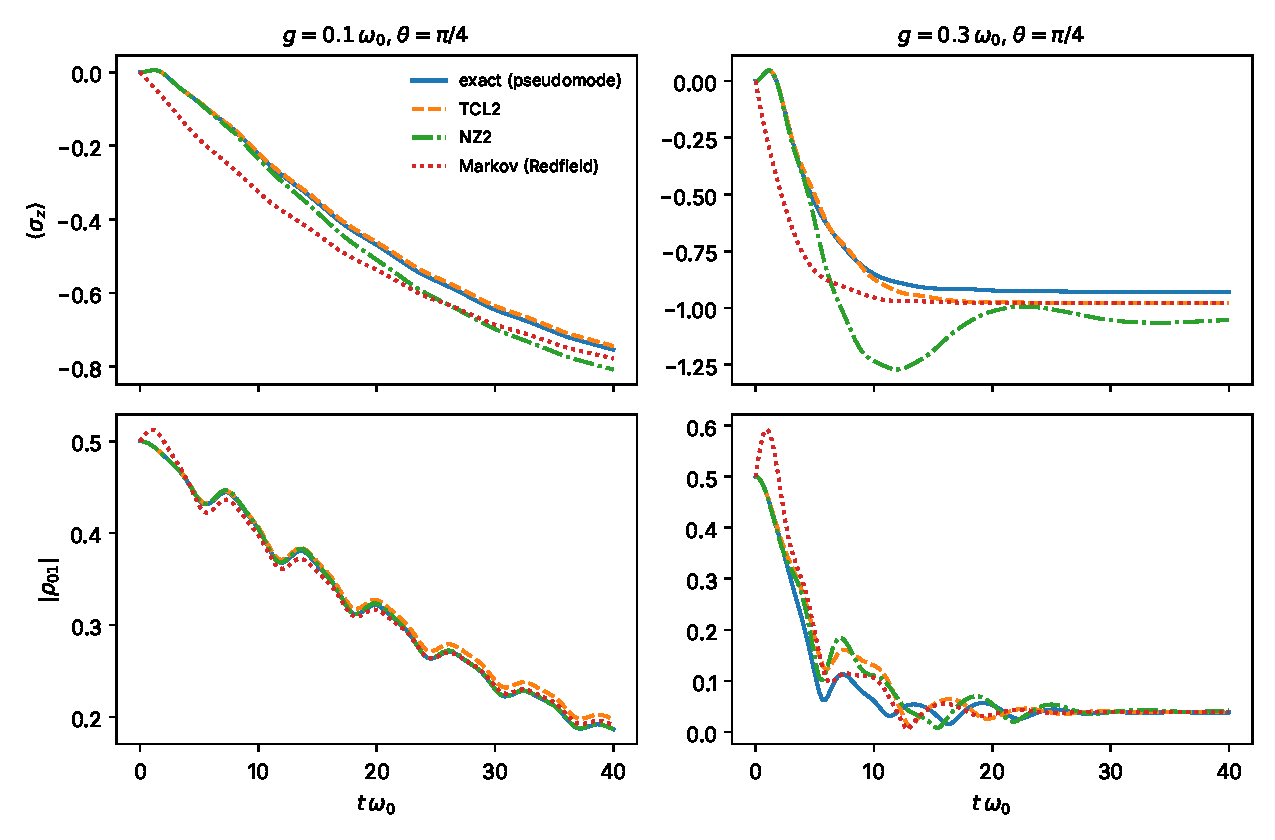
\includegraphics[width=\textwidth]{figures/fig_dynamics.pdf}
\caption{Qubit dynamics in the Lorentzian bath ($\Omega=\omega_0$, $\gamma=0.5\omega_0$, $T=0$,
$\theta=\pi/4$), starting from $\ket{+x}$, for weak (left) and moderate (right) coupling. Exact
(pseudomode) versus the three second-order schemes of this lecture and the next: NZ2
(Born, time-nonlocal), TCL2 (time-local, time-dependent rates) and the Markovian Redfield
limit. At $g=0.3$ the Born kernel drives $\avg{\sz}$ below $-1$, a violation of positivity;
TCL2 stays physical and tracks the exact solution; Markov misses the initial slip and the
coupling-induced shift of the steady state.}
\label{fig:dynamics}
\end{figure}

\Cref{fig:dynamics} compares the three second-order schemes with the exact solution.
Three lessons: (i) at weak coupling all agree, and the Markovian rates of Example~5.1 are
quantitatively right after a transient of duration $\sim1/\gamma$; (ii) the Born kernel used
\emph{nonlocally} (NZ2) is the \emph{worst} of the three at stronger coupling, overshooting
to unphysical states, a well-known pathology~\cite{SmirneVacchini2010}; (iii) the exact
steady state is not the Gibbs state of $H_S$ but the reduced state of the global
equilibrium, which the second-order schemes can only approximate.

\subsection{Beyond second order}

The fourth-order kernel is the sum of the crossed and nested diagrams of
\cref{fig:fourth-order}, each with its full vertex structure (all assignments of
$\cl/\qu$ consistent with the rules, i.e.\ $\qu\qu$ lines carrying $S$ and $\qu\cl$ lines
carrying $-i\chi$). Written out,
\begin{equation}
  K^{(4)}(\tau)=\int_{\tau>t_1>t_2>0}\Big\{V_\tau V_{t_1}V_{t_2}V_0\Big\}_{\text{crossed }(\tau t_2)(t_10)}
  +\Big\{V_\tau V_{t_1}V_{t_2}V_0\Big\}_{\text{nested }(\tau0)(t_1t_2)},
\end{equation}
where $V_{t}$ denotes the vertex at time $t$ (either $-iS^\qu$ or $-iS^\cl$ according to the
line it belongs to),
with free propagators between vertices in the Schr\"odinger picture. For
$\theta=0$ on the coherence it reduces to the crossed and nested integrals of
\cref{eq:dephasing-4th} times $16$. Explicit fourth-order kernels for the spin-boson model
were worked out in the TCL form by Breuer, Kappler and
Petruccione~\cite{BreuerKapplerPetruccione2001}; in the NZ form the bookkeeping is easiest
in Laplace space~\cite{Timm2008}. \Cref{fig:kernels} (left) shows the exact kernel of the
Lorentzian model, extracted numerically from the pseudomode representation as
$\Pc\Lc_I\ee^{\Qc\Lc\tau}\Qc\Lc_I\Pc$, against $K^{(2)}$: the higher orders shift the oscillation
frequency inside the kernel (a self-consistent Lamb shift) and change its damping, but
$K(0)=K^{(2)}(0)$ exactly, as the theorem requires.

\begin{figure}[t]
\centering
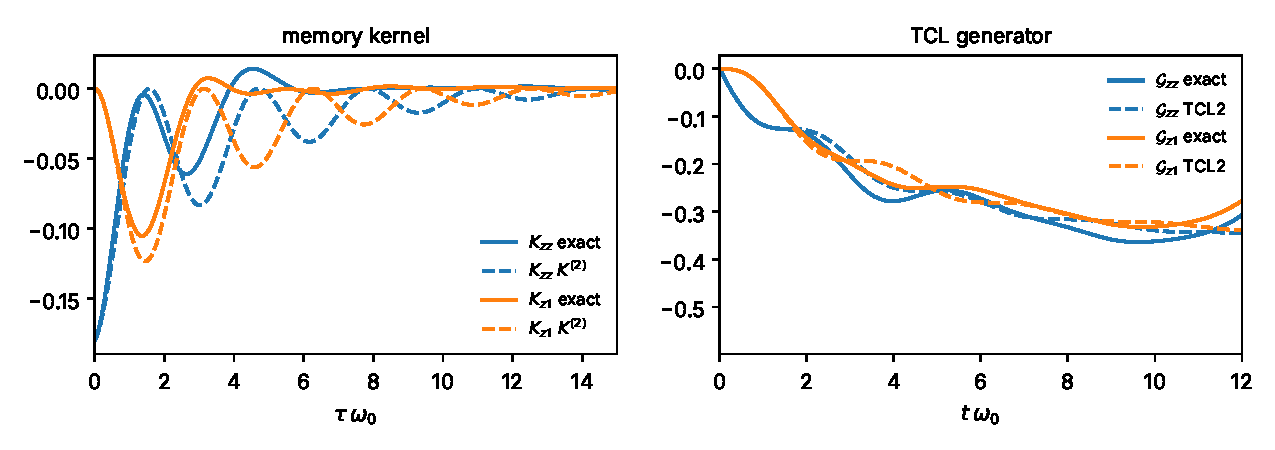
\includegraphics[width=\textwidth]{figures/fig_kernels.pdf}
\caption{Left: the exact NZ memory kernel of the Lorentzian model at $g=0.3$,
$\theta=\pi/4$ (elements $K_{zz}$ and $K_{z\Id}$ in the Bloch basis), compared with the Born
kernel $K^{(2)}$. Right: the exact TCL generator $\Gc(t)=\dot\Pi\Pi^{-1}-\Lc_S$ compared
with the TCL2 generator $\Gc^{(2)}(t)$ (\cref{sec:lec6}). Both agree at short times by
construction; the exact generator develops large excursions near $t\omega_0\approx12$ where
$\Pi(t)$ becomes nearly singular.}
\label{fig:kernels}
\end{figure}

\subsection{Correlated initial states and the inhomogeneity}

If $\rho(0)$ is not factorized, $I(t)$ in \cref{eq:NZ} is nonzero. It decays on the bath
correlation time if the initial correlations are short-ranged, and it can be absorbed
into a modified kernel in some cases. In the Keldysh language the same information lives
on the imaginary-time (Matsubara) branch attached to the contour at
$t=0$~\cite[Ch.~4]{StefanucciVanLeeuwen}. One should not expect $\Pi(t)$ to be a
completely positive map of $\rhoS(0)$ in that case~\cite{Pechukas1994}.

\subsection{Exercises}

\begin{exercise}\label{ex:5-1}
Carry out the derivation of \cref{eq:NZ} with a general projector $\Pc$ (not necessarily
of the form \eqref{eq:P}) and identify which steps use $\Pc\Lc_I\Pc=0$ and $[\Pc,\Lc_0]=0$. What
changes if $\avg{B}\ne0$? (Hint: absorb $S\avg{B}$ into $H_S$.)
\end{exercise}

\begin{exercise}\label{ex:5-2}
Derive the Bloch equations \eqref{eq:bloch-eqs}--\eqref{eq:lamb} from \cref{eq:K2-bloch}.
Show that the real part of the response, $\chi'$, cancels from $\delta\omega$ and explain why
with a parity argument. Then obtain the same rates from the operator form
$\Gc X=-i[H_S+H_{\rm LS},X]+\sum_\omega\gamma(\omega)\big(A(\omega)XA(\omega)^\dagger-\tfrac12\{A(\omega)^\dagger A(\omega),X\}\big)$ with
$A(\pm\omega_0)=\sin\theta\,\sigma_\mp$, $A(0)=\cos\theta\,\sz$, $\gamma(\omega)=C(\omega)$~\cite[Sec.~3.3.1]{BreuerPetruccione}.
\end{exercise}

\begin{exercise}\label{ex:5-3}
Show that the secular generator of \cref{ex:5-2} is of GKSL form with
$L_1=\sigma_-$, $L_2=\sigma_+$, $L_3=\sz$ and nonnegative rates. Then take the nonsecular
Redfield generator for $\theta=\pi/2$ and find an initial state and a time at which
$\Tr\rhoS^2>1$ for a Lorentzian bath with $\gamma\gtrsim\omega_0$.
\end{exercise}

\begin{exercise}\label{ex:5-4}
Prove $K(0)=K^{(2)}(0)$ directly from \cref{eq:NZ}. Then show that in Laplace space
$\hat K(z)=z-\Lc_S-\hat\Pi(z)^{-1}$, so that the exact kernel can be \emph{extracted} from the
exact map (this is the route of Shi and Geva~\cite{ShiGeva2003} and of Cohen and
Rabani~\cite{CohenRabani2011}). Use it to show that for pure dephasing ($\theta=0$) the
coherence kernel $\hat K_{01}(z)$ is an infinite series in $g^2$ even though the exact
solution \eqref{eq:dephasing-exact} is ``second order'' in a different sense.
\end{exercise}

\clearpage

%=====================================================================
\section{Lecture 6: Time-convolutionless equations and the NZ--TCL map}
\label{sec:lec6}

A time-nonlocal equation is exact but awkward: it needs the whole history of $\rhoS$, and
its truncations behave badly (\cref{fig:dynamics}). The time-convolutionless (TCL)
technique~\cite{Shibata1977,Chaturvedi1979,HanggiTalkner1977} trades the convolution for
a time-dependent generator, $\dot\rhoS=\Gc(t)\rhoS(t)$. This lecture derives it, computes it for
the qubit, shows how it is related to the NZ kernel, and discusses when it fails.

\subsection{Derivation}

Work in the interaction picture, $\dot{\tilde\rho}=\tilde\Lc_I(t)\tilde\rho$, and let
$\tilde G(t,s)$ be the full propagator from $s$ to $t$ (so $\tilde\rho(t)=\tilde G(t,s)\tilde\rho(s)$)
and $\tilde G(t,s)^{-1}=\tilde G(s,t)$ the backward propagator. The trick is to express the
\emph{past} in terms of the \emph{present}: $\tilde\rho(s)=\tilde G(s,t)\tilde\rho(t)$. Start from
the $\Qc$-equation solved as in \cref{sec:nz-derivation},
\begin{equation}
  \Qc\tilde\rho(t)=\hat G(t,0)\Qc\tilde\rho(0)+\int_0^t\!\dd s\,\hat G(t,s)\,\Qc\tilde\Lc_I(s)\,\Pc\,\tilde\rho(s),
  \qquad \hat G(t,s)=T\exp\Big[\int_s^t\!\Qc\tilde\Lc_I\Big],
\end{equation}
and substitute $\tilde\rho(s)=\tilde G(s,t)[\Pc+\Qc]\tilde\rho(t)$. Defining
\begin{equation}
  \Sigma(t)\equiv\int_0^t\!\dd s\,\hat G(t,s)\,\Qc\tilde\Lc_I(s)\,\Pc\,\tilde G(s,t),
\end{equation}
which is of order $\Lc_I$ and vanishes at $t=0$, we get $[1-\Sigma(t)]\Qc\tilde\rho(t)=\hat G(t,0)\Qc\tilde\rho(0)+\Sigma(t)\Pc\tilde\rho(t)$.
Wherever $1-\Sigma(t)$ is invertible (certainly for short times or weak coupling),
\begin{equation}
  \boxed{\;\partial_t\Pc\tilde\rho(t)=\tilde\Gc(t)\,\Pc\tilde\rho(t)+\tilde I(t),\qquad
  \tilde\Gc(t)=\Pc\tilde\Lc_I(t)\big[1-\Sigma(t)\big]^{-1}\Pc,\;}
  \label{eq:TCL}
\end{equation}
with $\tilde I(t)=\Pc\tilde\Lc_I(t)[1-\Sigma(t)]^{-1}\hat G(t,0)\Qc\tilde\rho(0)$, zero for factorized initial
states~\cite[Sec.~9.2]{BreuerPetruccione}. The equation is exact, time-local, and its
generator has a perturbative expansion obtained by expanding $[1-\Sigma]^{-1}=\sum_n\Sigma^n$:
\begin{align}
  \tilde\Gc^{(2)}(t)&=\int_0^t\!\dd t_1\,\Pc\tilde\Lc_I(t)\tilde\Lc_I(t_1)\Pc ,
  \label{eq:TCL2}\\
  \tilde\Gc^{(4)}(t)&=\int_0^t\!\dd t_1\!\int_0^{t_1}\!\dd t_2\!\int_0^{t_2}\!\dd t_3\,
  \Big[\avg{\tilde\Lc_I(t)\tilde\Lc_I(t_1)\tilde\Lc_I(t_2)\tilde\Lc_I(t_3)}
  -\avg{\tilde\Lc_I(t)\tilde\Lc_I(t_1)}\avg{\tilde\Lc_I(t_2)\tilde\Lc_I(t_3)}\notag\\
  &\hspace{3.2cm}-\avg{\tilde\Lc_I(t)\tilde\Lc_I(t_2)}\avg{\tilde\Lc_I(t_1)\tilde\Lc_I(t_3)}
  -\avg{\tilde\Lc_I(t)\tilde\Lc_I(t_3)}\avg{\tilde\Lc_I(t_1)\tilde\Lc_I(t_2)}\Big],
  \label{eq:TCL4}
\end{align}
where $\avg{\cdots}\equiv\Pc\cdots\Pc$ restricted to the system (the ``ordered cumulants'' of
van Kampen; see \cite[Sec.~9.2.4]{BreuerPetruccione} and
\cite{BreuerKapplerPetruccione2001}). Compare with the fourth-order NZ kernel: there, only
the \emph{reducible} pairing $(t\,t_1)(t_2t_3)$ is subtracted (by the $\Qc$'s), while here all
three products of pair contractions are subtracted, including the crossed and nested
ones. TCL4 is \emph{not} NZ4 with the convolution removed; it is a different
reorganization, which happens to contain NZ4 plus terms generated by the time-locality.

\subsection{TCL2 for the qubit: time-dependent rates}

In the Schr\"odinger picture, \cref{eq:TCL2} reads
\begin{equation}
  \dot\rhoS=\big[\Lc_S+\Gc^{(2)}(t)\big]\rhoS(t),\qquad
  \Gc^{(2)}(t)=\int_0^t\!\dd\tau\,K^{(2)}(\tau)\,\ee^{-\Lc_S\tau},
  \label{eq:TCL2-S}
\end{equation}
i.e.\ Redfield's generator \eqref{eq:redfield} with the upper limit at $t$ instead of
$\infty$. All the Markovian rates of Example~5.3 become running integrals:

\begin{exbox}[Example 6.1: the running rates]
Repeating the secular reduction of Example~5.3 with $\int_0^t$ instead of $\int_0^\infty$,
\begin{align}
  \Gamma_1(t)&=4\sin^2\theta\int_0^t\!\dd\tau\,S(\tau)\cos\omega_0\tau ,&
  \Gamma_1(t)\,r_z^{\rm eq}(t)&=-2\sin^2\theta\int_0^t\!\dd\tau\,\chi(\tau)\sin\omega_0\tau,\notag\\
  \Gamma_\varphi(t)&=4\cos^2\theta\int_0^t\!\dd\tau\,S(\tau),&
  \delta\omega(t)&=2\sin^2\theta\int_0^t\!\dd\tau\,S(\tau)\sin\omega_0\tau .
  \label{eq:running-rates}
\end{align}
Three features are general. (i) All rates vanish at $t=0$ as $t^1$ (since $K(0)\ne0$):
decay is initially quadratic in time, the Zeno regime. (ii) They approach their Markov
values on the bath correlation time $\tau_B$ ($=2/\gamma$ for the Lorentzian, $1/\omega_c$ or
$1/\pi T$ for the Ohmic bath). (iii) In between they can \emph{overshoot} and even become
negative: for the Lorentzian bath, $\Gamma_1(t)\propto\int_0^tS(\tau)\cos\omega_0\tau\,\dd\tau$ with
$S(\tau)\cos\omega_0\tau=\tfrac{g^2}2\ee^{-\gamma\tau/2}[1+\cos2\omega_0\tau]$ at resonance is monotonic, but
$\Gamma_\varphi(t)\propto\int_0^tS(\tau)\dd\tau=g^2\int_0^t\ee^{-\gamma\tau/2}\cos\Omega\tau\,\dd\tau$ oscillates and is
negative in windows when $\Omega>\gamma/2$. A negative rate in a time-local generator is the
standard signature of information flowing back from the bath~\cite{deVega2017}.
\end{exbox}

For pure dephasing ($\theta=0$) TCL2 is \emph{exact}: the generator on the coherence is
$-i\omega_0-\dot\Gamma(t)$ with $\Gamma$ of \cref{eq:dephasing-exact}, and $\dot\Gamma(t)=4\int_0^tS(\tau)\dd\tau=\Gamma_\varphi(t)$.
All higher ordered cumulants \eqref{eq:TCL4} vanish because the vertices commute and the
full fourth-order moment equals the sum of the three pair products. This is the cleanest
demonstration that ``order $n$'' means different things in different schemes: the same
model is second order in TCL and infinite order in NZ (Exercise~\ref{ex:5-4}).

\subsection{The NZ--TCL map}

Both equations describe the same map, so the kernel and the generator determine each
other. Writing the NZ equation for $\Pi(t)$ and multiplying by $\Pi(t)^{-1}$,
\begin{equation}
  \boxed{\;\Gc(t)=\Lc_S+\int_0^t\!\dd s\,K(t-s)\,\Pi(s)\,\Pi(t)^{-1},\qquad
  \Gc(t)=\dot\Pi(t)\Pi(t)^{-1},\;}
  \label{eq:TCLNZ}
\end{equation}
an exact relation wherever $\Pi(t)$ is invertible~\cite{ChruscinskiKossakowski2010}.
Conversely, given $\Gc$ one reconstructs $\Pi=T\exp\int\Gc$ and then $K$ from the Laplace
relation of Exercise~\ref{ex:5-4}. Nestmann, Bruch and Wegewijs~\cite{Nestmann2021} turned
\cref{eq:TCLNZ} into a fixed-point iteration, $\Gc\mapsto\Lc_S+\int K(t-s)\,T\ee^{\int_t^s\Gc}\dd s$, that
converges to the exact generator and makes explicit how a time-nonlocal kernel
``generates'' a time-local evolution: the generator at time $t$ is the kernel averaged over
the past with the propagator as weight. Inserting $K\approx K^{(2)}$ and $\Pi\approx\Pi_0$ gives
back $\Gc^{(2)}$; inserting $K^{(2)}+K^{(4)}$ with $\Pi$ to the required order reproduces
\cref{eq:TCL4} and exhibits the extra subtractions as the $\Pi^{(2)}\Pi_0^{-1}$ corrections
(Exercise~\ref{ex:6-3}). Reimer \emph{et al.}~\cite{Reimer2019} compare these and three further exact
formulations with attention to complete positivity and divisibility.

\subsection{When the generator does not exist}
\label{sec:tcl-singular}

$\Gc(t)$ is defined only where $\Pi(t)$ is invertible. For the transverse model
($\theta=\pi/2$) in the rotating-wave approximation and a Lorentzian bath at $T=0$, the
single-excitation sector is exactly solvable: the excited amplitude obeys
$\ddot c_e+\tfrac\gamma2\dot c_e+g^2c_e=0$ at resonance, so
\begin{equation}
  c_e(t)=\ee^{-\gamma t/4}\Big[\cosh\tfrac{dt}{4}+\tfrac{\gamma}{d}\sinh\tfrac{dt}{4}\Big],\qquad d=\sqrt{\gamma^2-16g^2},
\end{equation}
and $\rho_{ee}(t)=|c_e(t)|^2\rho_{ee}(0)$, $\rho_{eg}(t)=c_e(t)\rho_{eg}(0)$. The exact generator is of
GKSL form with the single time-dependent rate $\gamma(t)=-2\Re[\dot c_e/c_e]$ and shift
$-2\Im[\dot c_e/c_e]$~\cite[Sec.~10.1]{BreuerPetruccione,Vacchini2010}. For $16g^2>\gamma^2$ the
amplitude oscillates and crosses zero at finite times ($t\approx7.3/\omega_0$ for our $g=0.3$,
$\gamma=0.5$), where $\gamma(t)\to\infty$: the map is still perfectly well defined and
completely positive, but it is not invertible, and no time-local generator exists there.
The NZ kernel has no such problem. ``Local versus nonlocal'' is therefore a statement
about the representation, not about the physics~\cite{ChruscinskiKossakowski2010}.
Without the rotating-wave approximation the zero of $c_e$ is lifted (the counter-rotating
and $\sz$ terms feed the coherence from other components), but the near-singularity
survives as the large excursion of the exact generator in \cref{fig:kernels} (right) near
$t\omega_0\approx12$, where the smallest singular value of $\Pi(t)$ drops to $10^{-2}$.

\subsection{What to take from the numerical figures}

\Cref{fig:dynamics,fig:kernels} illustrate a hierarchy that holds quite generally for
Gaussian baths and weak-to-moderate coupling: Markov $<$ NZ2 $\lesssim$ TCL2 in
accuracy at short times, and Markov $\approx$ TCL2 $>$ NZ2 at long times, with NZ2 prone to
unphysical overshoots. The reason is structural: TCL2 is exact to second order in the
coupling \emph{for the generator}, and errors in the generator stay bounded; NZ2 is exact
to second order for the kernel but the convolution with the exact history amplifies the
missing fourth-order terms. Smirne and Vacchini~\cite{SmirneVacchini2010} give a careful
side-by-side for the two-level system; the lesson has been known since the early
comparisons of the two schemes in chemical physics (see the references in
\cite{BreuerKapplerPetruccione2001}).

\subsection{Exercises}

\begin{exercise}\label{ex:6-1}
Show that $\Sigma(0)=0$, that $\Sigma$ is of first order in $\Lc_I$, and derive
\cref{eq:TCL2,eq:TCL4} from \cref{eq:TCL}. Explain why odd orders vanish.
\end{exercise}

\begin{exercise}\label{ex:6-2}
Evaluate the running rates \eqref{eq:running-rates} in closed form for the Lorentzian bath
at $T=0$ and find the time windows in which $\Gamma_\varphi(t)<0$. Plot $\Gamma_\varphi(t)$, $\Gamma_1(t)$ and
$r_z^{\rm eq}(t)$ for the parameters of \cref{fig:dynamics} and compare with the script's output.
\end{exercise}

\begin{exercise}\label{ex:6-3}
Expand \cref{eq:TCLNZ} to fourth order using $\Pi=\Pi_0+\Pi^{(2)}+\dots$ and $K=K^{(2)}+K^{(4)}+\dots$,
and show that the extra terms relative to $\int K^{(4)}\Pi_0\Pi_0^{-1}$ are exactly the
crossed and nested subtractions in \cref{eq:TCL4}.
\end{exercise}

\begin{exercise}\label{ex:6-4}
For the rotating-wave model of \cref{sec:tcl-singular}, compute the exact NZ kernel
$\hat K_{ee}(z)$ for the population and show that it is finite and analytic for
$\Re z>-\gamma/4$ even when $c_e$ has zeros. Where are the singularities of
$\hat\Gc$, if one tries to define it by Laplace transform?
\end{exercise}

\clearpage

%=====================================================================
\section{Lecture 7: Path integrals: the influence functional, the polaron frame and NIBA}
\label{sec:lec7}

So far we have organized the perturbation series by what the bath does to the
\emph{system superoperators}. The path integral does the opposite: it replaces the system
operators by c-number paths, so that the bath can be integrated out \emph{exactly} into
an exponential, the Feynman--Vernon influence functional~\cite{FeynmanVernon1963}. For a
qubit the paths are discrete, which leads to the blip--sojourn expansion of Leggett
\emph{et al.}~\cite{Leggett1987} and to the noninteracting-blip approximation (NIBA), the
workhorse of the dissipative two-level system. We show that NIBA is nothing but the
second-order Nakajima--Zwanzig kernel in the polaron frame.

\subsection{The influence functional as Wick's theorem with a commutative system}
\label{sec:FV-derivation}

Suppose the system superoperators at different times commuted. Then the sum over all
pairings of $2n$ vertices would be $\frac{1}{n!}$ times the $n$-th power of the single
contraction, and the whole Dyson series \eqref{eq:dyson-super} would exponentiate.
Operators do not commute, but in a path integral they are replaced by c-number paths: on
the forward branch $S\to s^+(t)$, on the backward branch $S\to s^-(t)$, and in rotated
variables $s^\cl=\frac12(s^++s^-)$, $s^\qu=s^+-s^-$. Repeating \cref{sec:feynman-rules} with
c-number vertices, the sum over pairings exponentiates to
\begin{equation}
  \boxed{\;
  \Phi[s^\cl,s^\qu]=-\int_0^t\!\dd t_1\!\int_0^{t_1}\!\dd t_2\,
  \Big[s^\qu(t_1)\,S(t_1-t_2)\,s^\qu(t_2)-i\,s^\qu(t_1)\,\chi(t_1-t_2)\,s^\cl(t_2)\Big],\;}
  \label{eq:FV}
\end{equation}
and the reduced density matrix is
\begin{equation}
  \rhoS(t)=\int\!\mathcal Ds^+\mathcal Ds^-\;\ee^{\,iA_S[s^+]-iA_S[s^-]+\Phi[s^\cl,s^\qu]}\;(\text{boundary terms}),
\end{equation}
with $A_S$ the system action. In the original $\pm$ variables and with $C=S-\tfrac i2\chi$,
\cref{eq:FV} is Feynman and Vernon's
$\Phi=-\int_{t_1>t_2}\big(s^+_1-s^-_1\big)\big[C(t_1-t_2)s^+_2-C^*(t_1-t_2)s^-_2\big]$, which the reader should
check (\cref{ex:7-1}). The rotated form \cref{eq:FV} says: the \emph{noise} kernel couples
the quantum path to itself, the \emph{response} kernel couples the quantum path to the
earlier classical path, and there is no $\cl$--$\cl$ term. Equivalently,
$\Phi=-\frac12\int\!\!\int s^aD^{ab}s^b$ with $D$ the Larkin--Ovchinnikov matrix \eqref{eq:LO}: this is
how the influence functional appears when a Gaussian bath is integrated out of the
Keldysh action~\cite[Sec.~3.2]{Kamenev2011}, \cite[Secs.~3--4]{Grabert1988},
\cite[Ch.~5]{Weiss2012}. For a single Gaussian bath, \cref{eq:FV} contains \emph{all} the
information that any method uses; they differ only in how they handle the
non-commutativity that the path integral pushes into the measure.

\begin{exbox}[Example 7.1: reading the influence functional]
\emph{(i) Pure dephasing.} With $S=\sz$ and the system restricted to the coherence
$\ket0\bra1$, the path variables are frozen at $s^+=+1$, $s^-=-1$, so $s^\cl=0$ and $s^\qu=2$. Then
$\Phi=-4\int_{t_1>t_2}S(t_1-t_2)=-\Gamma(t)$ and $\rho_{01}(t)=\rho_{01}(0)\ee^{-i\omega_0t-\Gamma(t)}$,
reproducing \cref{eq:dephasing-exact} in one line. The coherence is a path on which the
two branches maximally disagree, and only the noise sees it.

\emph{(ii) Semiclassical limit and Langevin equation.} $\Phi$ is at most quadratic in
$s^\qu$. Decouple the quadratic term with an auxiliary real field $\xi$ (Hubbard--Stratonovich),
$\exp[-\tfrac12\!\int\!\!\int s^\qu Ss^\qu]=\int\!\mathcal D\xi\,
\exp[-\tfrac12\!\int\!\!\int\xi S^{-1}\xi+i\!\int\!\xi s^\qu]$, and expand the system action to
first order in $s^\qu$ (exact for a harmonic system). The $s^\qu$ integral then produces a
delta functional enforcing an equation of motion for $s^\cl$ with damping kernel $\chi$ and
a Gaussian force $\xi$ of correlator $S$: the quantum Langevin
equation~\cite{FordKacMazur1965,CaldeiraLeggett1983}. The $\qu$ field has become the
Martin--Siggia--Rose response field~\cite{MartinSiggiaRose1973}, the $\qu\qu=0$ rule of
\cref{eq:LO} is the statement that the response field has no self-correlation
(causality), and in the high-temperature limit $S(\omega)\to2T\chi''(\omega)/\omega$ is the classical
FDT~\cite[Ch.~4]{Kamenev2011}. \Cref{sec:lec8} returns to this from Mori's side.
\end{exbox}

\subsection{Spin paths: blips and sojourns}

For a qubit there is no continuous coordinate, but \cref{eq:FV} still applies if we
expand in the part of $H_S$ that does not commute with $S$. Use the Leggett form
\eqref{eq:leggett-form}: $S=\sz'$ is diagonal, the bias $\varepsilon$ is diagonal, and the
tunnelling $-\tfrac\Delta2\sx'$ flips the spin. Expanding $\ee^{-iHt}$ and $\ee^{iHt}$ in $\Delta$,
each branch becomes a piecewise-constant path $s^\pm(t)=\pm1$ with flips at the vertices
(a factor $i\Delta/2$ each, and the bias phase $\ee^{\mp i\varepsilon s^\pm\dd t/2}$ along the way). The
pair $(s^+,s^-)$ then alternates between \emph{sojourns}, $s^+=s^-$ (so $s^\qu=0$, $s^\cl=\pm1$),
and \emph{blips}, $s^+=-s^-$ (so $s^\qu=\pm2$, $s^\cl=0$)~\cite[Sec.~IV]{Leggett1987}, \cite[Ch.~21]{Weiss2012}.
In Keldysh language a sojourn is a segment where the two branches agree, a classical
configuration, and a blip is where they differ, a quantum excursion. Inserting such
paths in \cref{eq:FV}, two integrations by parts convert the kernels into the functions
\begin{equation}
  Q_2(\tau)=\frac4\pi\int_0^\infty\!\dd\omega\,\frac{J(\omega)}{\omega^2}\coth\tfrac{\beta\omega}2\,(1-\cos\omega\tau),\qquad
  Q_1(\tau)=\frac4\pi\int_0^\infty\!\dd\omega\,\frac{J(\omega)}{\omega^2}\sin\omega\tau,
  \label{eq:Q12}
\end{equation}
with $\ddot Q_2=4S$ and $\ddot Q_1=-2\chi$ for $\tau>0$ (the factor 4 is again ``$\sz$ versus
$\sz/2$''; with Leggett's coupling the prefactor is $1/\pi$). The influence functional
becomes a sum of pairwise interactions: blip--blip through $Q_2$ (noise), and
blip--sojourn through $Q_1$ (response), with the sojourn \emph{preceding} the blip, as
causality requires.

\begin{keybox}[The noninteracting-blip approximation]
Keep, for each blip of duration $\tau$, only its self-interaction $\ee^{-Q_2(\tau)}$ and its
interaction with the immediately preceding sojourn, $\ee^{\mp iQ_1(\tau)}$; drop all
interactions between different blips and between a blip and earlier sojourns. The
resulting series for the population $P(t)\equiv\avg{\sz'}_t$ sums to the integro-differential
equation
\begin{equation}
  \boxed{\;\dot P(t)=-\int_0^t\!\dd\tau\Big[K^s(\tau)\,P(t-\tau)+K^a(\tau)\Big],\qquad
  \begin{aligned}
  K^s(\tau)&=\Delta^2\,\ee^{-Q_2(\tau)}\cos Q_1(\tau)\cos\varepsilon\tau,\\
  K^a(\tau)&=\Delta^2\,\ee^{-Q_2(\tau)}\sin Q_1(\tau)\sin\varepsilon\tau .
  \end{aligned}\;}
  \label{eq:NIBA}
\end{equation}
\end{keybox}
This is the NIBA of Leggett \emph{et al.}~\cite[Sec.~V]{Leggett1987}; see
\cite[Ch.~21]{Weiss2012} for its many extensions. It is exact to leading order in $\Delta$;
it is also exact for the Ohmic bath at $\alpha=\tfrac12$ (Toulouse) and very accurate at
high temperature or strong damping, where blips are short and dilute. It fails for a
biased system at low temperature and weak damping, where the long-time Boltzmann
weights come out wrong (\cref{ex:7-4}); the reason will be transparent below.

\subsection{NIBA is the second-order NZ kernel in the polaron frame}

The blip language suggests a unitary transformation: a blip is a segment in which the
bath is displaced in opposite directions on the two branches. Displace it once and for
all with the polaron transformation~\cite{SilbeyHarris1984}
\begin{equation}
  U=\exp\Big[-\sz'\sum_k\frac{g_k}{\omega_k}\big(b_k^\dagger-b_k\big)\Big],\qquad
  U^\dagger b_kU=b_k-\sz'\frac{g_k}{\omega_k},
\end{equation}
which gives $U^\dagger(H_B+\sz'B)U=H_B-\sum_kg_k^2/\omega_k$: the diagonal coupling is removed
at the price of dressing the tunnelling,
\begin{equation}
  H'=U^\dagger HU=\frac{\varepsilon}{2}\sz'+H_B-\frac{\Delta}{2}\big(\sigma_+'B_++\sigma_-'B_-\big)+\text{const},\qquad
  B_\pm=\exp\Big[\pm2\sum_k\frac{g_k}{\omega_k}\big(b_k^\dagger-b_k\big)\Big].
  \label{eq:polaron-H}
\end{equation}
Now treat $V=-\tfrac\Delta2(\sigma_+'B_++\sigma_-'B_-)$ as the perturbation and use the NZ equation
with Zwanzig's \emph{diagonal} projector $\Pc_dX=\sum_{i=\uparrow\downarrow}\ket i\bra i\otimes\rhoB\,\Tr_B\bra iX\ket i$,
which keeps only the populations. Since $V$ is off-diagonal, $\Pc_dV\Pc_d=0$ exactly and the
second-order kernel needs no $\Qc$:
\begin{equation}
  \dot P_\uparrow(t)=\int_0^t\!\dd\tau\Big[w_{\uparrow\leftarrow\downarrow}(\tau)P_\downarrow(t-\tau)-w_{\downarrow\leftarrow\uparrow}(\tau)P_\uparrow(t-\tau)\Big],
  \qquad w_{\uparrow\leftarrow\downarrow}(\tau)=\frac{\Delta^2}{2}\Re\Big[\ee^{i\varepsilon\tau}\avg{B_-(0)B_+(\tau)}\Big],
\end{equation}
and $w_{\downarrow\leftarrow\uparrow}(\tau)=\frac{\Delta^2}2\Re[\ee^{-i\varepsilon\tau}\avg{B_+(0)B_-(\tau)}]$. The dressing operators
are displacement operators, and the thermal expectation of a product of two
displacements is a Gaussian (\cref{ex:7-3}):
\begin{equation}
  \avg{B_-(0)B_+(\tau)}=\avg{B_+(0)B_-(\tau)}=\ee^{-Q_2(\tau)+iQ_1(\tau)},
  \label{eq:FC}
\end{equation}
with exactly the $Q_{1,2}$ of \cref{eq:Q12}. Hence
$w_{\downarrow\leftarrow\uparrow}=\tfrac{\Delta^2}2\ee^{-Q_2}\cos(\varepsilon\tau-Q_1)$,
$w_{\uparrow\leftarrow\downarrow}=\tfrac{\Delta^2}2\ee^{-Q_2}\cos(\varepsilon\tau+Q_1)$, and with
$P=P_\uparrow-P_\downarrow$, $P_{\uparrow\downarrow}=\tfrac12(1\pm P)$, the two rate equations combine into
\cref{eq:NIBA} with $K^s=w_{\downarrow\leftarrow\uparrow}+w_{\uparrow\leftarrow\downarrow}$ and
$K^a=w_{\downarrow\leftarrow\uparrow}-w_{\uparrow\leftarrow\downarrow}$. This identification is due to Aslangul, Pottier
and Saint-James~\cite{Aslangul1986} and Dekker~\cite{Dekker1987}.

\begin{keybox}[Key point 7.1]
NIBA $=$ Born approximation (second-order NZ) for the populations, in the polaron frame,
with the full (unsubtracted) Franck--Condon correlator \eqref{eq:FC}. Interblip
interactions are the fourth- and higher-order irreducible diagrams of \cref{thm:irreducible}
in that frame. The two expansions of the course, in $g$ (\cref{sec:lec5}) and in $\Delta$
(this lecture), are second-order NZ kernels with respect to two different projectors and
two different ``free'' dynamics.
\end{keybox}

\begin{exbox}[Example 7.2: where NIBA goes wrong, and why]
The steady state of \cref{eq:NIBA} is $P_\infty=-\hat K^a(0)/\hat K^s(0)$. At weak coupling expand
$\ee^{-Q_2}\cos Q_1\approx1-Q_2$, $\ee^{-Q_2}\sin Q_1\approx Q_1$; the $\tau$-integrals pick out
$J(\varepsilon)$ and give
\begin{equation}
  \hat K^s(0)\simeq\frac{2\Delta^2}{\varepsilon^2}J(\varepsilon)\coth\frac{\beta\varepsilon}{2},\qquad
  \hat K^a(0)\simeq\frac{2\Delta^2}{\varepsilon^2}J(\varepsilon),\qquad P_\infty\simeq-\tanh\frac{\beta\varepsilon}{2}.
\end{equation}
The individual rates are $w_{\downarrow\leftarrow\uparrow}\simeq2\Delta^2J(\varepsilon)[1+n(\varepsilon)]/\varepsilon^2$ and
$w_{\uparrow\leftarrow\downarrow}\simeq2\Delta^2J(\varepsilon)n(\varepsilon)/\varepsilon^2$: golden-rule rates with detailed balance,
but with the bath sampled at the \emph{bias} $\varepsilon$ and weighted by $(\Delta/\varepsilon)^2$. Compare
\cref{eq:rates-T1}: the correct weak-coupling rates sample the bath at the \emph{level
splitting} $\omega_0=\sqrt{\varepsilon^2+\Delta^2}$ with weight $\sin^2\theta=(\Delta/\omega_0)^2$, and the correct
$P_\infty$ is the Gibbs state of $H_S$, $-\cos\theta\tanh(\beta\omega_0/2)$ along $\sz'$. The two agree
only for $\Delta\ll\varepsilon$. The second-order-in-$\Delta$ kernel cannot know that the true
eigenstates are superpositions of the pointer states; that information sits in the
interblip diagrams. Conversely, the expansion in $g$ cannot describe the strong-coupling
regime where $Q_2$ is large and tunnelling is incoherent, which NIBA handles well. Each
projector has its domain.
\end{exbox}

\subsection{What the Keldysh field theory adds}

Reading \cref{eq:NIBA} from the Keldysh side: $K^s$ is built from the real part of the
dressed propagator $\ee^{-Q}$ (the Keldysh component), $K^a$ from the imaginary part (the
retarded component). The full blip--sojourn series is a Keldysh diagrammatics in which
blips are quantum lines and sojourns are classical ones, and a renormalization-group
treatment of it is the real-time RG of Keil and Schoeller~\cite{Keil2001}. We return to
the field-theory formulation of the qubit in \cref{sec:lec9}.

\subsection{Exercises}

\begin{exercise}\label{ex:7-1}
Show that the Feynman--Vernon form
$\Phi=-\int_{t_1>t_2}(s^+_1-s^-_1)[C_{12}s^+_2-C_{12}^*s^-_2]$ is identical to \cref{eq:FV}, and derive
\cref{eq:FV} from the Wick sum by induction on the number of lines.
\end{exercise}

\begin{exercise}\label{ex:7-2}
For piecewise-constant paths, perform the two integrations by parts that convert
\cref{eq:FV} into a sum of blip--blip and blip--sojourn terms, and verify $\ddot Q_2=4S$,
$\ddot Q_1=-2\chi$. Write the full influence functional for one blip (duration $\tau$)
preceded by one sojourn and recover the factor $\ee^{-Q_2(\tau)\mp iQ_1(\tau)}$.
\end{exercise}

\begin{exercise}\label{ex:7-3}
Derive \cref{eq:FC}. Use $D(\beta)D(\gamma)=\ee^{(\beta\gamma^*-\beta^*\gamma)/2}D(\beta+\gamma)$ for displacement
operators and $\avg{D(\mu)}_\beta=\ee^{-|\mu|^2(2\bar n+1)/2}$ for a thermal mode. Check the sign of
$Q_1$ by verifying the detailed-balance relation of Example~7.2.
\end{exercise}

\begin{exercise}\label{ex:7-4}
Solve \cref{eq:NIBA} in Laplace space, $\hat P(z)=[P(0)-\hat K^a(z)/z]/[z+\hat K^s(z)]$, and
analyze (a) $\varepsilon=0$, $J$ Ohmic at $T=0$, where $Q_2=\alpha\ln(1+\omega_c^2\tau^2)$, $Q_1=2\alpha\arctan\omega_c\tau$ and
$K^s(\tau)=\Delta^2(1+\omega_c^2\tau^2)^{-\alpha}\cos[2\alpha\arctan\omega_c\tau]$ in Leggett's normalization
(replace $\alpha\to4\alpha$ for ours): find the renormalized tunnelling frequency
$\Delta_r\propto\Delta(\Delta/\omega_c)^{\alpha/(1-\alpha)}$ and show that the dynamics is incoherent for
$\alpha\ge\tfrac12$; (b) the weak-coupling biased case of
Example~7.2.
\end{exercise}

\clearpage

%=====================================================================
\section{Lecture 8: Mori's projection, the generalized Langevin equation and the retarded self-energy}
\label{sec:lec8}

Nakajima--Zwanzig projects \emph{states}. Mori~\cite{Mori1965} projects
\emph{operators}: pick a few ``slow'' Heisenberg operators, and derive an exact equation
of motion for them in which everything else appears as a memory term and a random force.
The output is a generalized Langevin equation (GLE), and its Laplace transform is again a
Dyson equation, now for correlation functions. This lecture derives the GLE, works it out
for the qubit's lowering operator, and establishes two precise relations: Mori on the
\emph{complete} operator basis is the Heisenberg-picture adjoint of NZ, and Mori's memory
function for a single operator is the retarded self-energy of that operator's Green's
function.

\subsection{The generalized Langevin equation}

Work in the Heisenberg picture: $\dot A(t)=i[H,A(t)]\equiv i\mathsf LA(t)$, so $A(t)=\ee^{i\mathsf Lt}A$. Choose
an inner product $(X,Y)$ on operators, a set of operators $\{A_j\}$ (one, for simplicity;
the matrix generalization is immediate) and the projector
\begin{equation}
  \mathsf PX=A\,(A,A)^{-1}(A,X),\qquad \mathsf Q=1-\mathsf P .
\end{equation}
The derivation parallels \cref{sec:nz-derivation} with the Dyson-type identity
$\ee^{i\mathsf Lt}=\ee^{i\mathsf Q\mathsf Lt}+\int_0^t\dd s\,\ee^{i\mathsf L(t-s)}\,i\mathsf P\mathsf L\,\ee^{i\mathsf Q\mathsf Ls}$ applied to
$i\mathsf LA$~\cite[Ch.~8]{ZwanzigBook}, \cite[Secs.~5.2--5.3]{Forster1975}. The result is exact:
\begin{equation}
  \boxed{\;\dot A(t)=i\Omega\,A(t)-\int_0^t\!\dd s\,M(t-s)\,A(s)+F(t),\qquad
  F(t)=\ee^{i\mathsf Q\mathsf Lt}\,\mathsf Q\,i\mathsf LA,\;}
  \label{eq:GLE}
\end{equation}
with the \emph{frequency} $i\Omega=(A,i\mathsf LA)(A,A)^{-1}$ and the \emph{memory function}
\begin{equation}
  M(t)=\big(F(0),F(t)\big)\,(A,A)^{-1}.
  \label{eq:memory-fn}
\end{equation}
The random force lives in the orthogonal complement, $(A,F(t))=0$ for all $t$, which is what
makes the correlation function $C(t)\equiv(A,A(t))$ obey the closed equation
\begin{equation}
  \dot C(t)=i\Omega\,C(t)-\int_0^t\!\dd s\,M(t-s)\,C(s)
  \quad\Longrightarrow\quad
  \hat C(z)=\frac{C(0)}{z-i\Omega+\hat M(z)} .
  \label{eq:MoriDyson}
\end{equation}
\Cref{eq:memory-fn}, the statement that the memory kernel is the autocorrelation of the
random force, is Kubo's \emph{second fluctuation--dissipation theorem}~\cite{Kubo1966}.
Everything depends on the inner product. The two standard choices are the
\emph{Kubo--Mori} product $(X,Y)=\beta^{-1}\int_0^\beta\dd\lambda\avg{X^\dagger\ee^{-\lambda H}Y\ee^{\lambda H}}$, for which
$C(t)$ is the canonical (Kubo) correlation and $\mathsf L$ is self-adjoint, and the
\emph{symmetrized} product $(X,Y)=\tfrac12\avg{\{X^\dagger,Y\}}$, which is simpler for fermions and
spins; at the order we work, the two agree. In both, $\avg\cdot$ is the thermal average in
the \emph{correlated} global equilibrium state, not the factorized state of
\cref{sec:lec5}; this difference will show up.

\subsection{Mori on the complete basis is the adjoint of Nakajima--Zwanzig}

\begin{proposition}\label{prop:mori-nz}
Let $\{E_\mu\}_{\mu=1}^{d^2}$ be an orthonormal basis of system operators,
$\Tr_S(E_\mu^\dagger E_\nu)=\delta_{\mu\nu}$, and take the inner product
$(X,Y)_B\equiv\Tr\big[X^\dagger Y\,(\Id_S\otimes\rhoB)\big]$ on operators of $S\otimes B$. Mori's projector onto
the set $\{E_\mu\otimes\Id_B\}$ is the Hilbert--Schmidt adjoint of the NZ projector
\eqref{eq:P}: $\mathsf P=\Pc^\dagger$, with $\Pc^\dagger Y=\Tr_B[(\Id_S\otimes\rhoB)Y]\otimes\Id_B$. Consequently the
Mori memory matrix for this set is the adjoint of the NZ kernel, $M(t)=-K(t)^\dagger$ (for the
Heisenberg generator $\mathsf L^\dagger$ in place of $\mathsf L$), and the GLE \eqref{eq:GLE} for the
Heisenberg operators $E_\mu(t)$ is the adjoint of the NZ equation.
\end{proposition}
\begin{proof}
$\mathsf PX=\sum_\mu E_\mu\,(E_\mu,X)_B=\sum_\mu E_\mu\Tr[(E_\mu^\dagger\otimes\rhoB)X]
=\sum_\mu E_\mu\Tr_S\!\big[E_\mu^\dagger\Tr_B[(\Id\otimes\rhoB)X]\big]=\Tr_B[(\Id\otimes\rhoB)X]\otimes\Id_B$ by completeness, and
$(Y,\Pc X)_{\rm HS}=\Tr[Y^\dagger(\rhoB\otimes\Tr_BX)]=\Tr_S\big[\Tr_B[(\Id\otimes\rhoB)Y]^\dagger\,\Tr_BX\big]=(\Pc^\dagger Y,X)_{\rm HS}$.
The rest is the general fact that taking the adjoint of \cref{eq:NZ} (with
$\Lc^\dagger=i\mathsf L$ and $\Pc^\dagger=\mathsf P$) gives \cref{eq:GLE} for the full basis, since the
derivations are identical line by line.
\end{proof}

So the two projection techniques are not merely analogous: with the \emph{same}
reference state and the \emph{complete} set of system operators, they are the same
equation written in the two pictures. The novelty of Mori's scheme is in the two freedoms
it adds: a \emph{reduced} set of slow variables (one does not need all $d^2$ of them), and an
inner product that weights with the \emph{interacting} equilibrium state, so that the
reference state already knows about the system--bath correlations. The first is what
makes Mori useful for hydrodynamics and for Green's functions; the second is what makes
its results differ from factorized-initial-state NZ even at second order, as we now see.

\subsection{Example: Mori for the qubit's lowering operator}

\begin{exbox}[Example 8.1: $A=\sigma_-$ and the retarded self-energy]
Take $A=\sigma_-$ with the symmetrized product in the state $\rho_S^{\rm eq}\otimes\rhoB$ (the
lowest-order approximation to the correlated equilibrium state), $\rho_S^{\rm eq}\propto\ee^{-\beta H_S}$. Then
$(\sigma_-,\sigma_-)=\tfrac12\avg{\{\sigma_+,\sigma_-\}}=\tfrac12$. Using $[\sz,\sigma_-]=-2\sigma_-$ and $[\sx,\sigma_-]=-\sz$,
\begin{equation}
  i\mathsf L\sigma_-=i[H,\sigma_-]=-i\omega_0\sigma_--i\big(2\cos\theta\,\sigma_-+\sin\theta\,\sz\big)B .
\end{equation}
The first term is along $A$, so $i\Omega=-i\omega_0$; the second is orthogonal to $A$ (it has
$\avg B=0$) and is the random force, $F(0)=-iX_-B$ with $X_-\equiv2\cos\theta\sigma_-+\sin\theta\sz$. To
second order, $F(t)$ evolves freely: $F(t)=-iX_-(t)B(t)$ with
$X_-(t)=2\cos\theta\sigma_-\ee^{-i\omega_0t}+\sin\theta\sz$. The memory function \eqref{eq:memory-fn} is
$M(t)=2(F(0),F(t))=\avg{\{X_+B,X_-(t)B(t)\}}$ with $X_+=X_-^\dagger$. The system and bath
averages factorize, $\avg{X_+BX_-(t)B(t)}=\avg{X_+X_-(t)}\,C(-t)$ and
$\avg{X_-(t)B(t)X_+B}=\avg{X_-(t)X_+}\,C(t)$; with $\avg{\sigma_+\sigma_-}=p_e$, $\avg{\sigma_-\sigma_+}=p_g$ (excited and
ground populations) and $\avg{\sz^2}=1$,
\begin{equation}
  M(t)=2\sin^2\theta\,S(t)+4\cos^2\theta\,\ee^{-i\omega_0t}\Big[S(t)-\tfrac i2\tanh\tfrac{\beta\omega_0}{2}\,\chi(t)\Big]\qquad(t>0),
  \label{eq:M-qubit}
\end{equation}
where we used $p_gC(t)+p_eC(-t)=S-\tfrac i2(p_g-p_e)\chi$ and $p_g-p_e=\tanh(\beta\omega_0/2)$.

Now the Green's function. With $G^R(t)=-i\theta(t)\avg{\{\sigma_-(t),\sigma_+\}}=-2i\theta(t)C(t)$, the Laplace
transform of \cref{eq:MoriDyson} at $z=-i\omega+0^+$ gives
\begin{equation}
  G^R(\omega)=\frac{1}{\omega-\omega_0-\Sigma^R(\omega)},\qquad
  \boxed{\;\Sigma^R(\omega)=-i\hat M(-i\omega+0^+)=-i\int_0^\infty\!\dd t\,\ee^{i\omega t}M(t).\;}
  \label{eq:SigmaR}
\end{equation}
Mori's memory function \emph{is} the retarded self-energy of the spin-flip propagator.
Evaluating at $\omega=\omega_0$ with \cref{eq:M-qubit}:
\begin{align}
  -\Im\Sigma^R(\omega_0)&=\Re\int_0^\infty\!\ee^{i\omega_0t}M(t)\,\dd t
  =\sin^2\theta\,S(\omega_0)+2\cos^2\theta\,S(0)=\tfrac12\Gamma_1+\Gamma_\varphi=\Gamma_2 ,\\
  \Re\Sigma^R(\omega_0)&=\Im\int_0^\infty\!\ee^{i\omega_0t}M(t)\,\dd t
  =\underbrace{2\sin^2\theta\int_0^\infty\!S(t)\sin\omega_0t\,\dd t}_{\delta\omega\ \text{of \cref{eq:lamb}}}
  \;-\;2\cos^2\theta\tanh\tfrac{\beta\omega_0}{2}\;\chi(\omega{=}0).
\end{align}
The decay rate is exactly the Bloch--Redfield $\Gamma_2$ of \cref{eq:rates-T2}: the
transverse part of the memory sampled at $\omega_0$ gives $\Gamma_1/2$ (the $(\sigma_-\ee^{-i\omega_0t})$ term
has been shifted to zero frequency by the $\ee^{i\omega_0t}$, which is why it yields $S(0)$), and the
longitudinal part gives $\Gamma_\varphi$. The real part contains the Lamb shift $\delta\omega$ of
\cref{sec:lec5} \emph{plus} a term that \cref{sec:lec5} did not have: a static shift
$-2\cos^2\theta\tanh(\beta\omega_0/2)\chi(0)$, with $\chi(0)=\tfrac2\pi\int_0^\infty J(\omega)/\omega\,\dd\omega=2\lambda$ twice the
reorganization energy. It is a Franck--Condon (Stokes) shift: in the \emph{equilibrium}
state the bath is displaced in opposite directions for the two qubit levels, so a
vertical transition from the thermally more populated level costs $\omega_0\mp4\lambda$, and the
thermal average of the two line positions is $\omega_0-4\lambda\tanh(\beta\omega_0/2)$. Mori sees it because
its reference state is correlated; NZ from a factorized initial state sees it only
dynamically, through the $\cos\theta\sin\theta\,\chi$ cross terms in the first column of
\cref{eq:K2-bloch} that the secular approximation discards. Same physics, different
bookkeeping of the initial condition.
\end{exbox}

\begin{keybox}[Key point 8.1]
For a single projected operator $A$ with $(A,A)$ normalized, Mori's memory function is
$-i$ times the retarded self-energy of the Green's function $G^R_{AA^\dagger}$, and the
frequency $\Omega$ is the static (Hartree--Fock-like) part of that self-energy. Iterating
the projection (project $F$ onto itself, etc.) produces Mori's continued fraction, which
is the recursion method for $G^R$~\cite[Ch.~8]{ZwanzigBook}, \cite[Sec.~5.3]{Forster1975};
for the resonant-level model the construction reproduces the exact hybridization
self-energy (see the companion working note).
\end{keybox}

\subsection{What Mori does \emph{not} give you}

\Cref{eq:MoriDyson} determines the retarded sector. In equilibrium the FDT then fixes
the Keldysh component, $G^K=\coth(\beta\omega/2)(G^R-G^A)$ for bosonic operators and
$(1-2f)(G^R-G^A)$ for fermionic ones, so nothing is lost. Out of equilibrium,
occupations, currents and noise live in $G^<$ (equivalently $G^K$), which the retarded
function alone does not determine. Three routes supply the missing information:
\begin{enumerate}[itemsep=1pt]
\item \emph{Density-matrix projection} (NZ/TCL, \cref{sec:lec5,sec:lec6}), which evolves
  the one-time state and therefore carries occupations by construction; by
  \cref{prop:mori-nz} this is Mori on the complete basis with a factorized reference state.
\item \emph{Kadanoff--Baym equations}~\cite{KadanoffBaym,StefanucciVanLeeuwen} for the
  two-time $G^{\lessgtr}(t,t')$, closed by the generalized Kadanoff--Baym ansatz
  (GKBA)~\cite{Lipavsky1986}, $G^{\lessgtr}(t,t')\approx i[G^R(t,t')G^{\lessgtr}(t',t')-G^{\lessgtr}(t,t)G^A(t,t')]$, which
  plays the role of a projection onto one-time quantities.
\item \emph{Time-dependent Mori projections} with nonstationary reference
  states~\cite[Ch.~2]{Grabert1982}, which produce two-time memory kernels and are closer in
  spirit to Kadanoff--Baym.
\end{enumerate}

\subsection{GLE $\leftrightarrow$ Keldysh saddle point}

For a linear bath coupled to a continuous coordinate $x$ (Caldeira--Leggett), Example~7.1(ii)
produced from the influence functional the quantum Langevin equation
$m\ddot x^\cl+V'(x^\cl)-\int^t\chi(t-s)x^\cl(s)\dd s=\xi(t)$, $\avg{\xi\xi}=S$. This is Mori's
\cref{eq:GLE} for $A=x$ (with the momentum as a second variable), with
$M\leftrightarrow\chi$ and $F\leftrightarrow\xi$; Kubo's second FDT \eqref{eq:memory-fn} and the
equilibrium relation $D^K=\coth(\beta\omega/2)(D^R-D^A)$ between the bath's Keldysh and retarded
components are the same statement~\cite[Sec.~3.2]{Kamenev2011}, \cite[Ch.~3]{Gardiner2004}.
For the qubit there is no such classical limit, but the structure is unchanged: the
memory function \eqref{eq:M-qubit} is a combination of $S$ and $\chi$ with the system's
own thermal weight $\tanh(\beta\omega_0/2)$ multiplying the response.

\subsection{Exercises}

\begin{exercise}\label{ex:8-1}
Derive \cref{eq:GLE} from the Dyson identity and prove $(A,F(t))=0$. Show that
$M(t)=(F,F(t))(A,A)^{-1}$ requires $\mathsf L$ to be self-adjoint for the chosen product, and
check this for the Kubo--Mori and symmetrized products in a thermal state.
\end{exercise}

\begin{exercise}\label{ex:8-2}
Complete the derivation of \cref{eq:M-qubit} (the four anticommutator terms) and verify the
rate and shift formulas. Then repeat with $A=\sz-\avg{\sz}$ and show that the memory
function reproduces $\Gamma_1$ (use the FDT) and that the inhomogeneous term is absent (why?).
What goes wrong if one projects on $\sz$ itself?
\end{exercise}

\begin{exercise}\label{ex:8-3}
Prove \cref{prop:mori-nz} in detail for a qubit using the basis
$E_\mu=\sigma_\mu/\sqrt2$, and show that the Mori memory matrix at second order is
$-K^{(2)}(t)^T$ in the coefficient convention (the transpose, because the matrices are
real).
\end{exercise}

\begin{exercise}\label{ex:8-4}
Mori's continued fraction: project the random force of Example~8.1 onto itself and
write the second-level memory function. For the Lorentzian bath, show that the
continued fraction terminates after two levels in the rotating-wave approximation and
reproduces the exact $c_e(t)$ of \cref{sec:tcl-singular}.
\end{exercise}

\clearpage

%=====================================================================
\section{Lecture 9: The qubit as a Keldysh field theory}
\label{sec:lec9}

Everything in \cref{sec:lec3,sec:lec4} was ``Keldysh'' in content but Liouville-space in
form. This lecture translates the same statements into the language of the many-body
literature (generating functionals, actions, Green's functions and self-energies), so
that the reader can open Kamenev~\cite{Kamenev2011}, Rammer and Smith~\cite{RammerSmith1986}
or Sieberer, Buchhold and Diehl~\cite{Sieberer2016} and recognize each object. The
lecture is deliberately brief on technique and long on dictionary.

\subsection{The generating functional and its two kinds of sources}

The partition function on the closed contour is trivially normalized,
\begin{equation}
  Z=\Tr\big[U_{\mathcal C}\,\rho(0)\big]=\Tr\big[U^\dagger(t)\,U(t)\,\rho(0)\big]=1 :
\end{equation}
there is no vacuum-to-vacuum denominator to divide out, which is the reason the Keldysh technique has no
disconnected diagrams and no Matsubara-to-real-time continuation. Information is
extracted by adding sources to $H$ on the two branches separately,
$H_\pm\to H_\pm-h_\pm(t)S$, and in rotated variables $h^\cl=\tfrac12(h^++h^-)$,
$h^\qu=h^+-h^-$. Then
\begin{equation}
\begin{aligned}
  \frac{\delta Z}{\delta h^\qu(t)}\Big|_{h=0}&=i\avg{S(t)},\qquad
  \frac{\delta^2Z}{\delta h^\qu(t)\,\delta h^\cl(t')}\Big|_{h=0}=i\,\chi_{SS}(t-t')\ \text{(retarded)},\\
  \frac{\delta^2Z}{\delta h^\qu(t)\,\delta h^\qu(t')}\Big|_{h=0}&=-\tfrac12\avg{\{S(t),S(t')\}},
\end{aligned}
\end{equation}
while $\delta^2Z/\delta h^\cl\delta h^\cl=0$ identically ($Z=1$ for any classical source,
since $h^+=h^-$ is a physical Hamiltonian). In Liouville-space terms: a quantum source
inserts $S^\qu$ (it is $[S,\cdot]$, the generator of the physical perturbation), a classical
source inserts $S^\cl$ (it measures $S$), and the three statements are the trace identities
\eqref{eq:trace-identities} applied to the system. The retarded response of $S$ to a
force coupling to $S$ is the object Mori computes (\cref{sec:lec8}), the symmetrized
correlator is the object a sensor measures (\cref{sec:lec10}), and $Z=1$ for classical
sources is the normalization of probability.

\subsection{The bath as a Gaussian field; integrating it out}

For each mode, the Keldysh action is
$A_B=\int\dd t\sum_\pm\pm\big[\bar b_\pm(i\partial_t-\omega_k)b_\pm\big]$, and after the rotation its inverse is
the Larkin--Ovchinnikov matrix. For the collective coordinate $B=\sum_kg_k(b_k+b_k^\dagger)$ that
couples to the system, the Gaussian integral gives exactly the influence functional
\eqref{eq:FV}, i.e.\ $-\frac12\int\!\!\int s^aD^{ab}s^b$ with
$D^{R}(\omega)=-i\chi(\omega)$, $D^A=(D^R)^*$, $D^K(\omega)=-i\coth(\beta\omega/2)\,2\chi''(\omega)$ in Kamenev's
normalization~\cite[Secs.~2.5--2.7 and 3.2]{Kamenev2011}. The bath enters the system's
problem only as this $2\times2$ propagator, exactly as in \cref{sec:lec3}. If the bath is
itself of interest (a cavity, a transmission line: the pseudomode of \cref{sec:lec2} is
literally a cavity mode), its dressed propagator obeys a Dyson equation with a
self-energy from the system, $\mathbf D=\mathbf D_0+\mathbf D_0\mathbf\Pi\mathbf D$, whose retarded
component is what input--output theory measures as reflection or transmission and whose
Keldysh component is the emitted noise~\cite{ClerkRMP2010}.

\subsection{Representing the spin}

A qubit has no canonical field, so one must choose a representation. Four are in use.

\paragraph{(a) Liouville space.}
What we did: treat $\rho$ as a vector and $H^\pm$ as superoperators. This is the natural
``Keldysh field theory'' of any finite-dimensional system and is the formalism of the
real-time diagrammatics of Schoeller and Sch\"on~\cite{SchoellerSchon1994}, K\"onig
\emph{et al.}~\cite{Konig1996} and the real-time RG~\cite{Schoeller2009,Keil2001}. Its
drawback is that the system ``propagator'' $\ee^{\Lc_S\tau}$ is a $d^2\times d^2$ matrix rather
than a single-particle Green's function; its advantage is that it is exact and needs no
constraint.

\paragraph{(b) Spin-coherent-state path integral.}
Paths on the Bloch sphere with a Berry-phase term, on both branches~\cite[Ch.~4]{Altland2010}.
Elegant for large spins and semiclassics; for a single qubit the measure is awkward and
the blip--sojourn expansion of \cref{sec:lec7} is the practical form.

\paragraph{(c) Fermionic representations.}
Abrikosov pseudofermions~\cite{Abrikosov1965}, $\sigma_i=\sum_{ab}f_a^\dagger(\sigma_i)_{ab}f_b$ with the
constraint $\sum_af^\dagger_af_a=1$, or Schwinger bosons~\cite{Schwinger1965}. Standard Wick's
theorem applies, at the cost of projecting onto the physical subspace (a chemical
potential sent to $-\infty$, or Popov--Fedotov phases). These are the representations in
which the Kondo problem is usually treated.

\paragraph{(d) Majorana representation.}
Three Majorana fermions $\eta_x,\eta_y,\eta_z$ with $\{\eta_i,\eta_j\}=2\delta_{ij}$ and
$\sigma_i=-\tfrac i2\epsilon_{ijk}\eta_j\eta_k$ reproduce the Pauli algebra with \emph{no
constraint}~\cite{ShnirmanMakhlin2003}. The object $\Theta=-i\eta_x\eta_y\eta_z$ commutes with
every $\sigma_i$ and with $H$, satisfies $\Theta^2=1$ and $\sigma_i=\Theta\eta_i$, so spin--spin
correlators reduce to Majorana two-point functions,
$\avg{T\sigma_i(t)\sigma_i(0)}=\avg{T\eta_i(t)\eta_i(0)}$. For the dissipative two-level system this
gives a genuine single-particle Keldysh diagrammatics: the Majorana propagator
$\mathbf G_{\eta}$ obeys a Dyson equation, its retarded self-energy at second order is
built from one bath line $D$ and one Majorana line, and the resulting
$\Sigma^R_{\eta_-}(\omega)$ for the combination $\eta_x-i\eta_y$ is exactly the Mori self-energy
of Example~8.1 (the spin-flip operator $\sigma_-\propto\Theta(\eta_x-i\eta_y)$).

\begin{keybox}[Key point 9.1]
Whichever representation is chosen, the second-order retarded self-energy of the
spin-flip propagator is the Mori memory function \eqref{eq:M-qubit}, and the second-order
Liouville-space kernel is $K^{(2)}$ of \cref{eq:K2}. They are different projections of the
same two diagrams (one noise line, one response line). The representation decides how
convenient the \emph{higher} orders and the \emph{resummations} are.
\end{keybox}

\subsection{Markovian limit: the Keldysh action of a Lindblad equation}

When the kernel is time-local and the generator is of GKSL form \eqref{eq:GKSL}, the
Liouville-space evolution $\ee^{\Gc t}$ can be written as a Keldysh path integral with the
action~\cite{Sieberer2016}
\begin{equation}
  A_K=\int\!\dd t\,\Big[\bar\psi_+i\partial_t\psi_+-\bar\psi_-i\partial_t\psi_--H_++H_-
  -i\sum_j\gamma_j\Big(L_{j+}\bar L_{j-}-\tfrac12\big(\bar L_{j+}L_{j+}+\bar L_{j-}L_{j-}\big)\Big)\Big],
  \label{eq:lindblad-action}
\end{equation}
where $\psi_\pm$ are the (bosonic or fermionic) fields representing the system on the two
branches and $L_{j\pm}$ the jump operators evaluated on them. The term with mixed
branches, $L_+\bar L_-$, is the ``jump'' $L\rho L^\dagger$; the branch-diagonal terms are the
anticommutator. In rotated variables the quadratic part has a \emph{frequency-independent}
$\Sigma^K$ and a \emph{time-local} $\Sigma^R$: a Lindblad equation is a Keldysh theory with
white noise and instantaneous damping. The three Lindblad terms of the secular Bloch
equations (Exercise~\ref{ex:5-3}) translate into $\Sigma^R=-i\Gamma_2$ on the spin-flip propagator and a
constant $\Sigma^K$ fixed by $\Gamma_\downarrow$ and $\Gamma_\uparrow$, with the ratio $\Sigma^K/(\Sigma^R-\Sigma^A)$ equal to
$\coth(\beta\omega_0/2)$ only if the rates obey detailed balance: a Lindblad equation whose rates
do not obey the FDT describes a nonthermal (effective-temperature) steady state, and the
Keldysh language makes this visible at a glance~\cite[Sec.~4]{Sieberer2016}.

\subsection{Self-consistent resummations}

Beyond strict perturbation theory, the field theory offers resummations that are
awkward in Liouville space:
\begin{itemize}[itemsep=1pt]
\item \textbf{Kadanoff--Baym.} Replace the free system propagator inside the self-energy by
  the dressed one, $\Sigma=\Sigma[\mathbf G]$, and solve the two-time equations
  self-consistently~\cite{KadanoffBaym,StefanucciVanLeeuwen}. In Liouville-space terms this
  dresses the propagators \emph{between} vertices inside $K$ with the full $\Pi$, which NZ
  never does. The GKBA reduces the two-time problem to a one-time one; it is to
  Kadanoff--Baym what TCL is to NZ.
\item \textbf{Real-time RG.} Integrate out bath modes shell by shell in the Liouville-space
  diagrammatics, generating a flowing effective Liouvillian~\cite{Schoeller2009,Keil2001}.
  For the spin-boson model this reproduces the renormalized tunnelling
  $\Delta_r\sim\Delta(\Delta/\omega_c)^{\alpha/(1-\alpha)}$ of Exercise~\ref{ex:7-4}.
\item \textbf{Large-$N$, DMFT.} For many coupled open systems the Keldysh action is the
  starting point of mean-field and dynamical mean-field schemes, e.g.\ open-system
  DMFT~\cite{Scarlatella2021}, where the local problem is precisely an impurity in a
  self-consistent bath, i.e.\ the problem of these notes with a $\mathbf D$ that is determined
  self-consistently.
\end{itemize}

\subsection{Dictionary}

\begin{center}
\small
\renewcommand{\arraystretch}{1.25}
\begin{tabularx}{\textwidth}{>{\raggedright\arraybackslash}X>{\raggedright\arraybackslash}X>{\raggedright\arraybackslash}X}
\toprule
\textbf{Keldysh / NEGF} & \textbf{Nakajima--Zwanzig / TCL} & \textbf{Mori} \\
\midrule
Contour branches $\pm$; $\cl/\qu$ rotation & Left/right superoperators; $A^\cl=\frac12\{A,\cdot\}$, $A^\qu=[A,\cdot]$ & --- \\
Quantum source $h^\qu$ / classical source $h^\cl$ & $S^\qu$ vertex (perturbation) / $S^\cl$ vertex (measurement) & force term / observable \\
$D^R$ (bath response) & $\chi$ on $\qu$--$\cl$ lines & damping kernel in $M$ \\
$D^K$ (bath noise) & $S$ on $\qu$--$\qu$ lines & random-force statistics $(F,F(t))$ \\
Dyson: $\mathbf G=\mathbf G_0+\mathbf G_0\Sigma\mathbf G$ & $\hat\Pi=\hat\Pi_0+\hat\Pi_0\hat K\hat\Pi$ & $\hat C=[z-i\Omega+\hat M]^{-1}C(0)$ \\
Irreducible self-energy & NZ kernel $K$ (irreducible diagrams) & memory function $M=i\Sigma^R$ \\
Static self-energy (Hartree--Fock) & secular Lamb shift $+$ reaction field & frequency $\Omega$ \\
Single-particle space & Liouville space of $\rho_S$ (dimension $d^2$) & span of chosen operators \\
Retarded \emph{and} Keldysh sectors & full one-time state & retarded sector only (out of eq.) \\
Kadanoff--Baym $\to$ GKBA & NZ $\to$ TCL (one-time closure) & time-dependent projections \\
Matsubara leg (initial correlations) & inhomogeneous term $I(t)$ & correlated reference state in $(\cdot,\cdot)$ \\
Saddle point + Hubbard--Stratonovich $\Rightarrow$ Langevin & --- & GLE \eqref{eq:GLE} \\
Local $\Sigma^R$, constant $\Sigma^K$ & GKSL / Lindblad & Markovian $M(t)\propto\delta(t)$ \\
\bottomrule
\end{tabularx}
\end{center}

\subsection{Exercises}

\begin{exercise}\label{ex:9-1}
Prove the three source derivatives at the top of the lecture from the Liouville-space
Dyson series, and show that $\delta^nZ/\delta h^\cl\cdots\delta h^\cl=0$ to all orders.
\end{exercise}

\begin{exercise}\label{ex:9-2}
Verify the Majorana representation: show that $\sigma_i=-\tfrac i2\epsilon_{ijk}\eta_j\eta_k$ obey the
Pauli algebra, that $\Theta=-i\eta_x\eta_y\eta_z$ commutes with all $\sigma_i$, and that
$\sigma_i=\Theta\eta_i$. Write $H$ of \cref{eq:model} in Majoranas and identify the
interaction vertex (one bath line, two Majorana lines).
\end{exercise}

\begin{exercise}\label{ex:9-3}
Starting from the secular GKSL generator of Exercise~\ref{ex:5-3} for $\theta=\pi/2$, write the
Keldysh action \eqref{eq:lindblad-action} in the Majorana representation and read off
$\Sigma^R$ and $\Sigma^K$ of the spin-flip propagator. Verify the detailed-balance statement
in the text.
\end{exercise}

\clearpage

%=====================================================================
\section{Lecture 10: Quantum sensing: which protocol measures which kernel}
\label{sec:lec10}

A qubit sensor is a two-level system whose coupling to the quantity of interest is exactly \cref{eq:model}: the ``signal'' is a classical or quantum field $B$, the ``noise'' is its fluctuating part, and the sensor's decoherence is the measurement.
The formalism of the previous lectures tells us precisely what is measured.
This lecture collects the results, with references to the sensing literature~\cite{Degen2017}, and ends with the one place where non-Markovian memory changes the metrological scaling.

\subsection{Relaxometry: the transverse sensor measures \texorpdfstring{$C(\pm\omega_0)$}{C(+-omega0)}}

For $\theta=\pi/2$ (or the transverse component of a general coupling) the population dynamics is governed by the two golden-rule rates of \cref{eq:rates-T1},
\begin{equation}
  \Gamma_\downarrow=C(\omega_0),\qquad \Gamma_\uparrow=C(-\omega_0),\qquad
  \Gamma_1=\Gamma_\downarrow+\Gamma_\uparrow=2S(\omega_0),\qquad
  \Gamma_\downarrow-\Gamma_\uparrow=2\chi''(\omega_0),
\end{equation}
(for $\sin\theta=1$).
Measuring the decay rate of the population \emph{and} its steady-state value therefore gives \emph{both} bath kernels at the qubit frequency: the noise $S(\omega_0)$ from $\Gamma_1$ and the response $\chi''(\omega_0)$ from the polarization $r_z^{\rm eq}=-\chi''(\omega_0)/S(\omega_0)$.
In a thermal bath the ratio is $\tanh(\beta\omega_0/2)$ and the qubit is a thermometer; in a driven or nonthermal environment the ratio defines an effective temperature at $\omega_0$, and the asymmetry $C(\omega_0)\ne C(-\omega_0)$ is the hallmark of \emph{quantum} noise, as emphasized by Schoelkopf \emph{et al.}~\cite{SchoelkopfClerk2003} and reviewed in~\cite[Sec.~II.B]{ClerkRMP2010}.
Sweeping $\omega_0$ (by a magnetic field, a flux, a gate voltage) maps $J(\omega)$: this is $T_1$ relaxometry.
In Keldysh language, $\Gamma_1$ comes from the $\qu\qu$ (Keldysh) component of the bath and $\Gamma_\downarrow-\Gamma_\uparrow$ from the $\qu\cl$ (retarded) component; the first column of \cref{eq:K2-bloch} says this directly.

At finite times the rates are the running integrals \eqref{eq:running-rates}.
Written in frequency space,
\begin{equation}
  \Gamma_\downarrow(t)=\sin^2\theta\int_{-\infty}^\infty\!\frac{\dd\omega}{\pi}\,C(\omega)\,\frac{\sin[(\omega-\omega_0)t]}{\omega-\omega_0},
  \label{eq:kofman}
\end{equation}
the bath spectrum is sampled through a filter of width $1/t$ around $\omega_0$.
Modulating the qubit (frequency sweeps, pulses) reshapes the filter: this is the Kofman--Kurizki universal formula for controlled decay~\cite{Kofman2000,Kofman2001}, and the Zeno and anti-Zeno effects are its short-time consequences.

\subsection{Dephasing: the longitudinal sensor measures \texorpdfstring{$S(\omega)$}{S(omega)} through a filter}

For $\theta=0$ the coherence is given exactly by \cref{eq:dephasing-exact}, $\rho_{01}(t)=\rho_{01}(0)\ee^{-i\omega_0t-\Gamma(t)}$.
A pulse sequence of $\pi$-pulses at times $t_1<t_2<\dots$ multiplies the integrand by the sign function $y(s)=\pm1$ that flips at each pulse, and the exponent becomes
\begin{equation}
  \boxed{\;\Gamma(t)=\frac4\pi\int_0^\infty\!\dd\omega\,\frac{S(\omega)}{\omega^2}\,F(\omega,t),\qquad
  F(\omega,t)=\frac{\omega^2}{2}\Big|\int_0^t\!\dd s\,y(s)\,\ee^{i\omega s}\Big|^2 ,\;}
  \label{eq:filter}
\end{equation}
with $F=1-\cos\omega t$ for free induction (Ramsey~\cite{Ramsey1950}), $F=8\sin^4(\omega t/4)$ for the Hahn echo~\cite{Hahn1950}, and comb-like filters for Carr--Purcell--Meiboom--Gill (CPMG)~\cite{CarrPurcell1954,MeiboomGill1958} and Uhrig sequences~\cite{Uhrig2007}; the general formalism is due to Cywi\'nski \emph{et al.}~\cite{Cywinski2008} (for Leggett's coupling normalization replace $4/\pi\to1/\pi$; normalizations of $F$ differ between papers).
Three statements follow from the structure of the formula.
\begin{itemize}[itemsep=1pt]
\item Only the \emph{noise} kernel enters.
  A pure-dephasing sensor is blind to $\chi$: every response line in the diagrams ends on an $S^\cl$, which annihilates the coherence (Example~4.3).
  It therefore cannot distinguish a quantum bath from a classical Gaussian noise with the same $S(\omega)$, and it cannot measure the temperature of the bath except through the $\coth$ in $S$.
\item The filter is set by the control, the spectrum by the bath.
  With $n$ equally spaced pulses (CPMG, spacing $\tau=t/n$) the filter approaches a comb at $\omega_k=k\pi/\tau$, $k$ odd, and
  \begin{equation}
    \Gamma(t)\simeq\frac{16\,t}{\pi^2}\sum_{k\ \mathrm{odd}}\frac{S(k\pi/\tau)}{k^2}\qquad(n\gg1),
    \label{eq:comb}
  \end{equation}
so that the decay rate measured as a function of $\tau$ is $S(\pi/\tau)$ up to harmonics.
This is noise spectroscopy by dynamical decoupling~\cite{AlvarezSuter2011,Yuge2011}, realized e.g.\ in~\cite{Bylander2011}; the general transfer-function viewpoint is in~\cite{Paz2017}.
\item The exponent is a quadratic functional of $y$: this is the statement that the influence functional \eqref{eq:FV} is quadratic in $s^\qu$ for a Gaussian bath.
  For a non-Gaussian bath, higher cumulants add terms of higher order in $y$, and the decoupling sequences no longer act as linear filters.
\end{itemize}

\begin{figure}[t]
\centering
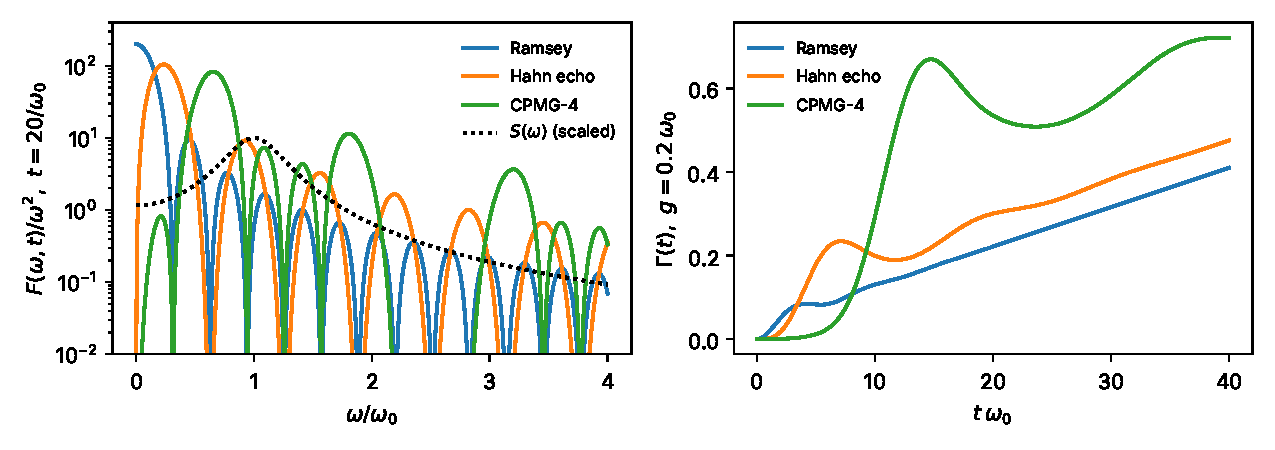
\includegraphics[width=\textwidth]{figures/fig_filter.pdf}
\caption{Left: filter functions $F(\omega,t)/\omega^2$ at $t=20/\omega_0$ for free induction, Hahn echo and CPMG with four pulses, against the Lorentzian noise spectrum of the running example.
Right: the resulting $\Gamma(t)$ (computed for the coupling $\tfrac12\sz\otimes B$, i.e.\ with $1/\pi$ in \cref{eq:filter}) at $g=0.2\omega_0$.
The CPMG curve shows a bump near $t\omega_0\approx4\pi$, where the comb's first tooth $\pi/\tau=4\pi/t$ sweeps through the bath resonance at $\Omega=\omega_0$: the sequence has detected the spectral line.}
\label{fig:filter}
\end{figure}

\subsection{The mixed sensor}

For general $\theta$ both channels are open.
In the secular (weak-coupling, long-time) regime the Ramsey signal decays at $\Gamma_2=\tfrac12\Gamma_1+\Gamma_\varphi$ with $\Gamma_1\propto\sin^2\theta\,S(\omega_0)$ and $\Gamma_\varphi\propto\cos^2\theta\,S(0)$, so a Ramsey measurement alone cannot separate low-frequency from resonant noise; a $T_1$ measurement is needed to subtract the $\Gamma_1/2$ part.
Dynamical decoupling filters only the $\cos^2\theta$ part: $\pi$-pulses about $\hat x$ commute with $\sx$, so the transverse coupling is not refocused, and the echo decay saturates at $\ee^{-\Gamma_1t/2}$.
Outside the secular regime the cross terms $\cos\theta\sin\theta$ of \cref{eq:K2-bloch} mix populations and coherences, and the pseudomode numerics of \cref{fig:dynamics} is the honest way to design a protocol.

\subsection{Precision scaling: when memory matters}

Frequency estimation by Ramsey interferometry with $N$ qubits and total time $T$: each run of duration $t$ yields a signal $\tfrac12[1+\ee^{-\Gamma(t)}\cos\omega_0t]$, with Fisher information $t^2\ee^{-2\Gamma(t)}$ per qubit per run at the optimal phase~\cite{Braunstein1994}.
With $T/t$ runs the Cram\'er--Rao bound reads
\begin{equation}
  \delta\omega_0^2\ \ge\ \frac{1}{N\,T\,t\,\ee^{-2\Gamma(t)}}\qquad\text{(product state)},\qquad
  \delta\omega_0^2\ \ge\ \frac{1}{N^2\,T\,t\,\ee^{-2N\Gamma(t)}}\qquad\text{(GHZ state)},
\end{equation}
the Greenberger--Horne--Zeilinger (GHZ) state~\cite{GHZ1989} acquiring the phase $N\omega_0t$ but, for independent baths, also $N$ times the dephasing exponent.
Optimizing over $t$:
\begin{center}
\renewcommand{\arraystretch}{1.3}
\begin{tabular}{@{}lll@{}}
\toprule
& product state & GHZ state\\
\midrule
Markov, $\Gamma=\gamma t$ & $t^*=\tfrac1{2\gamma}$, $\ \delta\omega_0^2=\dfrac{2e\gamma}{NT}$ & $t^*=\tfrac{1}{2N\gamma}$, $\ \delta\omega_0^2=\dfrac{2e\gamma}{NT}$ (no gain)\\[6pt]
Zeno regime, $\Gamma=\kappa t^2$ & $t^*=\tfrac{1}{2\sqrt\kappa}$, $\ \delta\omega_0^2=\dfrac{2\sqrt{e\kappa}}{NT}$ & $t^*=\tfrac{1}{2\sqrt{N\kappa}}$, $\ \delta\omega_0^2=\dfrac{2\sqrt{e\kappa}}{N^{3/2}T}$\\
\bottomrule
\end{tabular}
\end{center}
The first row is the classic result that Markovian dephasing erases the quantum advantage of entanglement~\cite{Huelga1997}.
The second row is the observation of Matsuzaki, Benjamin and Fitzsimons~\cite{Matsuzaki2011} and of Chin, Huelga and Plenio~\cite{Chin2012}: when the optimal interrogation time falls inside the initial quadratic (Zeno) regime of $\Gamma(t)$, which it does for a GHZ state at large $N$ because $t^*\propto N^{-1/2}$, the precision scales as $N^{-3/4}$, between the standard quantum limit $N^{-1/2}$ and the Heisenberg limit $N^{-1}$.
In the language of these notes: the short-time behaviour $\Gamma(t)\simeq2g^2t^2\cdot(\ldots)$ follows from $K(0)=K^{(2)}(0)\ne0$ (\cref{sec:nz-irreducible}): a memory kernel that is finite at $\tau=0$ always produces a quadratic onset, and the crossover time to linear decay is the bath correlation time $\tau_B$.
The Markov row applies when $t^*\gg\tau_B$, the Zeno row when $t^*\ll\tau_B$.
The numbers in \cref{eq:lorentz-kernels} give $\kappa=2g^2\cos^2\theta+g^2\sin^2\theta$ (dephasing plus half of the transverse channel) and $\tau_B=2/\gamma$ for the Lorentzian bath.

\subsection{Which formalism for which question}

\begin{center}
\small
\renewcommand{\arraystretch}{1.25}
\begin{tabularx}{\textwidth}{>{\raggedright\arraybackslash}p{4.2cm}>{\raggedright\arraybackslash}X}
\toprule
\textbf{Question} & \textbf{Natural tool}\\
\midrule
Which bath quantity does protocol X measure? & Keldysh rotation: $\qu\qu$ lines $\to S$, $\qu\cl$ lines $\to\chi$; read off from the diagram (\cref{sec:lec4}).\\
Exact dephasing under arbitrary control & Influence functional with c-number $y(s)$ (\cref{sec:lec7}); filter functions.\\
Rates, steady state, thermometry & Second-order NZ/TCL, secular limit (\cref{sec:lec5}); FDT fixes $\chi''/S$.\\
Short-time (Zeno) behaviour, precision scaling & TCL2 running rates (\cref{sec:lec6}); $K(0)\neq0$.\\
Strong coupling, incoherent regime & Polaron frame, NIBA and beyond (\cref{sec:lec7}).\\
Linear response of the sensor to a drive & Mori / retarded self-energy (\cref{sec:lec8}).\\
Back-action on the bath (a cavity, a line) & Keldysh Dyson equation for the dressed bath propagator (\cref{sec:lec9}).\\
Benchmarking any of the above & Pseudomode exact solution (\cref{sec:lec2,sec:numerics}).\\
\bottomrule
\end{tabularx}
\end{center}

\subsection{Exercises}

\begin{exercise}\label{ex:10-1}
Derive \cref{eq:kofman} from the running rate $\Gamma_\downarrow(t)=2\sin^2\theta\,\Re\int_0^t\ee^{i\omega_0\tau}C(\tau)\dd\tau$ and show that a periodic modulation of $\omega_0$ shifts the filter.
Explain the anti-Zeno effect for a bath whose $C(\omega)$ rises above $\omega_0$.
\end{exercise}

\begin{exercise}\label{ex:10-2}
Derive the Hahn-echo filter $F=8\sin^4(\omega t/4)$ and \cref{eq:comb}.
Use the Lorentzian $S(\omega)$ to reproduce the bump in \cref{fig:filter} analytically: at what $t$ does it appear for CPMG with $n$ pulses?
\end{exercise}

\begin{exercise}\label{ex:10-3}
Repeat the Fisher-information analysis for $T_1$-limited sensing (a transverse sensor) and for a Ramsey sensor with $\Gamma(t)=\Gamma_2t+\kappa t^2$.
Where is the crossover between the two rows of the table, in terms of $\tau_B$ and $N$?
\end{exercise}

\begin{exercise}\label{ex:10-4}
(Capstone.)
For the Lorentzian bath with $\theta=\pi/4$, use the pseudomode script to simulate a Hahn echo (insert a $\pi$-pulse about $\hat x$ at $t/2$) and compare the echo amplitude with (a) the filter-function prediction using only the $\cos^2\theta$ part and (b) the same multiplied by $\ee^{-\Gamma_1t/2}$.
Discuss the residual discrepancy in terms of the $\cos\theta\sin\theta$ terms of \cref{eq:K2-bloch}.
\end{exercise}

\clearpage

%=====================================================================
\appendix
\section{The numerical companion}
\label{sec:numerics}

All figures are produced by \texttt{figures/spin\_boson\_numerics.py} (NumPy, SciPy, Matplotlib; about one minute on a laptop).
This appendix records what it computes, so that each curve can be traced to an equation in the text.

\paragraph{Model and parameters.}
$\omega_0=1$ (units), $S=\cos\theta\sz+\sin\theta\sx$ with $\theta=\pi/4$, Lorentzian bath with $\Omega=1$, $\gamma=0.5$, $T=0$, couplings $g=0.1$ and $0.3$; initial state $\ket{+x}$; time step $\dd t=0.02$, $t\le40$.
Kernels: \cref{eq:lorentz-kernels}.

\paragraph{Representation.}
Column-stacking vectorization, \cref{eq:vec}: $A^+=\Id\otimes A$, $A^-=A^T\otimes\Id$, $A^\cl=\tfrac12(A^++A^-)$, $A^\qu=A^+-A^-$, $\Lc=-iH^\qu$.
Bloch-basis matrix elements are $M_{\mu\nu}=\tfrac12\Tr(\sigma_\mu\mathcal M\sigma_\nu)$ (the coefficient convention of \cref{sec:lec1}).

\paragraph{Exact reference.}
The pseudomode master equation \eqref{eq:pseudomode} with $N=14$ oscillator levels (checked against $N=20$: maximal deviation $5\times10^{-15}$ in $\Pi(t)$ for $t\le4$ at $g=0.3$).
$\Pi(t)$ is obtained by propagating the four basis operators $\ket i\bra j\otimes\ket0\bra0$ with $\ee^{\Lc_{\rm tot}\dd t}$ and tracing out the oscillator.
The exact TCL generator is $\Gc(t)=\dot\Pi\Pi^{-1}-\Lc_S$ with $\dot\Pi$ computed from $\Lc_{\rm tot}$ (no numerical differentiation).
The exact NZ kernel is computed directly from its definition \eqref{eq:NZ}, $K(\tau)=\Pc\Lc_I\ee^{\Qc\Lc\tau}\Qc\Lc_I\Pc$, with $\Pc=\Tr_{\rm osc}(\cdot)\otimes\ket0\bra0$ built as a matrix on the $(2N)^2$-dimensional Liouville space of qubit plus oscillator; since the kernel is determined by $\Pi(t)$ alone (Exercise~\ref{ex:5-4}), it is also the kernel of the physical Lorentzian bath.

\paragraph{Approximations.}
$K^{(2)}(\tau)$ from \cref{eq:K2}; NZ2 solves the Volterra equation with the trapezoidal rule and an implicit treatment of $K(0)\rho_n$; TCL2 uses $\Gc^{(2)}(t)=\int_0^tK^{(2)}(\tau)\ee^{-\Lc_S\tau}\dd\tau$ (cumulative trapezoid) and the midpoint exponential; Markov uses $\Gc^{(2)}(t_{\max})$.

\paragraph{Checks printed by the script} (for $g=0.3$):
\begin{center}
\small
\begin{tabular}{@{}lll@{}}
\toprule
quantity & analytic (\cref{sec:lec5}) & numerical ($\Gc^{(2)}_\infty$)\\
\midrule
$\Gamma_\downarrow$, $\Gamma_\uparrow$ & $0.36000$, $0.00554$ & --- \\
$1/T_1=-\Gc_{zz}$ & $0.36554$ & $0.36552$\\
$1/T_2=-\tfrac12(\Gc_{xx}+\Gc_{yy})$ & $0.22512$ & $0.22512$\\
$\Gamma_\varphi=-\Gc_{xx}$ & $0.04235$ & $0.0424$\\
$\tilde\omega_0$ (secular / nonsecular) & $1.0222$ & $1.0219$\\
$r_z^{\rm eq}=\Gc_{z\Id}/(-\Gc_{zz})$ & $-0.96970$ & $-0.96970$\\
\bottomrule
\end{tabular}
\end{center}
The small differences are the $\dd t$ discretization and the nonsecular versus secular definitions.
The nonsecular generator has $\Gc_{xx}=-\Gamma_\varphi$ and $\Gc_{yy}=-\Gamma_\varphi-\Gamma_1$, whose average is $\Gamma_2$ (Example~5.3), and $\Gc_{yx}=2\delta\omega$, $\Gc_{xy}=0$.

\paragraph{Check of Theorem~\ref{thm:irreducible}.}
The function \texttt{check\_fourth\_order} evaluates the fourth-order irreducible kernel $K^{(4)}$ as a double time integral of $\Pc\Lc_I\ee^{\Lc_0\cdot}\Qc\Lc_I\ee^{\Lc_0\cdot}\Qc\Lc_I\ee^{\Lc_0\cdot}\Qc\Lc_I\Pc$ in the pseudomode space and compares $K-K^{(2)}$ with $K^{(4)}$ for $g=0.05,0.1,0.2$ (Example~5.1).

\paragraph{Check of Example~5.4.}
The function \texttt{check\_rwa\_kernel} builds the rotating-wave pseudomode model, $H_I=g(\sigma_+a+\sigma_-a^\dagger)$ with the same $\Omega=\omega_0$ and $\gamma$ (truncation $N=4$ suffices at $T=0$, where at most one excitation is ever present), evaluates $\Pc\Lc_I\ee^{\Qc\Lc\tau}\Qc\Lc_I\Pc$ literally, and compares the $ee$ and $eg$ elements with the closed forms \eqref{eq:Kee-exact-t} and \eqref{eq:Keg-exact} at $\tau\omega_0=0,0.5,1,2,4,8$ for $g=0.1,0.3$ (agreement $3\times10^{-17}$), then compares $K_{ee}-K^{(2)}_{ee}$ with the fourth-order term of \cref{eq:Kee-geometric} for $g=0.05,0.1,0.2$.

\paragraph{Check of \cref{sec:ill}.}
The function \texttt{check\_influence\_kernel} builds the discretized Feynman--Vernon path sum \eqref{eq:ill-U} in the $S$ eigenbasis for the Lorentzian bath ($\eta_n$ from \cref{eq:ill-eta}, $4^N$ paths) and prints: (i) $|U_N-\Pi(N\Delta t)|$ for $\Delta t=0.2,0.1,0.05$; (ii) the transfer tensors \eqref{eq:ill-ttm} computed from the exact $\Pi$ against the continuous kernel $K(n\Delta t)$; (iii) the transfer tensors of the Trotterized $U_N$ against the chain formula \eqref{eq:ill-chain} for $n\le3$; (iv) the inverse map \eqref{eq:ill-inverse}; (v) the Hamiltonian-learning numbers of Example~7.3, with Trotter-consistent and with exact input.
It runs in a few seconds.

\paragraph{Filter functions.}
\Cref{fig:filter} evaluates \cref{eq:filter} with the $1/\pi$ normalization (coupling $\tfrac12\sz\otimes B$) and $g=0.2$, for Ramsey, Hahn and CPMG-4 sequences.

\clearpage

%=====================================================================
\section{Solutions and hints}
\label{sec:solutions}

\paragraph{Exercise~\ref{ex:1-1}.}
$(A^\cl)^\dagger$: $(X,A^\cl Y)=\tfrac12\Tr[X^\dagger(AY+YA)]=\tfrac12\Tr[(AX+XA)^\dagger Y]=(A^\cl X,Y)$ using
$A=A^\dagger$ and cyclicity. $(A^\qu)^\dagger$: $(X,[A,Y])=\Tr[X^\dagger AY-X^\dagger YA]=\Tr[(AX-XA)^\dagger(-1)\cdots]$,
giving $-(A^\qu X,Y)$. Hence $iA^\qu$ is Hermitian and $\Lc=-iH^\qu$ is anti-Hermitian, as the
generator of a unitary (isometric) evolution in Liouville space must be.

\paragraph{Exercise~\ref{ex:1-2}.}
With $\mathrm{vec}$ in the basis $\{\ket0\bra0,\ket0\bra1,\ket1\bra0,\ket1\bra1\}$,
$\Lc_S=-i(\Id\otimes H_S-H_S^T\otimes\Id)=\operatorname{diag}(0,-i\omega_0,i\omega_0,0)$. The change of basis to
$\sigma_\mu/\sqrt2$ is the unitary with columns $\mathrm{vec}(\sigma_\mu)/\sqrt2$; it maps the
$2\times2$ block $\operatorname{diag}(-i\omega_0,i\omega_0)$ on $(\ket0\bra1,\ket1\bra0)$ to the real rotation generator
$\begin{psmallmatrix}0&-\omega_0\\ \omega_0&0\end{psmallmatrix}$ on $(\sx,\sy)$.

\paragraph{Exercise~\ref{ex:1-3}.}
Trace preservation fixes the first row; Hermiticity preservation makes the matrix
real. For a unital qubit map with $T=\operatorname{diag}(\lambda_1,\lambda_2,\lambda_3)$, positivity is
$|\lambda_i|\le1$ while complete positivity (Fujiwara--Algoet conditions) is
$|\lambda_1\pm\lambda_2|\le|1\pm\lambda_3|$; transposition $(1,-1,1)$ violates the latter.

\paragraph{Exercise~\ref{ex:1-4}.}
$(S^\cl)^2=\tfrac14(S^{+}+S^{-})^2=\tfrac14(2+2S^+S^-)$ using $S^2=\Id$: it maps $X\mapsto\tfrac12(X+SXS)$. Similarly
$(S^\qu)^2X=2X-2SXS$. Hence $(S^\cl)^2+\tfrac14(S^\qu)^2=1$ and $(S^\cl)^2-\tfrac14(S^\qu)^2=S^+S^-$, i.e.\
$X\mapsto SXS$. In matrix form, $(S^\cl)^2$ projects onto $\mathrm{span}(\Id,S)$ and $\tfrac14(S^\qu)^2$
onto its complement (the two Pauli directions orthogonal to $\hat n$).

\paragraph{Exercise~\ref{ex:1-5}.}
$[A^+,B^+]X=ABX-BAX=([A,B])^+X$; $[A^-,B^-]X=XBA-XAB=-([A,B])^-X$; $[A^+,B^-]X=AXB-AXB=0$.
For \cref{eq:product-clqu} insert $A^\pm=A^\cl\pm\tfrac12A^\qu$ into $(AB)^\cl=\tfrac12(A^+B^++B^-A^-)$:
$A^+B^+=A^\cl B^\cl+\tfrac12A^\cl B^\qu+\tfrac12A^\qu B^\cl+\tfrac14A^\qu B^\qu$ and
$B^-A^-=B^\cl A^\cl-\tfrac12B^\cl A^\qu-\tfrac12B^\qu A^\cl+\tfrac14B^\qu A^\qu$; adding and halving gives the
anticommutators and the two commutators, and subtracting gives $(AB)^\qu$. For
$A=\sx$, $B=\sy$ the commutator terms are essential: the two anticommutator terms cancel
each other, $\tfrac12\{\sx^\cl,\sy^\cl\}=-\tfrac18\{\sx^\qu,\sy^\qu\}$: the first swaps $\sx\leftrightarrow\sy$ with
weight $\tfrac12$ and annihilates $\Id$ and $\sz$, the second is its negative (check with the
matrices of Example~1.2), while $\tfrac14([\sx^\cl,\sy^\qu]+[\sx^\qu,\sy^\cl])=i\sz^\cl$ exactly, which is the
whole answer $(\sx\sy)^\cl=(i\sz)^\cl$. The script
\texttt{spin\_boson\_numerics.py} contains the vectorized superoperators; the identities
hold to machine precision for random $A,B$.

\paragraph{Exercise~\ref{ex:2-1}.}
Straightforward from $b_k(t)=b_k\ee^{-i\omega_kt}$, $\avg{b_k^\dagger b_k}=\bar n_k$, $\avg{b_kb_k^\dagger}=\bar n_k+1$.

\paragraph{Exercise~\ref{ex:2-2}.}
From \cref{eq:chi-def}, $\chi(\omega)=\tfrac2\pi\int_0^\infty\dd\omega'J(\omega')\,I(\omega,\omega')$ with
$I(\omega,\omega')=\int_0^\infty\dd t\,\ee^{i\omega t}\sin\omega't$. This integral does not converge in the
ordinary sense; it is defined as a distribution by a convergence factor $\ee^{-\epsilon t}$,
$\epsilon\to0^+$ (adiabatic switching; the one-sided range comes from the $\theta(t)$ in
$\chi$). \emph{Step 1.} For real $k$,
\begin{equation*}
  \int_0^\infty\!\dd t\,\ee^{ikt-\epsilon t}=\frac{1}{\epsilon-ik}=\frac{\epsilon}{k^2+\epsilon^2}+i\,\frac{k}{k^2+\epsilon^2}
  \ \xrightarrow{\epsilon\to0^+}\ \pi\delta(k)+i\,\mathrm P\frac1k ,
\end{equation*}
because the Lorentzian $\epsilon/(k^2+\epsilon^2)$ has width $\epsilon$ and area $\pi$, while
$k/(k^2+\epsilon^2)$ is odd and equals $1/k$ away from $k=0$ (Sokhotski--Plemelj). Compare the
two-sided integral $\int_{-\infty}^\infty\ee^{ikt}\dd t=2\pi\delta(k)$: the one-sided one is half the
delta plus the odd principal-value part that the other half would cancel.
\emph{Step 2.} Write $\sin\omega't=(\ee^{i\omega't}-\ee^{-i\omega't})/2i$ and apply Step 1 with
$k=\omega\pm\omega'$:
\begin{align*}
  I&=\frac{1}{2i}\Big[\pi\delta(\omega+\omega')-\pi\delta(\omega-\omega')+i\,\mathrm P\frac{1}{\omega+\omega'}-i\,\mathrm P\frac{1}{\omega-\omega'}\Big],\\
  \Re I&=\frac12\Big[\mathrm P\frac{1}{\omega+\omega'}-\mathrm P\frac{1}{\omega-\omega'}\Big]=-\,\mathrm P\frac{\omega'}{\omega^2-\omega'^2},\qquad
  \Im I=\frac\pi2\big[\delta(\omega-\omega')-\delta(\omega+\omega')\big].
\end{align*}
(Without complex exponentials: $\int_0^\infty\sin\omega't\,\sin\omega t\,\ee^{-\epsilon t}\dd t
=\tfrac12\big[\tfrac{\epsilon}{(\omega-\omega')^2+\epsilon^2}-\tfrac{\epsilon}{(\omega+\omega')^2+\epsilon^2}\big]$, two Lorentzians
that become the two deltas.) \emph{Step 3.} Insert into $\chi(\omega)$. The deltas are
integrated against $J(\omega')$ over $\omega'>0$, so for $\omega>0$ only $\delta(\omega-\omega')$ fires and
$\chi''(\omega)=J(\omega)$, while for $\omega<0$ only $\delta(\omega+\omega')$ fires, with its minus sign, and
$\chi''(\omega)=-J(-\omega)$: together $\chi''(\omega)=\sgn(\omega)J(|\omega|)$, odd in $\omega$ as a dissipative
response must be. The real part of the same formula gives
$\chi'(\omega)=\tfrac2\pi\,\mathrm P\!\int_0^\infty\dd\omega'\,\omega'J(\omega')/(\omega'^2-\omega^2)$, the Kramers--Kronig relation
of \cref{sec:lec2}: one regularized integral yields both the dissipative part (deltas) and
the reactive part (principal value), tied together by the causal $\theta(t)$. Two
remarks. The sign of $i\epsilon$ is the only place where retarded versus advanced is
decided: $\int_{-\infty}^0\ee^{ikt+\epsilon t}\dd t=\pi\delta(k)-i\mathrm P(1/k)$, same deltas, opposite
principal value, hence $\chi^A(\omega)=\chi^R(\omega)^*$. And the finite-time version,
$\Re\int_0^t\ee^{i(\omega-\omega_0)\tau}\dd\tau=\sin[(\omega-\omega_0)t]/(\omega-\omega_0)\to\pi\delta(\omega-\omega_0)$, is the filter of
\cref{eq:kofman} that turns the running rates of \cref{sec:lec6} into Markov rates: a sharp
cutoff in time instead of an exponential one.

For the finite-$T$ Ohmic
kernel use $\int_0^\infty\omega\coth(\beta\omega/2)\cos\omega t\,\dd\omega=-(\pi/\beta)^2/\sinh^2(\pi t/\beta)$ for $t\ne0$ (the
$t=0$ singularity carries the positive weight that makes $S(\omega)\ge0$). $S(t)<0$ for all
$t>0$ is compatible with $S(\omega)\ge0$ because $S(\omega)=\int S(t)\ee^{i\omega t}\dd t$ is dominated by the
short-time peak.

\paragraph{Exercise~\ref{ex:2-3}.}
The adjoint master equation gives $\dot a=-(i\Omega+\gamma/2)a$ for the Heisenberg operator
in the absence of the qubit; with the quantum regression theorem,
$\avg{a(t)a^\dagger}=\ee^{-(i\Omega+\gamma/2)t}$. Gaussianity: the Lindbladian is quadratic in
$a,a^\dagger$, so it maps Gaussian states to Gaussian states.

\paragraph{Exercise~\ref{ex:2-4}.}
$\Tr_B[(\cos\theta\sz+\sin\theta\sx)B\cdots(\cos\theta\sz+\sin\theta\sx)B]$ contains $\cos\theta\sin\theta\,C(t)$ cross
terms between $\sz$ and $\sx$ vertices. Two independent baths would give
$C_{zz}=\cos^2\theta C$, $C_{xx}=\sin^2\theta C$, $C_{zx}=0$. The cross terms are the $cs$ entries of
\cref{eq:K2-bloch}.

\paragraph{Exercise~\ref{ex:3-1}.}
Eight terms $\tilde\Lc_I^{a_1}\tilde\Lc_I^{a_2}\tilde\Lc_I^{a_3}$, $a_i=\pm$, each a contour-ordered
three-point function of $B$, which vanishes for a Gaussian state with $\avg B=0$.

\paragraph{Exercise~\ref{ex:3-2}.}
For $t>s$: $D^{\cl\qu}=\tfrac12[C(t-s)-C(s-t)+C(t-s)-C(s-t)]=C(t-s)-C(s-t)=\avg{[B(t),B(s)]}$. For $t<s$ the
later superoperator is $B^\qu(s)$ and the trace identity kills the term. Without the table:
write $D^{ab}$ as $\Tr_B[\text{later}\cdot\text{earlier}\cdot\rhoB]$; if the later one is $B^\qu$ the
trace vanishes; if both are $B^\cl$ the result is symmetric in $t,s$.

\paragraph{Exercise~\ref{ex:3-3}.}
$\Tr_S[\tilde S^\cl(t)\tilde S^\cl(s)\rho_S]=\tfrac12\avg{\{\tilde S(t),\tilde S(s)\}}=\cos^2\theta+\sin^2\theta\cos\omega_0(t-s)$ for the
diagonal state (independent of $r_z$), and
$\Tr_S[\tilde S^\cl(t)\tilde S^\qu(s)\rho_S]=\avg{[\tilde S(t),\tilde S(s)]}=-2i\sin^2\theta\,r_z\sin\omega_0(t-s)$ for $t>s$: the
qubit's response function, proportional to its polarization, as a two-level system's
susceptibility must be.

\paragraph{Exercise~\ref{ex:3-4}.}
See the text; $\chi''(\omega)=J(\omega)-J(-\omega)$ and $S(\omega)=J(\omega)+J(-\omega)$ give $S=\sgn(\omega)\chi''$ at $T=0$
only for $|\omega|$ where $J(-|\omega|)\ll J(|\omega|)$; the negative-frequency tail is the price of the
pseudomode.

\paragraph{Exercise~\ref{ex:4-1}.}
$\Tr_SK^{(2)}X=-\Tr_S[S^\qu(\cdots)]=0$ by the first trace identity for $S$. Hermiticity: with
$Y=\ee^{\Lc_S\tau}[S(\tau)S^\qu X-i\chi(\tau)S^\cl X]$, $Y^\dagger=\ee^{\Lc_S\tau}[-S(\tau)S^\qu X^\dagger+i\chi S^\cl X^\dagger]$, so
$(S^\qu Y)^\dagger=-S^\qu Y^\dagger=S^\qu\ee^{\Lc_S\tau}[S\,S^\qu-i\chi S^\cl]X^\dagger$ for Hermitian $X$.

\paragraph{Exercise~\ref{ex:4-2}.}
Input $\sz$: $S^\cl\sz=\cos\theta\,\Id$, $S^\qu\sz=-2i\sin\theta\,\sy$. Free rotation:
$\ee^{\Lc_S\tau}\sy=\cos\omega_0\tau\,\sy-\sin\omega_0\tau\,\sx$, $\ee^{\Lc_S\tau}\Id=\Id$. Then
$-S^\qu[\,S_\tau(-2i\sin\theta)(\cos\,\sy-\sin\,\sx)-i\chi_\tau\cos\theta\,\Id\,]$; use $S^\qu\Id=0$,
$S^\qu\sy=-2i\cos\theta\sx+2i\sin\theta\sz$, $S^\qu\sx=2i\cos\theta\sy$:
$=-S_\tau\sin\theta\,[-4\cos\theta\cos\,\sx+4\sin\theta\cos\,\sz-4\cos\theta\sin\,\sy]$, giving the last column of
\cref{eq:K2-bloch}. Input $\Id$: $S^\cl\Id=S$, $S^\qu\Id=0$; $\ee^{\Lc_S\tau}S=\cos\theta\sz+\sin\theta(\cos\,\sx+\sin\,\sy)$;
then $i\chi_\tau S^\qu[\cdots]=\chi_\tau[2cs(1-\cos)\sy+2cs\sin\,\sx-2s^2\sin\,\sz]$, the first column. The
$\sx,\sy$ columns are analogous. At $\theta=0$ only the $c^2$ block survives (dephasing of
$\sx,\sy$ at rate $4S_\tau$ with the rotation); at $\theta=\pi/2$ only the $s^2$ entries
(relaxation of $\sz$, dephasing of $\sy$ but not of $\sx$ in the lab frame, and the
$\chi$-driven inhomogeneity).

\paragraph{Exercise~\ref{ex:4-3}.}
The 15 pairings of six ordered points split into 10 irreducible and 5 reducible:
$(12)(34)(56)$, $(12)\times$\{2 irreducible 4-point\}, \{2 irreducible 4-point\}$\times(56)$.
(Irreducible chord diagrams: $1,1,2,10,74,\dots$)

\paragraph{Exercise~\ref{ex:4-4}.}
$\Gamma(t)=4\int_0^t\dd t_1\int_0^{t_1}\dd t_2\,g^2\ee^{-\gamma(t_1-t_2)/2}\cos\Omega(t_1-t_2)$. Short times:
$4g^2t^2/2=2g^2t^2$. Long times: $4t\int_0^\infty S(\tau)\dd\tau=2S(\omega{=}0)\,t$ with
$S(0)=2g^2(\gamma/2)/(\Omega^2+\gamma^2/4)$, the zero-frequency value of $J(\omega)+J(-\omega)$.

\paragraph{Exercise~\ref{ex:5-1}.}
$\Pc\Lc\Pc=\Lc_S\Pc$ uses $\Pc\Lc_I\Pc=0$; $\Pc\Lc\ee^{\Qc\Lc\tau}\Qc\Lc\Pc=\Pc\Lc_I\ee^{\Qc\Lc\tau}\Qc\Lc_I\Pc$ uses
$\Pc\Lc_0\Qc=0$. With $\avg B\ne0$, write $B=\avg B+\delta B$ and absorb $S\avg B$ into $H_S$.

\paragraph{Exercise~\ref{ex:5-2}.}
Secular reduction of \cref{eq:K2-bloch} with $\ee^{-\Lc_S\tau}$ acting on the input:
$\Gc_{xx}=-4c^2\int S$, $\Gc_{yy}=-4c^2\int S-4s^2\int S\cos\omega_0\tau$, $\Gc_{yx}=4s^2\int S\sin\omega_0\tau$,
$\Gc_{xy}=0$, $\Gc_{zz}=-4s^2\int S\cos\omega_0\tau$, $\Gc_{z\Id}=-2s^2\int\chi\sin\omega_0\tau$. Average $\Gc_{xx}$ and
$\Gc_{yy}$ (the difference oscillates at $2\omega_0$ in the rotating frame) to get $\Gamma_2$; the
precession frequency is $\sqrt{\omega_0(\omega_0+\Gc_{yx})}\simeq\omega_0+\tfrac12\Gc_{yx}$. The Lamb shift
contains $\int_0^\infty S\sin\omega_0\tau$ only: the $\chi$ terms sit in the first column, which is the
inhomogeneity, not a frequency. In the operator form, $\Delta(\omega)=\Im\int_0^\infty\ee^{i\omega s}C(s)\dd s=\int_0^\infty S\sin\omega s-\tfrac12\chi'(\omega)$
and $\delta\omega=\sin^2\theta[\Delta(\omega_0)-\Delta(-\omega_0)]$; $\chi'$ is even and cancels.

\paragraph{Exercise~\ref{ex:5-3}.}
Secular: $\Gc=-i[\tilde H_S,\cdot]+\Gamma_\downarrow\Dc[\sigma_-]+\Gamma_\uparrow\Dc[\sigma_+]+\tfrac12\Gamma_\varphi\Dc[\sz]$ with
$\Dc[L]X=LXL^\dagger-\tfrac12\{L^\dagger L,X\}$. Nonsecular Redfield for $\theta=\pi/2$ has
$\Gc_{xx}=0$, $\Gc_{yy}=-\Gamma_1$: starting from $\ket{+y}$ the Bloch vector initially shrinks along $y$
but not along $x$, which is fine; the violation appears through the $\Gc_{yx}=2\delta\omega$ term
combined with the inhomogeneity when $\delta\omega$ is comparable to $\Gamma_1$, i.e.\ when
$\gamma\gtrsim\omega_0$ so that $S(\omega)$ is broad.

\paragraph{Exercise~\ref{ex:5-4}.}
$K(0)=\Tr_B[\Lc_I\Qc\Lc_I(X\otimes\rhoB)]=\Tr_B[\Lc_I\Lc_I(X\otimes\rhoB)]$ since $\Pc\Lc_I\Pc=0$. Laplace:
invert \cref{eq:Dyson}. For $\theta=0$, $\hat\Pi_{01}(z)=\int_0^\infty\ee^{-(z+i\omega_0)t-\Gamma(t)}\dd t$, and
$\hat K_{01}(z)=z+i\omega_0-1/\hat\Pi_{01}$; expanding $\ee^{-\Gamma}=1-\Gamma+\Gamma^2/2-\dots$ with $\Gamma=O(g^2)$ produces
all powers of $g^2$ in $\hat K$: the irreducible crossed and nested diagrams do not cancel.

\paragraph{Exercise~\ref{ex:6-1}.}
$\Sigma(t)=\int_0^t\hat G(t,s)\Qc\tilde\Lc_I(s)\Pc\tilde G(s,t)\dd s$ is explicitly $O(\Lc_I)$ and vanishes at $t=0$.
Expanding $\hat G$, $\tilde G$ and $[1-\Sigma]^{-1}$ and using $\Pc\tilde\Lc_I\Pc=0$ gives
\cref{eq:TCL2} at second order and \cref{eq:TCL4} at fourth, where the subtracted terms
come from $\Pc\tilde\Lc_I\Sigma^2\Pc$ and from the expansion of $\tilde G(s,t)$ inside $\Sigma$. Odd
orders have an odd number of $B$'s.

\paragraph{Exercise~\ref{ex:6-2}.}
$\int_0^tS(\tau)\dd\tau=g^2\,\Re\big[(1-\ee^{-(\gamma/2-i\Omega)t})/(\gamma/2-i\Omega)\big]$; negative windows exist when
$\Omega>\gamma/2$, the first around $\Omega t\in(\pi,2\pi)$ for small $\gamma/\Omega$.

\paragraph{Exercise~\ref{ex:6-3}.}
With $\Pi^{(2)}(t)=\int_0^t\dd t_1\int_0^{t_1}\dd t_2\,\Pi_0(t-t_1)K^{(2)}(t_1-t_2)\Pi_0(t_2)$ and
$\Pi^{-1}=\Pi_0^{-1}-\Pi_0^{-1}\Pi^{(2)}\Pi_0^{-1}+\dots$, the fourth-order term of \cref{eq:TCLNZ} is
$\int K^{(4)}(t-s)\Pi_0(s)\Pi_0(t)^{-1}+\int K^{(2)}(t-s)[\Pi^{(2)}(s)\Pi_0(t)^{-1}-\Pi_0(s)\Pi_0(t)^{-1}\Pi^{(2)}(t)\Pi_0(t)^{-1}]$. The
bracket, written as a time-ordered integral, is $-\int\int\int$ of the products
$\avg{\Lc_I\Lc_I}\avg{\Lc_I\Lc_I}$ in the crossed and nested time orderings, which are exactly the
last two subtractions of \cref{eq:TCL4}; the reducible product is already absent from $K^{(4)}$.

\paragraph{Exercise~\ref{ex:6-4}.}
$\hat\rho_{ee}(z)=\widehat{|c_e|^2}(z)\rho_{ee}(0)$ and $\hat K_{ee}(z)=z-1/\widehat{|c_e|^2}(z)$; the Laplace
transform of $|c_e|^2$ is a rational function with poles at $-\gamma/2\pm i|d|/2$ and $-\gamma/2$,
so $\hat K$ is analytic to the right of them. The generator's rate $\gamma(t)$ has poles on the
real $t$ axis, so its Laplace transform does not exist as an ordinary function.

\paragraph{Exercise~\ref{ex:7-1}.}
Substitute $s^\pm=s^\cl\pm\tfrac12s^\qu$ and $C=S-\tfrac i2\chi$:
$(s^+_1-s^-_1)[Cs^+_2-C^*s^-_2]=s^\qu_1[S(s^+_2-s^-_2)-\tfrac i2\chi(s^+_2+s^-_2)]=s^\qu_1[Ss^\qu_2-i\chi s^\cl_2]$.
Induction: the sum over pairings of $2n$ commuting vertices is $\tfrac1{n!}(\text{one line})^n$.

\paragraph{Exercise~\ref{ex:7-2}.}
For a blip $s^\qu=\pm2$ on $[t_a,t_b]$, $-\int\!\!\int s^\qu Ss^\qu=-4\int_{t_a}^{t_b}\dd t_1\int_{t_a}^{t_1}\dd t_2\,S(t_1-t_2)=-Q_2(t_b-t_a)$
using $\ddot Q_2=4S$, $Q_2(0)=\dot Q_2(0)=0$. The blip--sojourn term with the preceding sojourn
$s^\cl=\pm1$ on $[t_0,t_a]$ gives $\pm i\cdot2\int_{t_a}^{t_b}\dd t_1\int_{t_0}^{t_a}\dd t_2\,\chi(t_1-t_2)$, which for
$t_0\to-\infty$ is $\mp iQ_1(t_b-t_a)$ with $\ddot Q_1=-2\chi$.

\paragraph{Exercise~\ref{ex:7-3}.}
$B_+(\tau)=\prod_kD(\alpha_k\ee^{i\omega_k\tau})$ with $\alpha_k=2g_k/\omega_k$. $D(\alpha_\tau)D(-\alpha)=\ee^{-i\alpha^2\sin\omega\tau}D(\alpha(\ee^{i\omega\tau}-1))$ and
$|\alpha(\ee^{i\omega\tau}-1)|^2=2\alpha^2(1-\cos\omega\tau)$, so $\avg{B_+(\tau)B_-(0)}=\ee^{-Q_2-iQ_1}$ and, with the
other ordering, $\avg{B_-(0)B_+(\tau)}=\ee^{-Q_2+iQ_1}$. Detailed balance: expand to first order
in $Q$, $\int_0^\infty\ee^{-i\varepsilon\tau}(-Q_2+iQ_1)\dd\tau$ picks $+2J(\varepsilon)[\coth(\beta\varepsilon/2)+1]/\varepsilon^2$, hence
$w_{\downarrow\leftarrow\uparrow}\propto1+n$, $w_{\uparrow\leftarrow\downarrow}\propto n$.

\paragraph{Exercise~\ref{ex:7-4}.}
(a) $\hat K^s(z)$ for the Ohmic kernel is
$\Delta^2\int_0^\infty\ee^{-z\tau}(1+\omega_c^2\tau^2)^{-\alpha}\cos(2\alpha\arctan\omega_c\tau)\,\dd\tau$; for $z\ll\omega_c$ it behaves as
$\hat K^s(z)\simeq\Delta^2\,\Gamma(1-2\alpha)\cos(\pi\alpha)\,z^{2\alpha-1}\omega_c^{-2\alpha}$, giving poles of $\hat P$ at
$z\sim\Delta_r\,\ee^{\pm i\pi/(2-2\alpha)}$ with $\Delta_r=\Delta(\Delta/\omega_c)^{\alpha/(1-\alpha)}\times O(1)$; for
$\alpha\ge\tfrac12$ the poles are on the negative real axis (incoherent
decay)~\cite[Sec.~V]{Leggett1987}. (b) See Example~7.2.

\paragraph{Exercise~\ref{ex:8-1}.}
Apply the identity to $i\mathsf LA$: $\dot A(t)=\ee^{i\mathsf Lt}i\mathsf LA=\ee^{i\mathsf Lt}[\mathsf P+\mathsf Q]i\mathsf LA$; the
$\mathsf P$ part is $i\Omega A(t)$, the $\mathsf Q$ part is expanded with the identity into $F(t)$ plus
$\int_0^t\ee^{i\mathsf L(t-s)}i\mathsf P\mathsf LF(s)\dd s$, and $i\mathsf P\mathsf LF(s)=A(A,A)^{-1}(A,i\mathsf LF(s))=-A(A,A)^{-1}(i\mathsf LA,F(s))=-AM(s)$
using self-adjointness of $\mathsf L$ and $(A,F)=0$.

\paragraph{Exercise~\ref{ex:8-2}.}
Project on the \emph{fluctuation} $A=\delta\sz=\sz-\avg{\sz}$, with
$(\delta\sz,\delta\sz)=1-\tanh^2(\beta\omega_0/2)$ (projecting on $\sz$ itself keeps the non-decaying
part $\avg{\sz}^2$ in $C(t)$ and gives a memory function that vanishes at $z=0$). Then
$i\mathsf L\delta\sz=i\sin\theta[\sx,\sz]B=2\sin\theta\,\sy B=F(0)$, $F(t)=2\sin\theta\,\sy(t)B(t)$ with
$\sy(t)=\sy\cos\omega_0t+\sx\sin\omega_0t$, and $\avg{\sy\sy(t)}=\cos\omega_0t+i\tanh(\beta\omega_0/2)\sin\omega_0t$,
$\avg{\sy(t)\sy}=$ its conjugate. Hence
\begin{equation*}
  (F,F(t))=2\sin^2\theta\big[\avg{\sy\sy(t)}C(-t)+\avg{\sy(t)\sy}C(t)\big]
  =4\sin^2\theta\Big[S(t)\cos\omega_0t-\tfrac12\tanh\tfrac{\beta\omega_0}{2}\,\chi(t)\sin\omega_0t\Big],
\end{equation*}
and $\hat M(0)=2\sin^2\theta[S(\omega_0)-\tanh(\beta\omega_0/2)\chi''(\omega_0)]/(1-\tanh^2)=2\sin^2\theta S(\omega_0)=\Gamma_1$
by the FDT. The response kernel enters with the system's polarization and is what makes the
normalization work out; there is no inhomogeneous term because the equilibrium value
sits in the reference state and the GLE describes the fluctuation around it.

\paragraph{Exercise~\ref{ex:8-3}.}
With $E_\mu=\sigma_\mu/\sqrt2$, $(E_\mu,\Lc^\dagger E_\nu)_B=\tfrac12\Tr[\sigma_\mu(i[H,\sigma_\nu])\rhoB]$, which is the transpose
of $\tfrac12\Tr[\sigma_\nu(-i[H,\sigma_\mu])\rhoB]$: Heisenberg generators are the transposes of
Schr\"odinger ones in a real orthonormal basis. The same holds for the kernel.

\paragraph{Exercise~\ref{ex:8-4}.}
In the RWA, $\mathsf Q i\mathsf L$ acting on $F\propto\sigma_-a^\dagger$-type operators closes on
$\sigma_-a$ (one excitation), and the second-level memory is the bath's own correlator
$\ee^{-(i\Omega+\gamma/2)t}$. The continued fraction $\hat C(z)=\tfrac12/[z+i\omega_0+g^2/(z+i\Omega+\gamma/2)]$ has the poles
of $c_e(t)$.

\paragraph{Exercise~\ref{ex:9-1}.}
Each $h^\cl$ derivative inserts an $S^\cl$ vertex as the \emph{last} operation before the trace
in at least one term; by the trace identity the full sum vanishes.

\paragraph{Exercise~\ref{ex:9-2}.}
$\sz=-i\eta_x\eta_y$, etc.; $\Theta\eta_x=-i\eta_x\eta_y\eta_z\eta_x=-i\eta_y\eta_z=\sx$. $H_I=S\otimes B$ becomes
$\Theta(\cos\theta\eta_z+\sin\theta\eta_x)B$; since $\Theta$ is conserved, in each sector $\Theta=\pm1$ the vertex is
linear in one Majorana and in $B$: the second-order self-energy of $\eta_i$ is a bath line
times a $\delta_{ij}$ Majorana loop-free diagram, i.e.\ $\Sigma_{\eta}\propto D$.

\paragraph{Exercise~\ref{ex:9-3}.}
Follow~\cite[Sec.~2]{Sieberer2016} with fermionic (Majorana) fields; the result is
$\Sigma^R=-i(\Gamma_\downarrow+\Gamma_\uparrow)/2$ and $\Sigma^K=-i(\Gamma_\downarrow-\Gamma_\uparrow)$ for the $\sigma_-$ propagator up to
normalization, so that $\Sigma^K/(\Sigma^R-\Sigma^A)=(\Gamma_\downarrow-\Gamma_\uparrow)/(\Gamma_\downarrow+\Gamma_\uparrow)=\tanh(\beta\omega_0/2)$ iff
detailed balance holds.

\paragraph{Exercise~\ref{ex:10-1}.}
Insert $C(\tau)=\int\frac{\dd\omega}{2\pi}C(\omega)\ee^{-i\omega\tau}$ and use $2\Re\int_0^t\ee^{i(\omega_0-\omega)\tau}\dd\tau=2\sin[(\omega-\omega_0)t]/(\omega-\omega_0)$.
A modulation $\omega_0\to\omega_0+\delta\cos\nu t$ replaces the sinc by a sum of sincs centred at $\omega_0+k\nu$
weighted by Bessel functions. If $C(\omega)$ grows above $\omega_0$ the broadened filter samples
more spectral weight and the decay accelerates (anti-Zeno).

\paragraph{Exercise~\ref{ex:10-2}.}
$\int_0^ty\ee^{i\omega s}\dd s=-\ee^{i\omega t/2}[2\cos(\omega t/2)-2]/(i\omega)$, so $|\cdot|^2=16\sin^4(\omega t/4)/\omega^2$. For the comb,
expand the square wave, $y=\tfrac4\pi\sum_{k\ \rm odd}k^{-1}\sin(k\pi s/\tau)$, and use
$|\int_0^t\ee^{i(\omega-k\pi/\tau)s}\dd s|^2\to2\pi t\,\delta(\omega-k\pi/\tau)$. The first tooth hits $\Omega$ when
$n\pi/t=\Omega$, i.e.\ $t=n\pi/\Omega$ ($=4\pi$ for $n=4$).

\paragraph{Exercise~\ref{ex:10-3}.}
Maximize $t\ee^{-2\Gamma_2t-2\kappa t^2}$: the quadratic term matters when $\kappa t^*\gtrsim\Gamma_2$, i.e.\
$t^*\lesssim\tau_B$; for GHZ states $t^*\sim1/(2N\Gamma_2)$, so the Zeno regime is reached for
$N\gtrsim1/(\Gamma_2\tau_B)$. For $T_1$-limited sensing (signal $\propto\ee^{-\Gamma_1t}$ with the phase on the
populations) the same algebra applies with $\Gamma_1$ in place of $2\Gamma_2$.

\paragraph{Exercise~\ref{ex:10-4}.}
Implement the pulse as $\rho\to\sx\rho\sx$ on the qubit factor at $t/2$ in the pseudomode
simulation. Expect (b) to be closer than (a), with a residual oscillating discrepancy of
relative size $\sim g^2\sin\theta\cos\theta/\omega_0$ at short times and a drift of the echo
``baseline'' from the $\chi$-driven inhomogeneity.


\bibliographystyle{unsrtnat}
\bibliography{refs}

\end{document}
